\documentclass[]{book}
\usepackage{lmodern}
\usepackage{amssymb,amsmath}
\usepackage{ifxetex,ifluatex}
\usepackage{fixltx2e} % provides \textsubscript
\ifnum 0\ifxetex 1\fi\ifluatex 1\fi=0 % if pdftex
  \usepackage[T1]{fontenc}
  \usepackage[utf8]{inputenc}
\else % if luatex or xelatex
  \ifxetex
    \usepackage{mathspec}
  \else
    \usepackage{fontspec}
  \fi
  \defaultfontfeatures{Ligatures=TeX,Scale=MatchLowercase}
\fi
% use upquote if available, for straight quotes in verbatim environments
\IfFileExists{upquote.sty}{\usepackage{upquote}}{}
% use microtype if available
\IfFileExists{microtype.sty}{%
\usepackage{microtype}
\UseMicrotypeSet[protrusion]{basicmath} % disable protrusion for tt fonts
}{}
\usepackage[margin=1in]{geometry}
\usepackage{hyperref}
\hypersetup{unicode=true,
            pdftitle={Introduction to Open Data Science},
            pdfauthor={Julie Lowndes \& The OHI Team},
            pdfborder={0 0 0},
            breaklinks=true}
\urlstyle{same}  % don't use monospace font for urls
\usepackage{color}
\usepackage{fancyvrb}
\newcommand{\VerbBar}{|}
\newcommand{\VERB}{\Verb[commandchars=\\\{\}]}
\DefineVerbatimEnvironment{Highlighting}{Verbatim}{commandchars=\\\{\}}
% Add ',fontsize=\small' for more characters per line
\usepackage{framed}
\definecolor{shadecolor}{RGB}{248,248,248}
\newenvironment{Shaded}{\begin{snugshade}}{\end{snugshade}}
\newcommand{\KeywordTok}[1]{\textcolor[rgb]{0.13,0.29,0.53}{\textbf{{#1}}}}
\newcommand{\DataTypeTok}[1]{\textcolor[rgb]{0.13,0.29,0.53}{{#1}}}
\newcommand{\DecValTok}[1]{\textcolor[rgb]{0.00,0.00,0.81}{{#1}}}
\newcommand{\BaseNTok}[1]{\textcolor[rgb]{0.00,0.00,0.81}{{#1}}}
\newcommand{\FloatTok}[1]{\textcolor[rgb]{0.00,0.00,0.81}{{#1}}}
\newcommand{\ConstantTok}[1]{\textcolor[rgb]{0.00,0.00,0.00}{{#1}}}
\newcommand{\CharTok}[1]{\textcolor[rgb]{0.31,0.60,0.02}{{#1}}}
\newcommand{\SpecialCharTok}[1]{\textcolor[rgb]{0.00,0.00,0.00}{{#1}}}
\newcommand{\StringTok}[1]{\textcolor[rgb]{0.31,0.60,0.02}{{#1}}}
\newcommand{\VerbatimStringTok}[1]{\textcolor[rgb]{0.31,0.60,0.02}{{#1}}}
\newcommand{\SpecialStringTok}[1]{\textcolor[rgb]{0.31,0.60,0.02}{{#1}}}
\newcommand{\ImportTok}[1]{{#1}}
\newcommand{\CommentTok}[1]{\textcolor[rgb]{0.56,0.35,0.01}{\textit{{#1}}}}
\newcommand{\DocumentationTok}[1]{\textcolor[rgb]{0.56,0.35,0.01}{\textbf{\textit{{#1}}}}}
\newcommand{\AnnotationTok}[1]{\textcolor[rgb]{0.56,0.35,0.01}{\textbf{\textit{{#1}}}}}
\newcommand{\CommentVarTok}[1]{\textcolor[rgb]{0.56,0.35,0.01}{\textbf{\textit{{#1}}}}}
\newcommand{\OtherTok}[1]{\textcolor[rgb]{0.56,0.35,0.01}{{#1}}}
\newcommand{\FunctionTok}[1]{\textcolor[rgb]{0.00,0.00,0.00}{{#1}}}
\newcommand{\VariableTok}[1]{\textcolor[rgb]{0.00,0.00,0.00}{{#1}}}
\newcommand{\ControlFlowTok}[1]{\textcolor[rgb]{0.13,0.29,0.53}{\textbf{{#1}}}}
\newcommand{\OperatorTok}[1]{\textcolor[rgb]{0.81,0.36,0.00}{\textbf{{#1}}}}
\newcommand{\BuiltInTok}[1]{{#1}}
\newcommand{\ExtensionTok}[1]{{#1}}
\newcommand{\PreprocessorTok}[1]{\textcolor[rgb]{0.56,0.35,0.01}{\textit{{#1}}}}
\newcommand{\AttributeTok}[1]{\textcolor[rgb]{0.77,0.63,0.00}{{#1}}}
\newcommand{\RegionMarkerTok}[1]{{#1}}
\newcommand{\InformationTok}[1]{\textcolor[rgb]{0.56,0.35,0.01}{\textbf{\textit{{#1}}}}}
\newcommand{\WarningTok}[1]{\textcolor[rgb]{0.56,0.35,0.01}{\textbf{\textit{{#1}}}}}
\newcommand{\AlertTok}[1]{\textcolor[rgb]{0.94,0.16,0.16}{{#1}}}
\newcommand{\ErrorTok}[1]{\textcolor[rgb]{0.64,0.00,0.00}{\textbf{{#1}}}}
\newcommand{\NormalTok}[1]{{#1}}
\usepackage{longtable,booktabs}
\usepackage{graphicx,grffile}
\makeatletter
\def\maxwidth{\ifdim\Gin@nat@width>\linewidth\linewidth\else\Gin@nat@width\fi}
\def\maxheight{\ifdim\Gin@nat@height>\textheight\textheight\else\Gin@nat@height\fi}
\makeatother
% Scale images if necessary, so that they will not overflow the page
% margins by default, and it is still possible to overwrite the defaults
% using explicit options in \includegraphics[width, height, ...]{}
\setkeys{Gin}{width=\maxwidth,height=\maxheight,keepaspectratio}
\IfFileExists{parskip.sty}{%
\usepackage{parskip}
}{% else
\setlength{\parindent}{0pt}
\setlength{\parskip}{6pt plus 2pt minus 1pt}
}
\setlength{\emergencystretch}{3em}  % prevent overfull lines
\providecommand{\tightlist}{%
  \setlength{\itemsep}{0pt}\setlength{\parskip}{0pt}}
\setcounter{secnumdepth}{5}
% Redefines (sub)paragraphs to behave more like sections
\ifx\paragraph\undefined\else
\let\oldparagraph\paragraph
\renewcommand{\paragraph}[1]{\oldparagraph{#1}\mbox{}}
\fi
\ifx\subparagraph\undefined\else
\let\oldsubparagraph\subparagraph
\renewcommand{\subparagraph}[1]{\oldsubparagraph{#1}\mbox{}}
\fi

%%% Use protect on footnotes to avoid problems with footnotes in titles
\let\rmarkdownfootnote\footnote%
\def\footnote{\protect\rmarkdownfootnote}

%%% Change title format to be more compact
\usepackage{titling}

% Create subtitle command for use in maketitle
\newcommand{\subtitle}[1]{
  \posttitle{
    \begin{center}\large#1\end{center}
    }
}

\setlength{\droptitle}{-2em}
  \title{Introduction to Open Data Science}
  \pretitle{\vspace{\droptitle}\centering\huge}
  \posttitle{\par}
  \author{Julie Lowndes \& The OHI Team}
  \preauthor{\centering\large\emph}
  \postauthor{\par}
  \predate{\centering\large\emph}
  \postdate{\par}
  \date{2017-11-21}

\usepackage{booktabs}
\usepackage{amsthm}
\makeatletter
\def\thm@space@setup{%
  \thm@preskip=8pt plus 2pt minus 4pt
  \thm@postskip=\thm@preskip
}
\makeatother

\usepackage{amsthm}
\newtheorem{theorem}{Theorem}[chapter]
\newtheorem{lemma}{Lemma}[chapter]
\theoremstyle{definition}
\newtheorem{definition}{Definition}[chapter]
\newtheorem{corollary}{Corollary}[chapter]
\newtheorem{proposition}{Proposition}[chapter]
\theoremstyle{definition}
\newtheorem{example}{Example}[chapter]
\theoremstyle{definition}
\newtheorem{exercise}{Exercise}[chapter]
\theoremstyle{remark}
\newtheorem*{remark}{Remark}
\newtheorem*{solution}{Solution}
\begin{document}
\maketitle

{
\setcounter{tocdepth}{1}
\tableofcontents
}
\chapter{Welcome}\label{welcome}

\textbf{Welcome.} \textbf{This training program is under active
development and testing}.

This 2-day training workshop will introduce you to open data science so
you can work with data in an open, reproducible, and collaborative way.
Open data science means that methods, data, and code are available so
that others can access, reuse, and build from it without much fuss. Here
you will learn a workflow with R, RStudio, Git, and GitHub, as we
describe in
\href{https://www.nature.com/articles/s41559-017-0160}{Lowndes \emph{et
al.} 2017: Our path to better science in less time using open data
science tools}.

This workshop is going to be fun, because learning these open data
science tools and practices is empowering! This training book is written
so you can use it as self-paced learning, or it can be used to teach an
in-person workshop. Either way, you should do everything hands-on on
your own computer as you learn.

Before you begin, be sure you are all set up: see Chapter
\ref{overview}: Overview and Prerequisites.

Suggested breakdown for a 2-day workshop:

\begin{longtable}[]{@{}lrr@{}}
\toprule
\begin{minipage}[b]{0.15\columnwidth}\raggedright\strut
time\strut
\end{minipage} & \begin{minipage}[b]{0.15\columnwidth}\raggedleft\strut
Day 1\strut
\end{minipage} & \begin{minipage}[b]{0.15\columnwidth}\raggedleft\strut
Day 2\strut
\end{minipage}\tabularnewline
\midrule
\endhead
\begin{minipage}[t]{0.15\columnwidth}\raggedright\strut
9-10:30\strut
\end{minipage} & \begin{minipage}[t]{0.15\columnwidth}\raggedleft\strut
Motivation, R and RStudio\strut
\end{minipage} & \begin{minipage}[t]{0.15\columnwidth}\raggedleft\strut
Wrangling (tidyr)\strut
\end{minipage}\tabularnewline
\begin{minipage}[t]{0.15\columnwidth}\raggedright\strut
break\strut
\end{minipage} & \begin{minipage}[t]{0.15\columnwidth}\raggedleft\strut
\strut
\end{minipage} & \begin{minipage}[t]{0.15\columnwidth}\raggedleft\strut
\strut
\end{minipage}\tabularnewline
\begin{minipage}[t]{0.15\columnwidth}\raggedright\strut
11-12:30\strut
\end{minipage} & \begin{minipage}[t]{0.15\columnwidth}\raggedleft\strut
GitHub, scripting in R\strut
\end{minipage} & \begin{minipage}[t]{0.15\columnwidth}\raggedleft\strut
Extended analysis (importing, for loops, etc)\strut
\end{minipage}\tabularnewline
\begin{minipage}[t]{0.15\columnwidth}\raggedright\strut
lunch\strut
\end{minipage} & \begin{minipage}[t]{0.15\columnwidth}\raggedleft\strut
\strut
\end{minipage} & \begin{minipage}[t]{0.15\columnwidth}\raggedleft\strut
\strut
\end{minipage}\tabularnewline
\begin{minipage}[t]{0.15\columnwidth}\raggedright\strut
13:30-15:00\strut
\end{minipage} & \begin{minipage}[t]{0.15\columnwidth}\raggedleft\strut
Visualization (gpplot2)\strut
\end{minipage} & \begin{minipage}[t]{0.15\columnwidth}\raggedleft\strut
Collaborating with GitHub\strut
\end{minipage}\tabularnewline
\begin{minipage}[t]{0.15\columnwidth}\raggedright\strut
break\strut
\end{minipage} & \begin{minipage}[t]{0.15\columnwidth}\raggedleft\strut
\strut
\end{minipage} & \begin{minipage}[t]{0.15\columnwidth}\raggedleft\strut
\strut
\end{minipage}\tabularnewline
\begin{minipage}[t]{0.15\columnwidth}\raggedright\strut
15:30-17:00\strut
\end{minipage} & \begin{minipage}[t]{0.15\columnwidth}\raggedleft\strut
Wrangling (dplyr)\strut
\end{minipage} & \begin{minipage}[t]{0.15\columnwidth}\raggedleft\strut
Extended analysis 2\strut
\end{minipage}\tabularnewline
\bottomrule
\end{longtable}

\textbf{License}

\chapter{Overview}\label{overview}

Welcome.

This is a 2-day training workshop to learn R, RStudio, Git, and GitHub,
and it's going to be fun and empowering. You will learn a reproducible
workflow that can be used in analyses of all kinds, including Ocean
Health Index assessments. This is really powerful, cool stuff, and not
just for data: I made and published this book using those four tools and
workflow.

We will practice learning three main things all at the same time: coding
with best practices (R/RStudio), collaborative version control
(Git/GitHub), and communication/publishing (RMarkdown/GitHub). This
training will teach these all together to reinforce skills and best
practices, and get you comfortable with a workflow that you can use in
your own projects.

\section{What to expect}\label{what-to-expect}

This is going to be a fun workshop.

The plan is to expose you to a lot of great tools that you can have
confidence using in your research. You'll be working hands-on and doing
the same things on your own computer as we do live on up on the screen.
We're going to go through a lot in these two days and it's less
important that you remember it all. More imporatantly, you'll have
experience with it and confidence that you can do it. The main thing to
take away is that there \emph{are} good ways to approach your analyses;
we will teach you to expect that so you can find what you need and use
it! And, you can use these materials as a reference as you go forward
with your analyses.

We'll be talking about :

\begin{itemize}
\tightlist
\item
  how to THINK about data. And not just any data; tidy data.
\item
  how to increase reproducibility in your science
\item
  how to more easily collaborate with others--including your future
  self!
\item
  how the \#rstats community is fantastic. The tools we're using are
  developed by real people. They are building great stuff and helping
  people of all skill-levels learn how to use it.
\end{itemize}

Everyone in this workshop is coming from a different place with
different experiences and expectations. But everyone will learn
something new here, because there is so much innovation in the data
science world. Even instructors and helpers learn something new every
time, from each other and from your questions.

You are all welcome here and encouraged to help each other.

\subsection{Tidy data workflow}\label{tidy-data-workflow}

We will be learning about tidy data.

\href{http://hadley.nz/}{\textbf{Hadley Wickham}} has developed a ton of
the tools we'll use today. Here's an overview of techniques to be
covered in Hadley Wickham and Garrett Grolemund of RStudio's book
\href{http://r4ds.had.co.nz/}{R for Data Science}:

\begin{figure}[htbp]
\centering
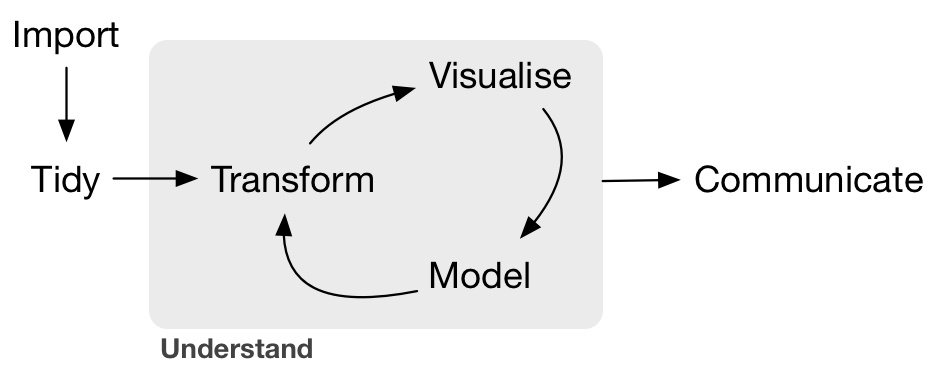
\includegraphics{img/r4ds_data-science.png}
\caption{}
\end{figure}

We will be focusing on:

\begin{itemize}
\tightlist
\item
  \textbf{Tidy}: \texttt{tidyr} to organize rows of data into unique
  values
\item
  \textbf{Transform}: \texttt{dplyr} to manipulate/wrangle data based on
  subsetting by rows or columns, sorting and joining
\item
  \textbf{Visualise}:

  \begin{itemize}
  \tightlist
  \item
    \texttt{ggplot2} static plots, using grammar of graphics principles
  \end{itemize}
\item
  \textbf{Communicate}

  \begin{itemize}
  \tightlist
  \item
    online website with \emph{Github Pages}
  \item
    version with \emph{git}
  \item
    dynamic documents with \emph{Rmarkdown}
  \end{itemize}
\end{itemize}

\section{Gapminder data:}\label{gapminder-data}

We'll be using the \href{http://www.gapminder.org/world}{gapminder
dataset} pioneered by
\href{https://www.ted.com/speakers/hans_rosling}{Hans Rosling}. These
data represent the health and wealth of every nation in the world.

While these data are not conservation or environmental oriented, it is a
fantastically rich data set with many parallels to data you may have and
wrangling you will need to do. It's important to be open to separate
your science questions from data questions, and working with other
people's data is a good way to do it. These data will be familiar to
data that you're likely working with: there is information for many
indicators for many study sites for many years.

\section{By the end of the
course\ldots{}}\label{by-the-end-of-the-course}

By the end of the course you'll wrangle the gapminder data, make your
own graphics that you'll publish on a webpage you've built with GitHub
and RMarkdown. Woop!

I made this training book with GitHub and RStudio's RMarkdown, which is
what we'll be learning in the workshop.

\section{Prerequisites}\label{prerequisites}

Before the training, please make sure you have done the following:

\begin{enumerate}
\def\labelenumi{\arabic{enumi}.}
\tightlist
\item
  Have up-to-date versions of \texttt{R} and RStudio and have RStudio
  configured with Git/GitHub

  \begin{itemize}
  \tightlist
  \item
    Download and install R: \url{https://cloud.r-project.org}
  \item
    Download and install RStudio: \url{http://www.rstudio.com/download}
  \item
    Create a GitHub account: \url{https://github.com} \emph{Note!
    Shorter names that kind of identify you are better, and use your
    work email!}
  \end{itemize}
\item
  Get comfortable: if you're not in a physical workshop, be set up with
  two screens if possible. You will be following along in RStudio on
  your own computer while also watching a virtual training or following
  this tutorial on your own.
\end{enumerate}

\section{Credit}\label{credit}

This material builds from a lot of fantastic materials developed by
others in the open data science community. In particular, it pulls from
the following resources, which are highly recommended for further
learning and as resources later on. Specific lessons will also cite more
resources.

\begin{itemize}
\tightlist
\item
  \href{http://r4ds.had.co.nz/}{R for Data Science} by Hadley Wickham
  and Garrett Grolemund
\item
  \href{http://stat545.com/}{STAT 545} by Jenny Bryan
\item
  \href{http://happygitwithr.com}{Happy Git with R} by Jenny Bryan
\item
  \href{https://software-carpentry.org/lessons/}{Software Carpentry} by
  the Carpentries
\end{itemize}

\chapter{R/RStudio Orientation, GitHub Setup}\label{orientation}

\section{Objectives \& Resources}\label{objectives-resources}

\textbf{Objectives}

In this lesson we will:

\begin{itemize}
\tightlist
\item
  get oriented to the RStudio interface
\item
  work with R in the console
\item
  be introduced to built-in R functions
\item
  learn to use the help pages
\item
  explore RMarkdown
\item
  configure git on our computers
\end{itemize}

\textbf{Resources}

This lesson is a combination of excellent lessons by others (thank you
Jenny Bryan and Data Carpentry!) that I have combined and modified for
our workshop today. I definitely recommend reading through the original
lessons and using them as reference:

\href{https://stat545-ubc.github.io/}{Dr.~Jenny Bryan's lectures from
STAT545 at UBC}

\begin{itemize}
\tightlist
\item
  \href{http://stat545-ubc.github.io/block002_hello-r-workspace-wd-project.html}{R
  basics, workspace and working directory, RStudio projects}
\item
  \href{http://stat545-ubc.github.io/block006_care-feeding-data.html}{Basic
  care and feeding of data in R}
\end{itemize}

RStudio has great resources about its IDE (IDE stands for integrated
development environment):

\begin{itemize}
\tightlist
\item
  \href{https://www.rstudio.com/resources/webinars/}{webinars}
\item
  \href{https://www.rstudio.com/resources/cheatsheets/}{cheatsheets}
\end{itemize}

\section{Why learn R with RStudio}\label{why-learn-r-with-rstudio}

You are all here today to learn how to code. Coding made me a better
scientist because I was able to think more clearly about analyses, and
become more efficient in doing so. Data scientists are creating tools
that make coding more intuitive for new coders like us, and there is a
wealth of awesome instruction and resources available to learn more and
get help.

Here is an analogy to start us off. \textbf{If you were a pilot, R is an
an airplane.} You can use R to go places! With practice you'll gain
skills and confidence; you can fly further distances and get through
tricky situations. You will become an awesome pilot and can fly your
plane anywhere.

And \textbf{if R were an airplane, RStudio is the airport}. RStudio
provides support! Runways, communication, community, and other services,
and just makes your overall life easier. So it's not just the
infrastructure (the user interface or IDE), although it is a great way
to learn and interact with your variables, files, and interact directly
with GitHub. It's also data science philosophy, R packages, community,
and more. So although you can fly your plane without an airport and we
could learn R without RStudio, that's not what we're going to do.

\begin{quote}
We are learning R together with RStudio and its many supporting
features.
\end{quote}

Something else to start us off is to mention that you are learning a new
language here. It's an ongoing process, it takes time, you'll make
mistakes, it can be frustrating, but it will be overwhelmingly awesome
in the long run. We all speak at least one language; it's a similar
process, really. And no matter how fluent you are, you'll always be
learning, you'll be trying things in new contexts, learning words that
mean the same as others, etc, just like everybody else. And just like
any form of communication, there will be miscommunications that can be
frustrating, but hands down we are all better off because of it.

While language is a familiar concept, programming languages are in a
different context from spoken languages, but you will get to know this
context with time. For example: you have a concept that there is a first
meal of the day, and there is a name for that: in English it's
``breakfast''. So if you're learning Spanish, you could expect there is
a word for this concept of a first meal. (And you'd be right:
`desayuno'). \textbf{We will get you to expect that programming
languages also have words (called functions in R) for concepts as well}.
You'll soon expect that there is a way to order values numerically. Or
alphabetically. Or search for patterns in text. Or calculate the median.
Or reorganize columns to rows. Or subset exactly what you want. We will
get you increase your expectations and learn to ask and find what you're
looking for.

\section{R at the console, RStudio
goodies}\label{r-at-the-console-rstudio-goodies}

Launch RStudio/R.

\begin{figure}[htbp]
\centering
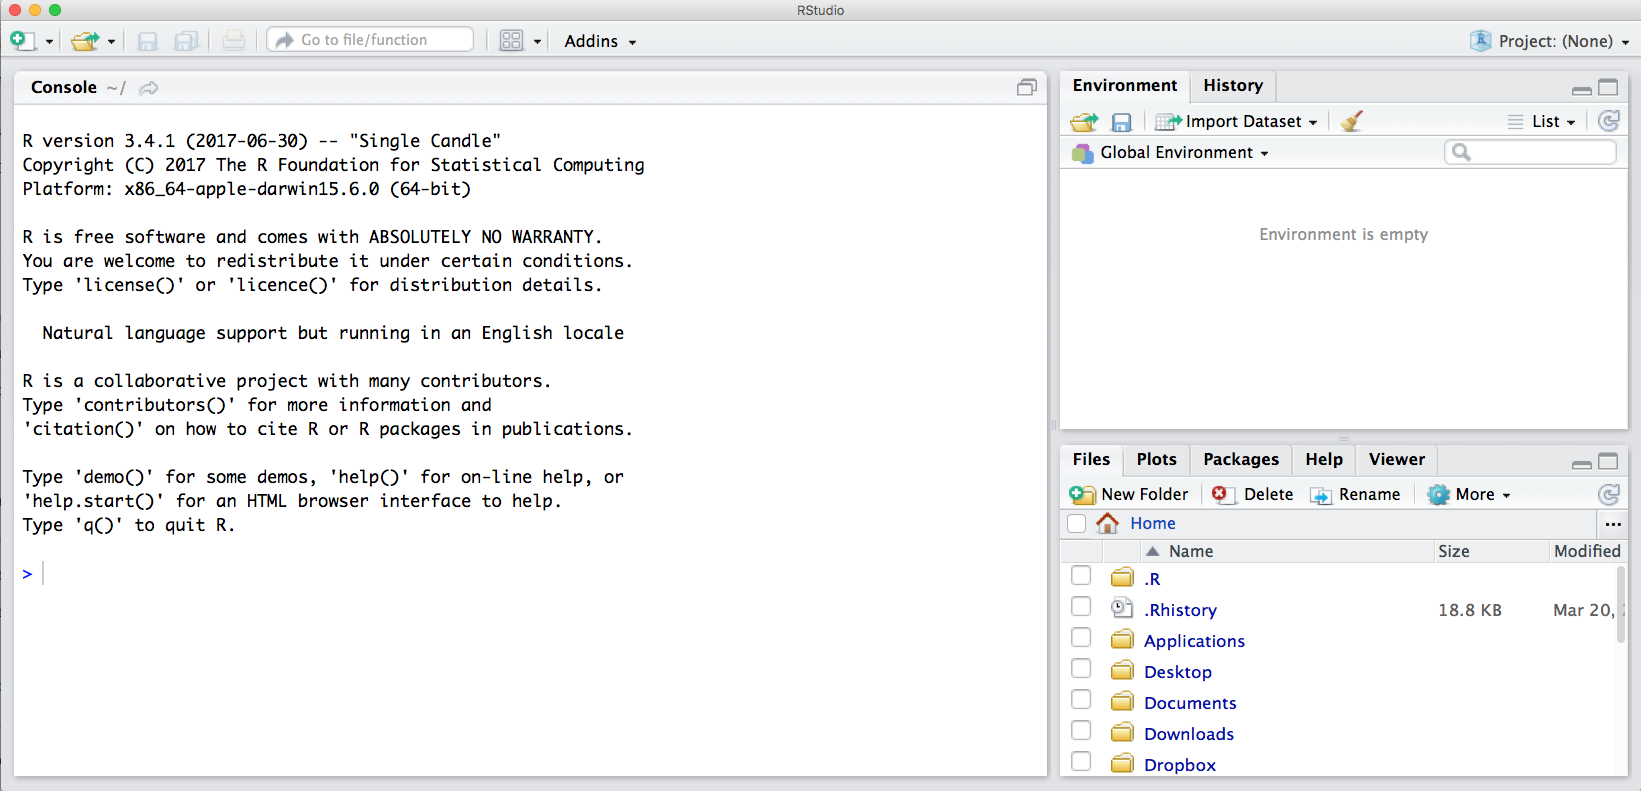
\includegraphics{img/RStudio_IDE.png}
\caption{}
\end{figure}

Notice the default panes:

\begin{itemize}
\tightlist
\item
  Console (entire left)
\item
  Environment/History (tabbed in upper right)
\item
  Files/Plots/Packages/Help (tabbed in lower right)
\end{itemize}

FYI: you can change the default location of the panes, among many other
things:
\href{https://support.rstudio.com/hc/en-us/articles/200549016-Customizing-RStudio}{Customizing
RStudio}.

An important first question: \textbf{where are we?}

If you've just opened RStudio for the first time, you'll be in your Home
directory. This is noted by the \texttt{\textasciitilde{}/} at the top
of the console. You can see too that the Files pane in the lower right
shows what is in the Home directory where you are. You can navigate
around within that Files pane and explore, but note that you won't
change where you are: even as you click through you'll still be Home:
\texttt{\textasciitilde{}/}.

\begin{figure}[htbp]
\centering
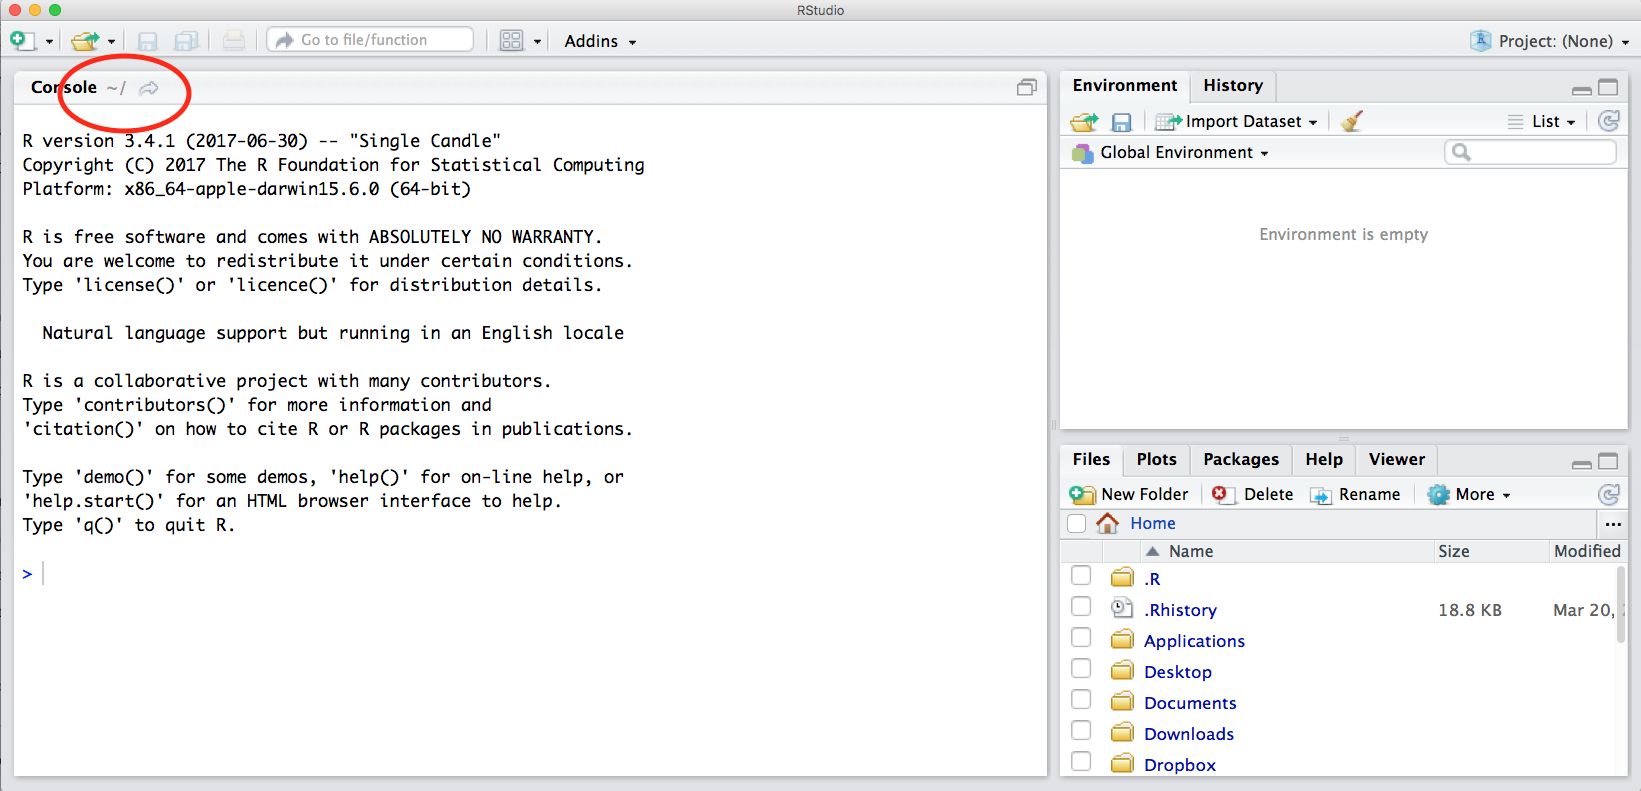
\includegraphics{img/RStudio_IDE_homedir.png}
\caption{}
\end{figure}

OK let's go into the Console, where we interact with the live R process.

Make an assignment and then inspect the object you just created.

\begin{Shaded}
\begin{Highlighting}[]
\NormalTok{x <-}\StringTok{ }\DecValTok{3} \NormalTok{*}\StringTok{ }\DecValTok{4}
\NormalTok{x}
\end{Highlighting}
\end{Shaded}

\begin{verbatim}
## [1] 12
\end{verbatim}

In my head I hear, e.g., ``x gets 12''.

All R statements where you create objects -- ``assignments'' -- have
this form: \texttt{objectName\ \textless{}-\ value}.

I'll write it in the command line with a hashtag \texttt{\#}, which is
the way R comments so it won't be evaluated.

\begin{Shaded}
\begin{Highlighting}[]
\NormalTok{## objectName <- value}

\NormalTok{## This is also how you write notes in your code to explain what you are doing.}
\end{Highlighting}
\end{Shaded}

Object names cannot start with a digit and cannot contain certain other
characters such as a comma or a space. You will be wise to adopt a
\href{http://en.wikipedia.org/wiki/Snake_case}{convention for
demarcating words} in names.

\begin{Shaded}
\begin{Highlighting}[]
\CommentTok{# i_use_snake_case}
\CommentTok{# other.people.use.periods}
\CommentTok{# evenOthersUseCamelCase}
\end{Highlighting}
\end{Shaded}

Make an assignment

\begin{Shaded}
\begin{Highlighting}[]
\NormalTok{this_is_a_really_long_name <-}\StringTok{ }\FloatTok{2.5}
\end{Highlighting}
\end{Shaded}

To inspect this variable, instead of typing it, we can press the up
arrow key and call your command history, with the most recent commands
first. Let's do that, and then delete the assignment:

\begin{Shaded}
\begin{Highlighting}[]
\NormalTok{this_is_a_really_long_name}
\end{Highlighting}
\end{Shaded}

\begin{verbatim}
## [1] 2.5
\end{verbatim}

Another way to inspect this variable is to begin typing
\texttt{this\_}\ldots{}and RStudio will automagically have suggested
completions for you that you can select by hitting the tab key, then
press return.

One more:

\begin{Shaded}
\begin{Highlighting}[]
\NormalTok{science_rocks <-}\StringTok{ }\DecValTok{100}
\end{Highlighting}
\end{Shaded}

Let's try to inspect:

\begin{Shaded}
\begin{Highlighting}[]
\NormalTok{sciencerocks}
\CommentTok{# Error: object 'sciencerocks' not found}
\end{Highlighting}
\end{Shaded}

\subsection{Error messages are your
friends}\label{error-messages-are-your-friends}

Implicit contract with the computer / scripting language: Computer will
do tedious computation for you. In return, you will be completely
precise in your instructions. Typos matter. Case matters. Pay attention
to how you type.

Remember that this is a language, not unsimilar to English! There are
times you aren't understood -- it's going to happen. There are different
ways this can happen. Sometimes you'll get an error. This is like
someone saying `What?' or `Pardon'? Error messages can also be more
useful, like when they say `I didn't understand this specific part of
what you said, I was expecting something else'. That is a great type of
error message. Error messages are your friend. Google them
(copy-and-paste!) to figure out what they mean.

And also know that there are errors that can creep in more subtly, when
you are giving information that is understood, but not in the way you
meant. Like if I'm telling a story about tables and you're picturing
where you eat breakfast and I'm talking about data. This can leave me
thinking I've gotten something across that the listener (or R)
interpreted very differently. And as I continue telling my story you get
more and more confused\ldots{} So write clean code and check your work
as you go to minimize these circumstances!

\subsection{Logical operators and
expressions}\label{logical-operators-and-expressions}

A moment about \textbf{logical operators and expressions}. We can ask
questions about the objects we just made.

\begin{itemize}
\tightlist
\item
  \texttt{==} means `is equal to'
\item
  \texttt{!=} means `is not equal to'
\item
  \texttt{\textless{}} means ` is less than'
\item
  \texttt{\textgreater{}} means ` is greater than'
\item
  \texttt{\textless{}=} means ` is less than or equal to'
\item
  \texttt{\textgreater{}=} means ` is greater than or equal to'
\end{itemize}

\begin{Shaded}
\begin{Highlighting}[]
\NormalTok{science_rocks ==}\StringTok{ }\DecValTok{2}
\end{Highlighting}
\end{Shaded}

\begin{verbatim}
## [1] FALSE
\end{verbatim}

\begin{Shaded}
\begin{Highlighting}[]
\NormalTok{science_rocks <=}\StringTok{ }\DecValTok{30}
\end{Highlighting}
\end{Shaded}

\begin{verbatim}
## [1] FALSE
\end{verbatim}

\begin{Shaded}
\begin{Highlighting}[]
\NormalTok{science_rocks !=}\StringTok{ }\DecValTok{5}
\end{Highlighting}
\end{Shaded}

\begin{verbatim}
## [1] TRUE
\end{verbatim}

\begin{quote}
Shortcuts You will make lots of assignments and the operator
\texttt{\textless{}-} is a pain to type. Don't be lazy and use
\texttt{=}, although it would work, because it will just sow confusion
later. Instead, utilize \textbf{RStudio's keyboard shortcut: Alt + -
(the minus sign)}. Notice that RStudio automagically surrounds
\texttt{\textless{}-} with spaces, which demonstrates a useful code
formatting practice. Code is miserable to read on a good day. Give your
eyes a break and use spaces. RStudio offers many handy
\href{https://support.rstudio.com/hc/en-us/articles/200711853-Keyboard-Shortcuts}{keyboard
shortcuts}. Also, Alt+Shift+K brings up a keyboard shortcut reference
card.
\end{quote}

\begin{quote}
My most common shortcuts include command-Z (undo), and combinations of
arrow keys in combination with shift/option/command (moving quickly up,
down, sideways, with or without highlighting.
\end{quote}

When assigning a value to an object, R does not print anything. You can
force R to print the value by using parentheses or by typing the object
name:

\begin{Shaded}
\begin{Highlighting}[]
\NormalTok{weight_kg <-}\StringTok{ }\DecValTok{55}    \CommentTok{# doesn't print anything}
\NormalTok{(weight_kg <-}\StringTok{ }\DecValTok{55}\NormalTok{)  }\CommentTok{# but putting parenthesis around the call prints the value of `weight_kg`}
\end{Highlighting}
\end{Shaded}

\begin{verbatim}
## [1] 55
\end{verbatim}

\begin{Shaded}
\begin{Highlighting}[]
\NormalTok{weight_kg          }\CommentTok{# and so does typing the name of the object}
\end{Highlighting}
\end{Shaded}

\begin{verbatim}
## [1] 55
\end{verbatim}

Now that R has \texttt{weight\_kg} in memory, we can do arithmetic with
it. For instance, we may want to convert this weight into pounds (weight
in pounds is 2.2 times the weight in kg):

\begin{Shaded}
\begin{Highlighting}[]
\FloatTok{2.2} \NormalTok{*}\StringTok{ }\NormalTok{weight_kg}
\end{Highlighting}
\end{Shaded}

\begin{verbatim}
## [1] 121
\end{verbatim}

We can also change a variable's value by assigning it a new one:

\begin{Shaded}
\begin{Highlighting}[]
\NormalTok{weight_kg <-}\StringTok{ }\FloatTok{57.5}
\FloatTok{2.2} \NormalTok{*}\StringTok{ }\NormalTok{weight_kg}
\end{Highlighting}
\end{Shaded}

\begin{verbatim}
## [1] 126.5
\end{verbatim}

This means that assigning a value to one variable does not change the
values of other variables. For example, let's store the animal's weight
in pounds in a new variable, \texttt{weight\_lb}:

\begin{Shaded}
\begin{Highlighting}[]
\NormalTok{weight_lb <-}\StringTok{ }\FloatTok{2.2} \NormalTok{*}\StringTok{ }\NormalTok{weight_kg}
\end{Highlighting}
\end{Shaded}

and then change \texttt{weight\_kg} to 100.

\begin{Shaded}
\begin{Highlighting}[]
\NormalTok{weight_kg <-}\StringTok{ }\DecValTok{100}
\end{Highlighting}
\end{Shaded}

What do you think is the current content of the object
\texttt{weight\_lb}? 126.5 or 220? Why?

\section{R functions, help pages}\label{r-functions-help-pages}

R has a mind-blowing collection of built-in functions that are used with
the same syntax: function name with parentheses around what the function
needs in order to do what it was built to do. When you type a function
like this, we say we are ``calling the function''.
\texttt{verb(noun\ =\ something,\ adjective\ =\ something,\ etc)}. This
example is from \href{http://r4ds.had.co.nz/pipes}{R for Data Science}
using a children's poem called
\href{https://en.wikipedia.org/wiki/Little_Bunny_Foo_Foo}{Little Bunny
Foo Foo}.

We can call a function without passing it anything (nothing inside the
closed parentheses), and assign it to a variable called
\texttt{foo\_foo}.

\begin{Shaded}
\begin{Highlighting}[]
\NormalTok{## foo_foo <- little_bunny()}
\end{Highlighting}
\end{Shaded}

And since \texttt{foo\_foo} is an object, you can pass it to other
functions:

\begin{Shaded}
\begin{Highlighting}[]
\NormalTok{## hop(foo_foo, through = forest) }
\NormalTok{## scoop(foo_foo, up = field_mice) }
\NormalTok{## bop(foo_foo, on = head)}
\end{Highlighting}
\end{Shaded}

What would happen if I tried to run one of those lines above? I would
get an error because they aren't real functions, and R tells me so:

\begin{Shaded}
\begin{Highlighting}[]
\NormalTok{foo_foo <-}\StringTok{ }\KeywordTok{little_bunny}\NormalTok{()}
\CommentTok{# Error in little_bunny() : could not find function "little_bunny"}
\end{Highlighting}
\end{Shaded}

And that's great, this error message is helpful: R doesn't know what the
\texttt{little\_bunny} function is, and to be honest, neither do we. We
didn't expect that it would know what to do. OK, so now let's look at a
real function.

Let's try using \texttt{seq()} which makes regular sequences of numbers
and, while we're at it, demo more helpful features of RStudio.

Type \texttt{se} and hit TAB. A pop up shows you possible completions.
Specify \texttt{seq()} by typing more to disambiguate or using the
up/down arrows to select. Notice the floating tool-tip-type help that
pops up, reminding you of a function's arguments. If you want even more
help, press F1 as directed to get the full documentation in the help tab
of the lower right pane.

Type the arguments \texttt{1,\ 10} and hit return.

\begin{Shaded}
\begin{Highlighting}[]
\KeywordTok{seq}\NormalTok{(}\DecValTok{1}\NormalTok{, }\DecValTok{10}\NormalTok{)}
\end{Highlighting}
\end{Shaded}

\begin{verbatim}
##  [1]  1  2  3  4  5  6  7  8  9 10
\end{verbatim}

We could probably infer that the \texttt{seq()} function makes a
sequence, but let's learn for sure. Type (and you can autocomplete) and
let's explore the help page:

\begin{Shaded}
\begin{Highlighting}[]
\NormalTok{?seq }
\KeywordTok{help}\NormalTok{(seq) }\CommentTok{# same as ?seq}
\end{Highlighting}
\end{Shaded}

\begin{Shaded}
\begin{Highlighting}[]
\KeywordTok{seq}\NormalTok{(}\DataTypeTok{from =} \DecValTok{1}\NormalTok{, }\DataTypeTok{to =} \DecValTok{10}\NormalTok{) }\CommentTok{# same as seq(1, 10); R assumes by position}
\end{Highlighting}
\end{Shaded}

\begin{verbatim}
##  [1]  1  2  3  4  5  6  7  8  9 10
\end{verbatim}

\begin{Shaded}
\begin{Highlighting}[]
\KeywordTok{seq}\NormalTok{(}\DataTypeTok{from =} \DecValTok{1}\NormalTok{, }\DataTypeTok{to =} \DecValTok{10}\NormalTok{, }\DataTypeTok{by =} \DecValTok{2}\NormalTok{)}
\end{Highlighting}
\end{Shaded}

\begin{verbatim}
## [1] 1 3 5 7 9
\end{verbatim}

The above also demonstrates something about how R resolves function
arguments. You can always specify in \texttt{name\ =\ value} form. But
if you do not, R attempts to resolve by position. So above, it is
assumed that we want a sequence \texttt{from\ =\ 1} that goes
\texttt{to\ =\ 10}. Since we didn't specify step size, the default value
of \texttt{by} in the function definition is used, which ends up being 1
in this case. For functions I call often, I might use this resolve by
position for the first argument or maybe the first two. After that, I
always use \texttt{name\ =\ value}.

The help page tells the name of the package in the top left, and broken
down into sections:

\begin{itemize}
\tightlist
\item
  Description: An extended description of what the function does.
\item
  Usage: The arguments of the function and their default values.
\item
  Arguments: An explanation of the data each argument is expecting.
\item
  Details: Any important details to be aware of.
\item
  Value: The data the function returns.
\item
  See Also: Any related functions you might find useful.
\item
  Examples: Some examples for how to use the function.
\end{itemize}

The examples can be copy-pasted into the console for you to understand
what's going on. Remember we were talking about expecting there to be a
function for something you want to do? Let's try it.

\subsection{Your turn}\label{your-turn}

\begin{quote}
Exercise: Talk to your neighbor(s) and look up the help file for a
function that you know or expect to exist. Here are some ideas:
\texttt{?getwd()}, \texttt{?plot()}, \texttt{min()}, \texttt{max()},
\texttt{?mean()}, \texttt{?log()}).
\end{quote}

And there's also help for when you only sort of remember the function
name: double-questionmark:

\begin{Shaded}
\begin{Highlighting}[]
\NormalTok{??install }
\end{Highlighting}
\end{Shaded}

As we saw with creating the \texttt{foo\_foo} variable above, not all
functions have (or require) arguments:

\begin{Shaded}
\begin{Highlighting}[]
\KeywordTok{date}\NormalTok{()}
\end{Highlighting}
\end{Shaded}

\begin{verbatim}
## [1] "Tue Nov 21 16:44:32 2017"
\end{verbatim}

\section{Clearing the environment}\label{clearing-the-environment}

Now look at the objects in your environment (workspace) -- in the upper
right pane. The workspace is where user-defined objects accumulate.

\begin{figure}[htbp]
\centering
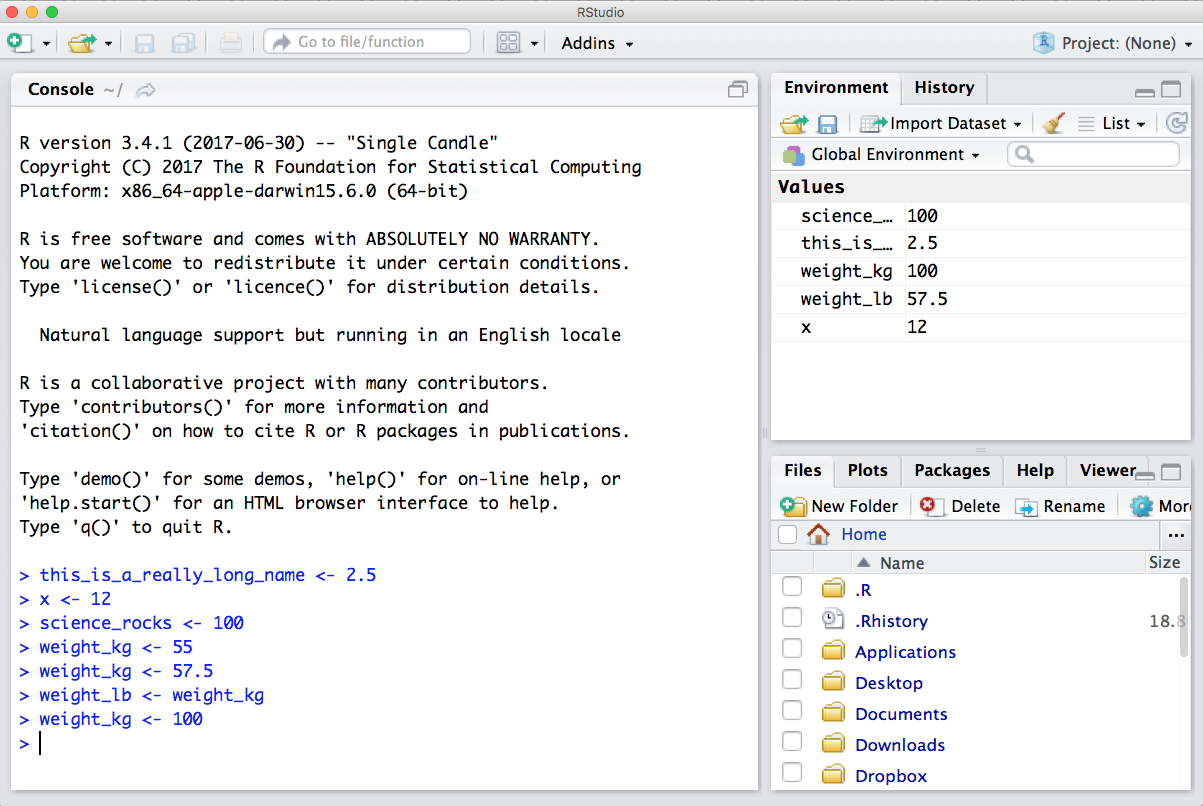
\includegraphics{img/RStudio_IDE_env.png}
\caption{}
\end{figure}

You can also get a listing of these objects with a few different R
commands:

\begin{Shaded}
\begin{Highlighting}[]
\KeywordTok{objects}\NormalTok{()}
\end{Highlighting}
\end{Shaded}

\begin{verbatim}
## [1] "science_rocks"              "this_is_a_really_long_name"
## [3] "weight_kg"                  "weight_lb"                 
## [5] "x"
\end{verbatim}

\begin{Shaded}
\begin{Highlighting}[]
\KeywordTok{ls}\NormalTok{()}
\end{Highlighting}
\end{Shaded}

\begin{verbatim}
## [1] "science_rocks"              "this_is_a_really_long_name"
## [3] "weight_kg"                  "weight_lb"                 
## [5] "x"
\end{verbatim}

If you want to remove the object named \texttt{weight\_kg}, you can do
this:

\begin{Shaded}
\begin{Highlighting}[]
\KeywordTok{rm}\NormalTok{(weight_kg)}
\end{Highlighting}
\end{Shaded}

To remove everything:

\begin{Shaded}
\begin{Highlighting}[]
\KeywordTok{rm}\NormalTok{(}\DataTypeTok{list =} \KeywordTok{ls}\NormalTok{())}
\end{Highlighting}
\end{Shaded}

or click the broom in RStudio's Environment pane.

\subsection{Your turn}\label{your-turn-1}

\begin{quote}
Exercise: Clear your workspace, then create a few new variables. Create
a variable that is the mean of a sequence of 1-20. What's a good name
for your variable? Does it matter what your `by' argument is? Why?
\end{quote}

\section{RMarkdown}\label{rmarkdown}

Now we are going to also introduce RMarkdown. This is really key for
collaborative research, so we're going to get started with it early and
then use it for the rest of the day.

An Rmarkdown file will allow us to weave markdown text with chunks of R
code to be evaluated and output content like tables and plots.

File -\textgreater{} New File -\textgreater{} Rmarkdown\ldots{}
-\textgreater{} Document of output format HTML, OK.

You can give it a Title like ``My Project''. Then click OK.

OK, first off: by opening a file, we are seeing the 4th pane of the
RStudio console, which is essentially a text editor. This lets us
organize our files within RStudio instead of having a bunch of differnt
windows open.

Let's have a look at this file --- it's not blank; there is some initial
text is already provided for you. Notice a few things about it:

\begin{itemize}
\tightlist
\item
  There are white and grey sections. R code is in grey sections, and
  other text is in white.
\end{itemize}

\begin{figure}[htbp]
\centering
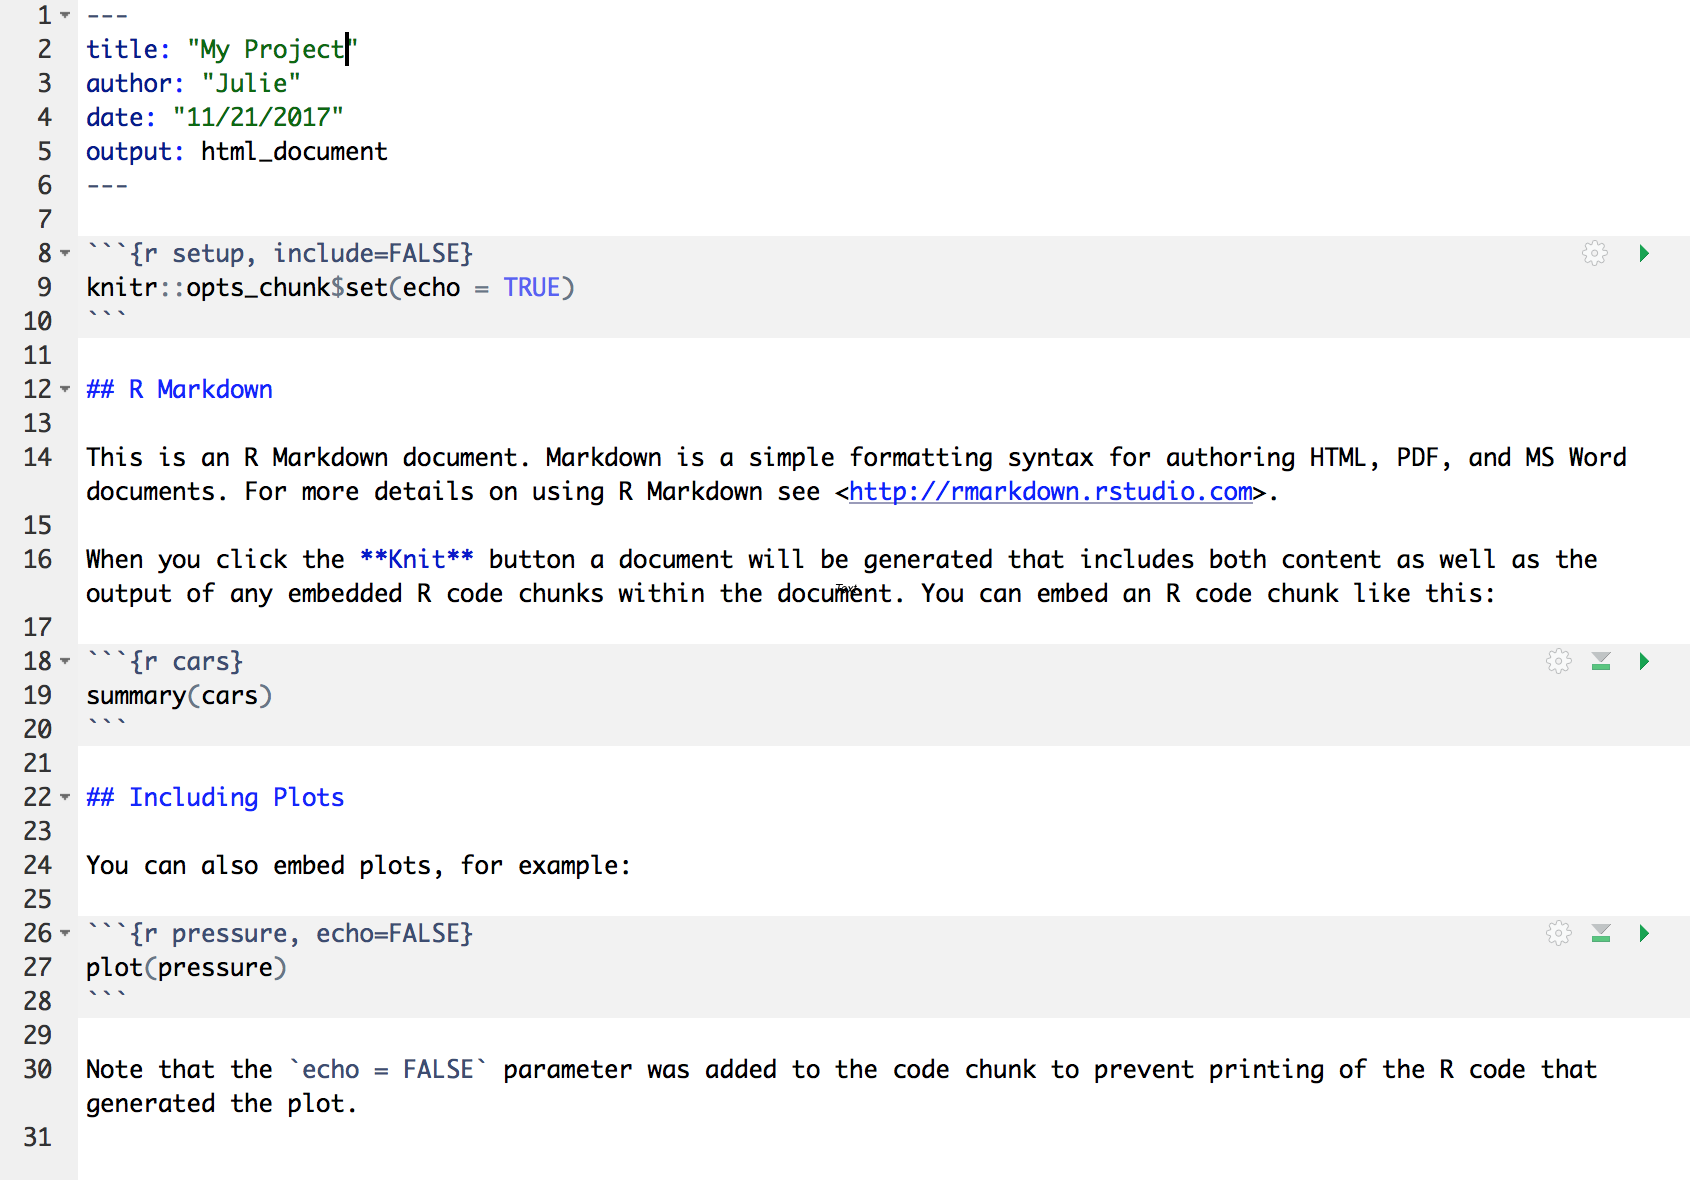
\includegraphics{img/rmarkdown.png}
\caption{}
\end{figure}

Let's go ahead and ``Knit HTML''.

\begin{figure}[htbp]
\centering
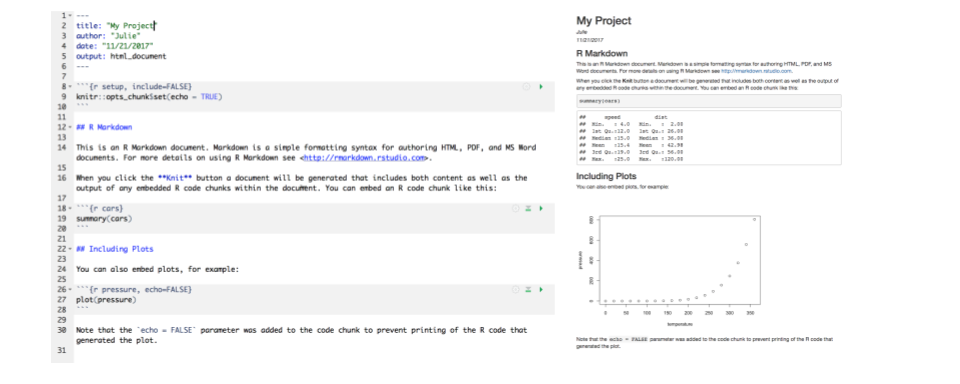
\includegraphics{img/rmarkdown_side_by_side.png}
\caption{}
\end{figure}

What do you notice between the two?

Notice how the grey \textbf{R code chunks} are surrounded by 3 backticks
and \texttt{\{r\ LABEL\}}. These are evaluated and return the output
text in the case of \texttt{summary(cars)} and the output plot in the
case of \texttt{plot(pressure)}.

Notice how the code \texttt{plot(pressure)} is not shown in the HTML
output because of the R code chunk option \texttt{echo=FALSE}.

More details\ldots{}

This RMarkdown file has 2 different languages within it: \textbf{R} and
\textbf{Markdown}.

We don't know that much R yet, but you can see that we are taking a
summary of some data called `cars', and then plotting. There's a lot
more to learn about R, and we'll get into it for the next few days.

The second language is Markdown. This is a formatting language for plain
text, and there are only about 15 rules to know.

Notice the syntax for:

\begin{itemize}
\tightlist
\item
  \textbf{headers} get rendered at multiple levels: \texttt{\#},
  \texttt{\#\#}
\item
  \textbf{bold}: \texttt{**word**}
\end{itemize}

There are some good
\href{https://github.com/adam-p/markdown-here/wiki/Markdown-Here-Cheatsheet}{cheatsheets}
to get you started, and here is one built into RStudio:

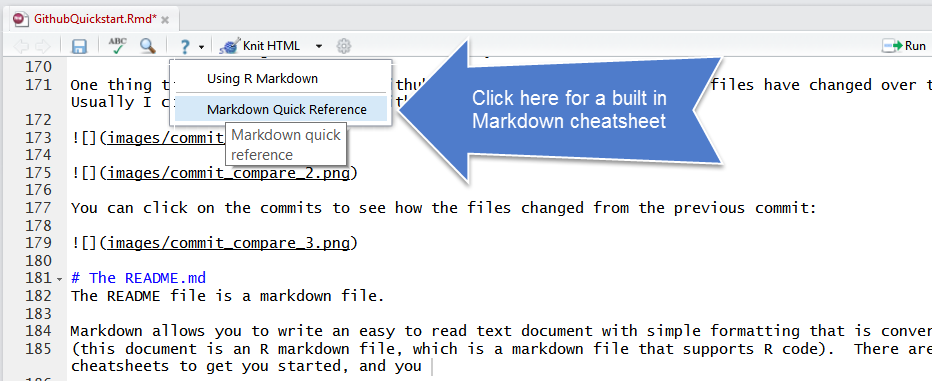
\includegraphics{img/md_cheatsheet.png}

See
\href{https://guides.github.com/features/mastering-markdown/}{Mastering
Markdown · GitHub Guides} and add some more personalized content to the
README of your own, like a bulleted list or blockquote.

Learn more: \url{http://rmarkdown.rstudio.com/}

\subsection{Your Turn}\label{your-turn-2}

\begin{enumerate}
\def\labelenumi{\arabic{enumi}.}
\tightlist
\item
  In Markdown, Write some italic text, and make a numbered list. Use the
  Markdown Quick Reference (in the menu bar: Help \textgreater{}
  Markdown Quick Reference).
\item
  Reknit your html file.
\end{enumerate}

\section{Setup Git \& GitHub}\label{setup-git-github}

We're going to switch gears from R for a moment and set up Git and
GitHub, which we will be using along with R and RStudio for the rest of
the workshop. This set up is a one-time thing! You will only have to do
this once per computer. We'll walk through this together.

\begin{enumerate}
\def\labelenumi{\arabic{enumi}.}
\item
  Create \textbf{Github} account at \url{http://github.com}, if you
  don't already have one. For username, I recommend all lower-case
  letters, short as you can. I recommend using your \emph{.edu email},
  since you can request free private repositories via
  \href{https://education.github.com/}{GitHub Education} discount.
\item
  Configure \textbf{git} with global commands, which means it will apply
  `globally' to all files on your computer, rather than to a specific
  folder. Open the Git Bash program (Windows) or the Terminal (Mac) and
  type the following:

\begin{verbatim}
# display your version of git
git --version

# replace USER with your Github user account
git config –-global user.name USER

# replace NAME@EMAIL.EDU with the email you used to register with Github
git config –-global user.email NAME@EMAIL.EDU

# list your config to confirm user.* variables set
git config --list
\end{verbatim}
\end{enumerate}

Not only have you just set up git as a one-time-only thing, you have
just used the command line. We don't have time to learn much of the
command line today, but you just successfully used it following explicit
instructions, which is huge! There are great resources for learning the
command line, check out
\href{http://remi-daigle.github.io/2016-04-15-UCSB/shell/}{this tutorial
from SWC at UCSB}.

\section{Troubleshooting}\label{troubleshooting}

Here are some additional things we didn't have time to discuss:

\subsection{I just entered a command and nothing's
happening}\label{i-just-entered-a-command-and-nothings-happening}

It may be because you didn't complete a command: is there a little
\texttt{+} in your console? R is saying that it is waiting for you to
finish. In the example below, I need to close that parenthesis.

\begin{Shaded}
\begin{Highlighting}[]
\NormalTok{>}\StringTok{ }\NormalTok{x <-}\StringTok{ }\KeywordTok{seq}\NormalTok{(}\DecValTok{1}\NormalTok{, }\DecValTok{10}
\NormalTok{+}\StringTok{ }
\end{Highlighting}
\end{Shaded}

\subsection{How do I update RStudio?}\label{how-do-i-update-rstudio}

To see if you have the most current version of RStudio, go to the Help
bar \textgreater{} Check for Updates. If there is an update available,
you'll have the option to Quit and Download, which will take you to
\url{http://www.rstudio.com/download}. When you download and install,
choose to replace the previous version.

\chapter{Using RStudio+GitHub, and R Scripts}\label{rstudio-github}

We will learn about version control using git and GitHub, and we will
interface with this through RStudio.

git will track and version your files, GitHub stores this online and
enables you to collaborate with others (and yourself). Although git and
GitHub are two different things, distinct from each other, I think of
them as a bundle since I always use them together. It also helped me to
think of GitHub like Dropbox: you make folders that are `tracked' and
can be synced to the cloud. GitHub does this too, but you have to be
more deliberate about when syncs are made. This is because GitHub saves
these as different versions, with information about who contributed
when, line-by-line. This makes collaboration easier, and it allows you
to roll-back to different versions or contribute to others' work.

\section{Objectives \& Resources}\label{objectives-resources-1}

\subsubsection{Objectives}\label{objectives}

Today, we'll interface with GitHub from our local computers using
RStudio. There are many other ways to interact with GitHub, including
GitHub's Desktop App or the command line
(\href{http://stat545.com/git02_git-clients.html}{here is Jenny Bryan's
list of git clients}), but today we are going to work from RStudio. You
have the largest suite of options if you interface through the command
line, but the most common things you'll do can be done through one of
these other applications (i.e.~RStudio and the GitHub Desktop App).

Here's what we'll do (we already set up git on our local computer in the
previous section):

\begin{enumerate}
\def\labelenumi{\arabic{enumi}.}
\tightlist
\item
  create a repository on Github.com
\item
  clone locally using RStudio
\item
  learn the RStudio-GitHub workflow by syncing to Github.com: pull,
  stage, commit, push
\item
  explore github.com: files, commit history, file history
\item
  create an R script
\item
  practice the RStudio-GitHub workflow by editing and adding files
\end{enumerate}

\subsubsection{Resources}\label{resources}

These materials borrow from:

\begin{itemize}
\tightlist
\item
  Jenny Bryan's lectures from STAT545 at UBC:
  \href{http://stat545.com/git09_shell.html}{The Shell}
\item
  Jenny Bryan's \href{http://happygitwithr.com}{Happy git with R}
  tutorial
\item
  Melanie Frazier's
  \href{https://rawgit.com/nazrug/Quickstart/master/GithubQuickstart.html}{GitHub
  Quickstart}
\item
  Ben Best's
  \href{http://remi-daigle.github.io/2016-04-15-UCSB/git/}{Software
  Carpentry at UCSB}
\end{itemize}

Today, we'll only introduce the features and terminology that scientists
need to learn to begin managing their projects.

\section{Why should scientists use
Github?}\label{why-should-scientists-use-github}

\begin{enumerate}
\def\labelenumi{\arabic{enumi}.}
\tightlist
\item
  Ends (or, nearly ends) the horror of keeping track of versions.
  Basically, we get away from this: 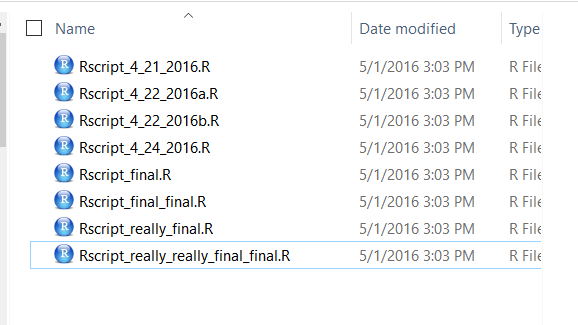
\includegraphics{img/MessySaves.png}
  When you open your repository, you only see the most recent version.
  But, it easy to compare versions, and you can easily revert to
  previous versions. 
\item
  Improves collaborative efforts. Different researchers can work on the
  same files at the same time!
\item
  It is easy to share and distribute files through the Github website.
\item
  Your files are available anywhere, you just need internet connection!
\end{enumerate}

\subsection{What are Git and Github?}\label{what-are-git-and-github}

\begin{itemize}
\item
  \textbf{Git} is a version control system that lets you track changes
  to files over time. These files can be any kind of file (eg .doc,
  .pdf, .xls), but free text differences are most easily visible (eg
  txt, csv, md).
\item
  \textbf{Github} is a website for storing your git versioned files
  remotely. It has many nice features to be able visualize differences
  between
  \href{https://help.github.com/articles/rendering-and-diffing-images/}{images},
  \href{https://help.github.com/articles/mapping-geojson-files-on-github/}{rendering}
  \&
  \href{https://github.com/blog/1772-diffable-more-customizable-maps}{diffing}
  map data files,
  \href{https://help.github.com/articles/rendering-csv-and-tsv-data/}{render
  text data files}, and
  \href{https://help.github.com/articles/rendering-differences-in-prose-documents/}{track
  changes in text}.
\end{itemize}

\begin{quote}
If you are a student you can get the micro account which includes 5
private repositories for free (normally a \$7/month value). You can sign
up for the student account
\href{https://education.github.com/pack}{here}. Instructors can also
request a free organization
\href{https://education.github.com/}{account, ``Request a discount''}.
\end{quote}

Github was developed for social coding (i.e., sort of like an open
source Wikipedia for programmers). Consequently, much of the
functionality and terminology of Github (e.g., branches and pull
requests) isn't necessary for a scientist getting started.

These concepts are more important for coders who want the entire coding
community (and not just people working on the same project) to be able
to suggest changes to their code. This isn't how most scientists will
use Github.

To get the full functionality of Github, you will eventually want to
learn other concepts. But, this can wait.

\subsection{Some Github terminology}\label{some-github-terminology}

\begin{itemize}
\tightlist
\item
  \textbf{User}: A Github account for you (e.g., jules32).
\item
  \textbf{Organization}: The Github account for one or more user (e.g.,
  datacarpentry).
\item
  \textbf{Repository}: A folder within the organization that includes
  files dedicated to a project.
\item
  \textbf{Local Github}: Copies of Github files located your computer.
\item
  \textbf{Remote Github}: Github files located on the
  \url{https://github.com} website.
\item
  \textbf{Clone}: Process of making a local copy of a remote Github
  repository. This only needs to be done once (unless you mess up your
  local copy).
\item
  \textbf{Pull}: Copy changes on the remote Github repository to your
  local Github repository. This is useful if multiple people are making
  changes to a repository.
\item
  \textbf{Push}: Save local changes to remote Github 
\end{itemize}

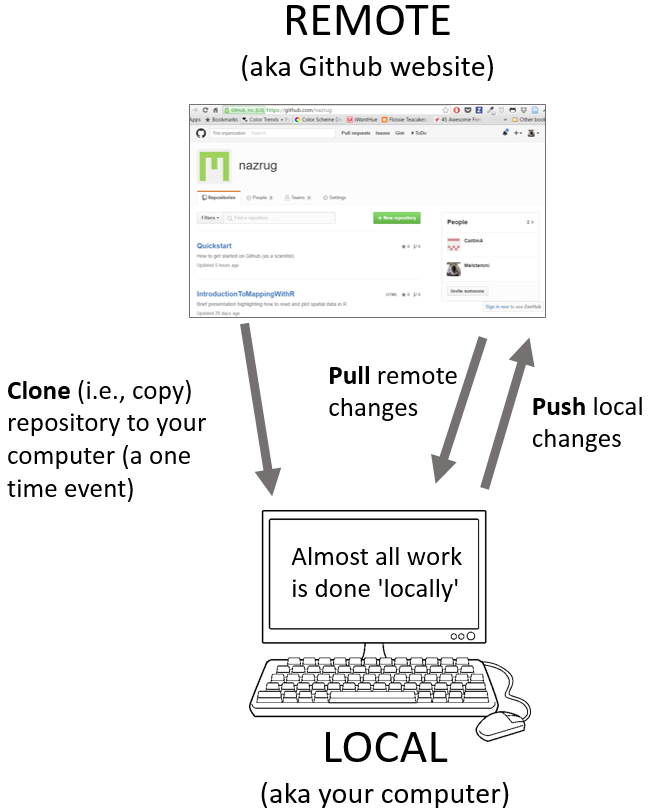
\includegraphics{img/push_pull_clone.png}

\section{Create a repository on
Github.com}\label{create-a-repository-on-github.com}

First, go to your account on github.com and click ``New repository''.
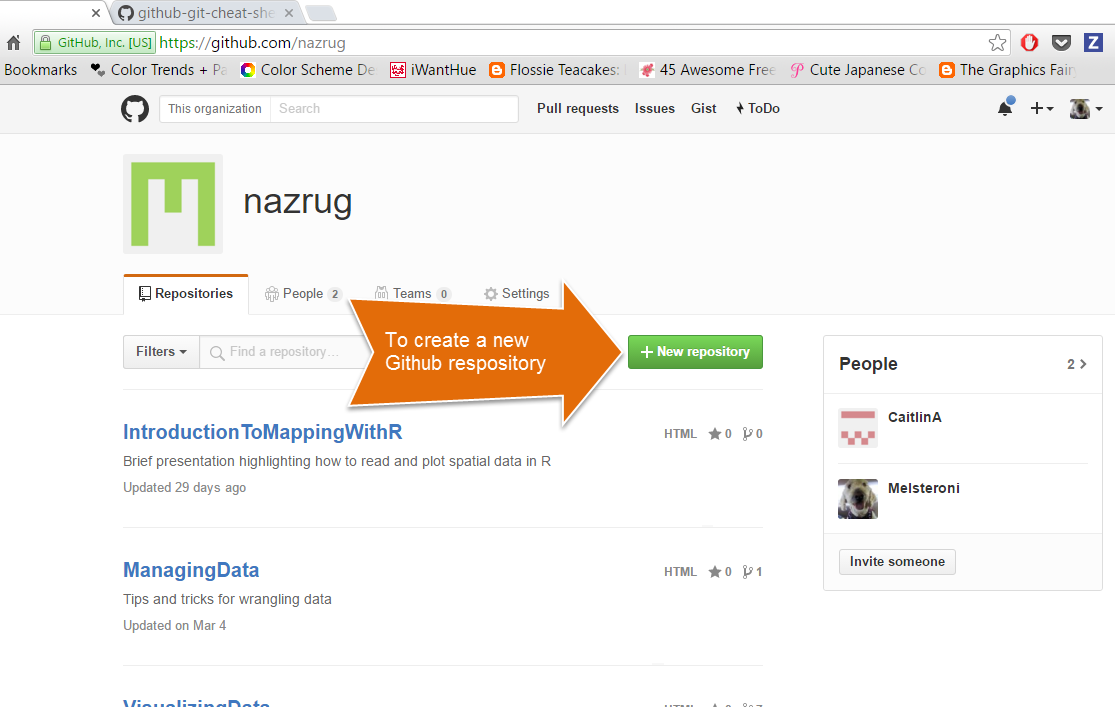
\includegraphics{img/create_repository.png}

Choose a name.Call it whatever you want (the shorter the better), or
follow me for convenience. I will call mine \texttt{my-repo}.

Also, add a description, make it public, create a README file, and
create your repo! 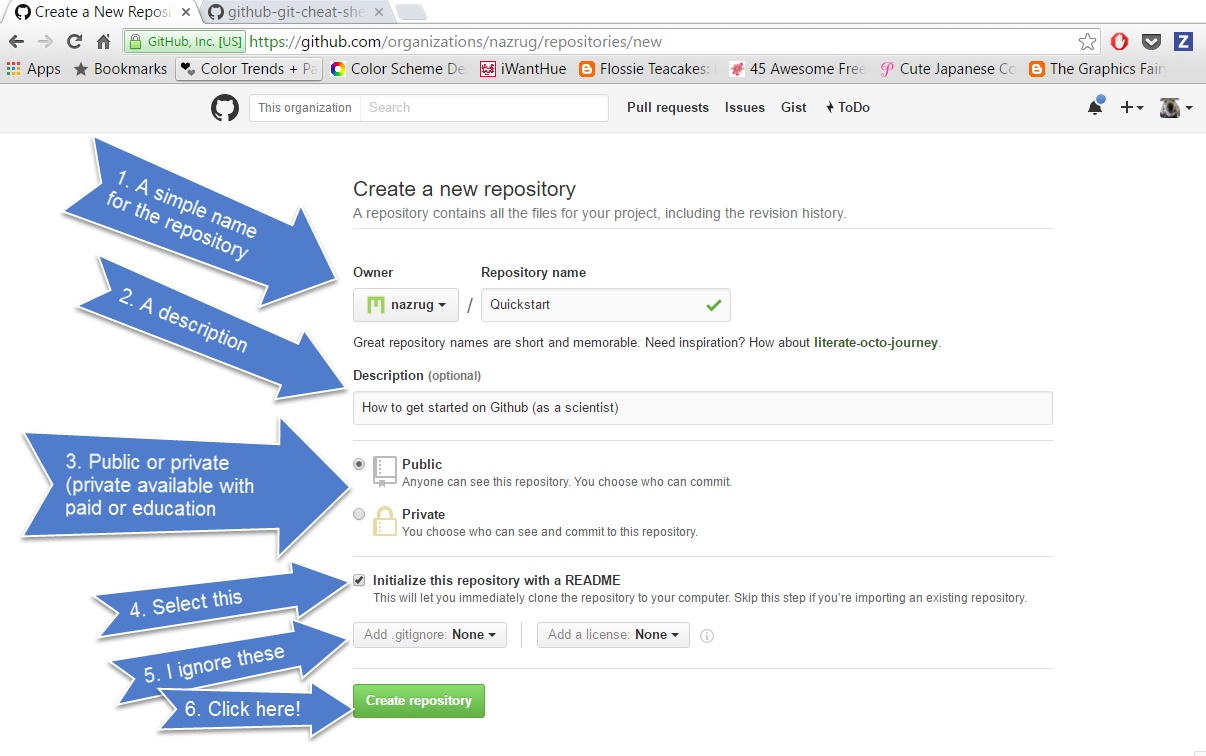
\includegraphics{img/create_repository_2.png}

The \emph{Add gitignore} option adds a document where you can identify
files or file-types you want Github to ignore. These files will stay in
on the local Github folder (the one on your computer), but will not be
uploaded onto the web version of Github.

The \emph{Add a license} option adds a license that describes how other
people can use your Github files (e.g., open source, but no one can
profit from them, etc.). We won't worry about this today.

Check out our new repository!

Notice how the README.md file we created is automatically displayed at
the bottom.

\includegraphics{img/new_repository.png}

\textbf{From here, you will work locally (on your computer).}

\section{Clone your repository using
RStudio}\label{clone-your-repository-using-rstudio}

We'll start of by cloning to our local computer using RStudio. We are
going to be cloning a copy of our Remote repository on Github.com to our
local computers. Unlike downloading, cloning keeps all the version
control and user information bundled with the files.

\textbf{Step 0}: Create your \texttt{github} folder

This is really important! We need to be organized and deliberate about
where we want to keep all of our GitHub repositories (since this is the
first of many in your career).

Let's all make a folder called \texttt{github} (all lowercase!) in our
home directories. So it will look like this:

\begin{itemize}
\tightlist
\item
  Windows:
  \texttt{Users\textbackslash{}{[}User{]}\textbackslash{}Documents\textbackslash{}github\textbackslash{}}
\item
  Mac: \texttt{Users/{[}User{]}/github/}
\end{itemize}

This will let us take advantage of something that is really key about
GitHub.com: you can easily navigate through folders within repositories
and the urls reflect this navigation. The greatness of this will be
evident soon. So let's set ourselves up for easily translating (and
remembering) those navigation paths by having a folder called
\texttt{github} that will serve as our `github.com'.

So really. Make sure that you have an all-lowercase folder called
\texttt{github} in your home directory!!

\textbf{Step 1}: Copy the web address of the repository you want to
clone.

\begin{figure}[htbp]
\centering
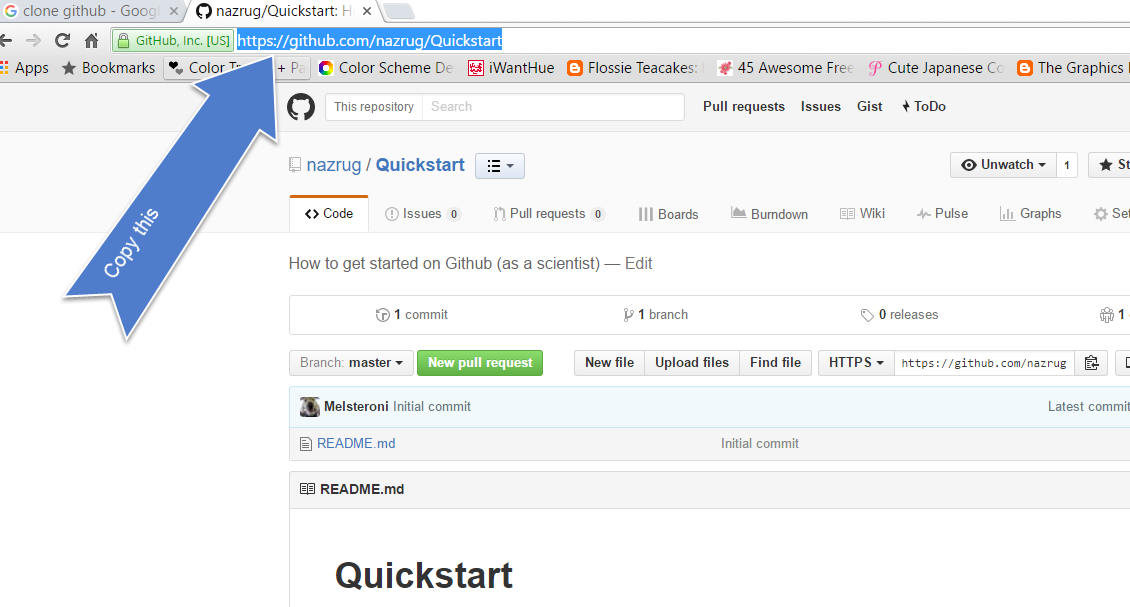
\includegraphics{img/clone_step1.png}
\caption{}
\end{figure}

\textbf{Step 2}: from RStudio, go to New Project (also in the File
menu).

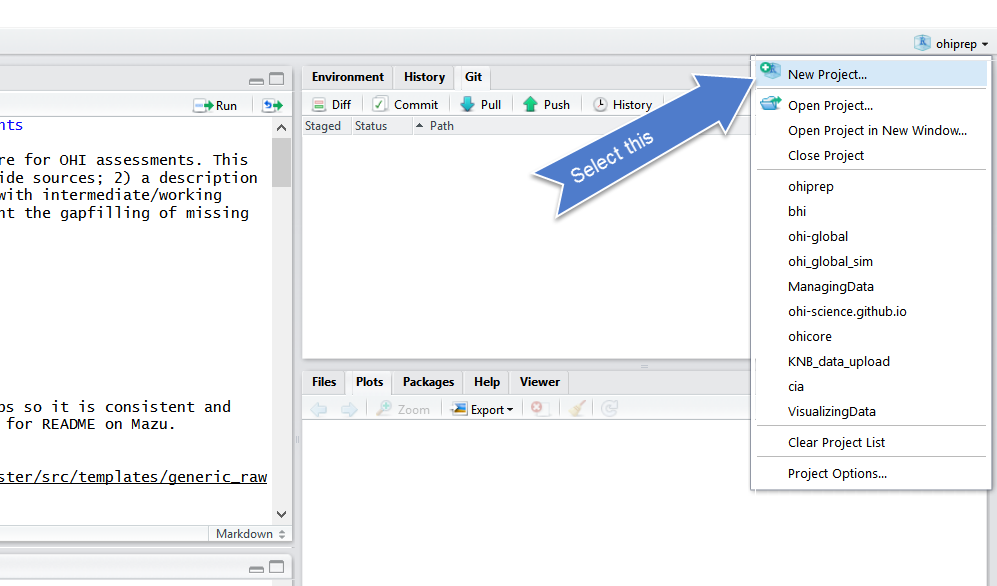
\includegraphics{img/new_project_1.png}

\textbf{Step 3}: Select Version Control

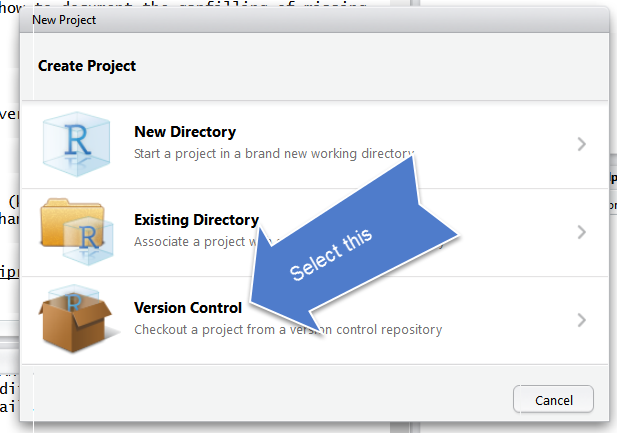
\includegraphics{img/new_project_2.png}

\textbf{Step 4}: Select Git

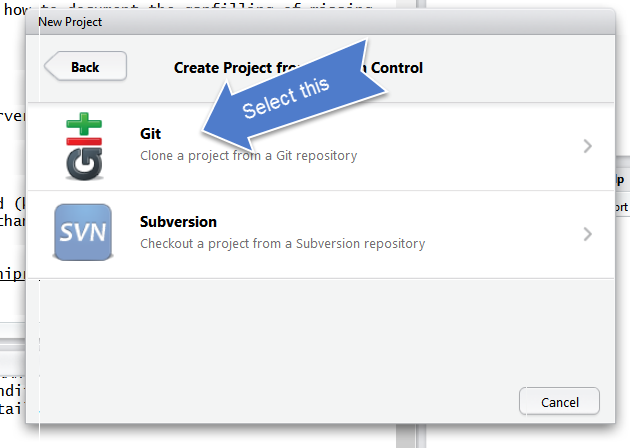
\includegraphics{img/new_project_3.png}

\textbf{Step 5}: Paste it in the Repository URL field, and type tab to
autofill the Project Directory name. Make sure you keep the Project
Directory Name THE SAME as the repository name from the URL.

Save it in your github folder (click on Browse) to do this.

\begin{figure}[htbp]
\centering
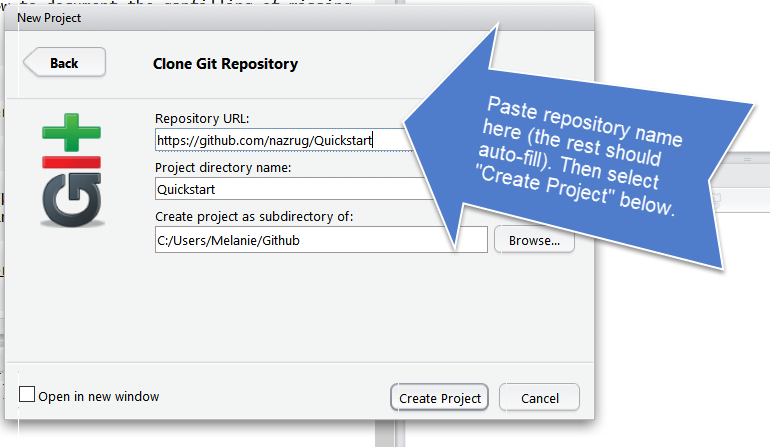
\includegraphics{img/new_project_4.png}
\caption{}
\end{figure}

If everything went well, the repository will be added to the list
located here: 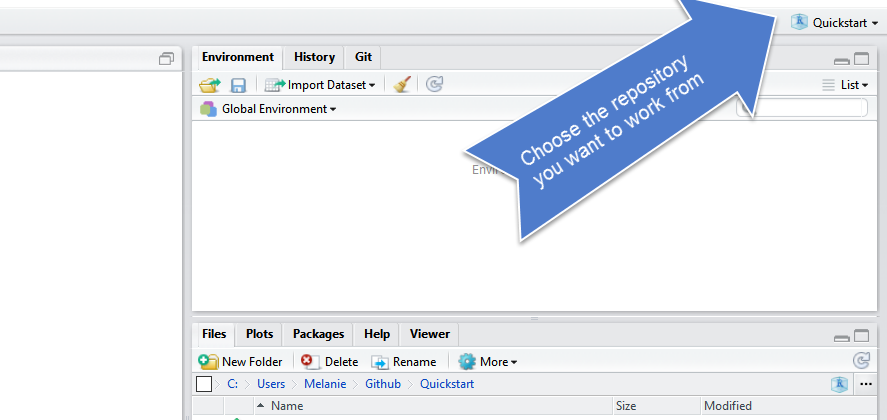
\includegraphics{img/select_project.png}

And the repository will be saved to the Github folder on your computer:

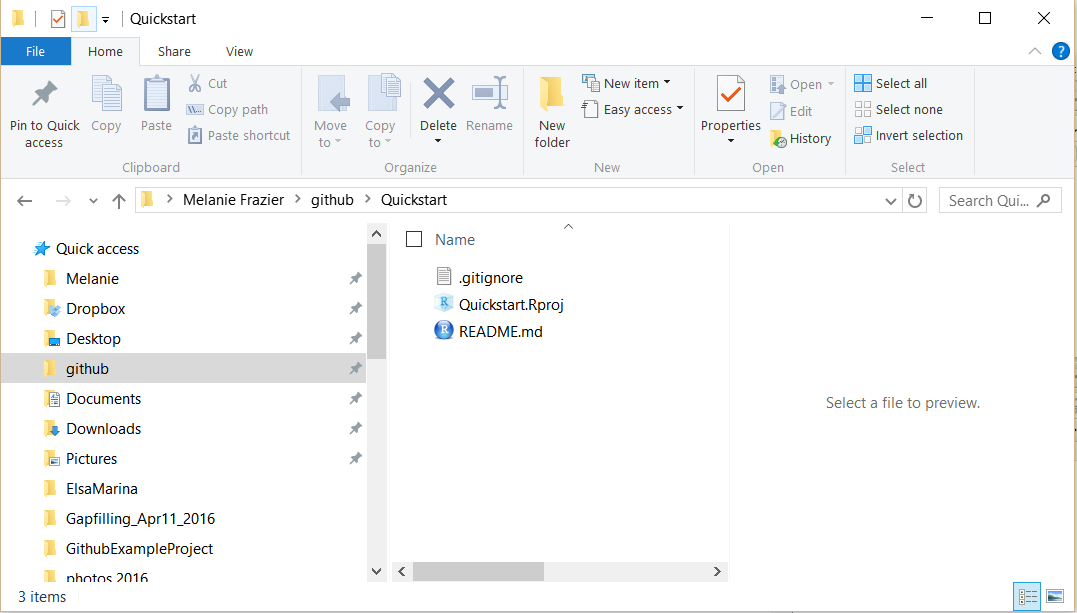
\includegraphics{img/cloned_repository.png}

Ta da!!!! The folder doesn't contain much of interest, but we are going
to change that.

\section{Inspect your repository}\label{inspect-your-repository}

Notice a few things in our repo here:

\begin{enumerate}
\def\labelenumi{\arabic{enumi}.}
\tightlist
\item
  Our working directory is set to
  \texttt{\textasciitilde{}/github/my-repo}. This means that I can start
  working with the files I have in here without setting the filepath.
  This is that when we cloned this from RStudio, it created an RStudio
  project, which you can tell because:

  \begin{itemize}
  \tightlist
  \item
    \texttt{.RProj} file, which you can see in the Files pane.
  \item
    The project is named in the top right hand corner
  \end{itemize}
\item
  We have a git tab! This is how we will interface directly to
  Github.com
\end{enumerate}

\begin{figure}[htbp]
\centering
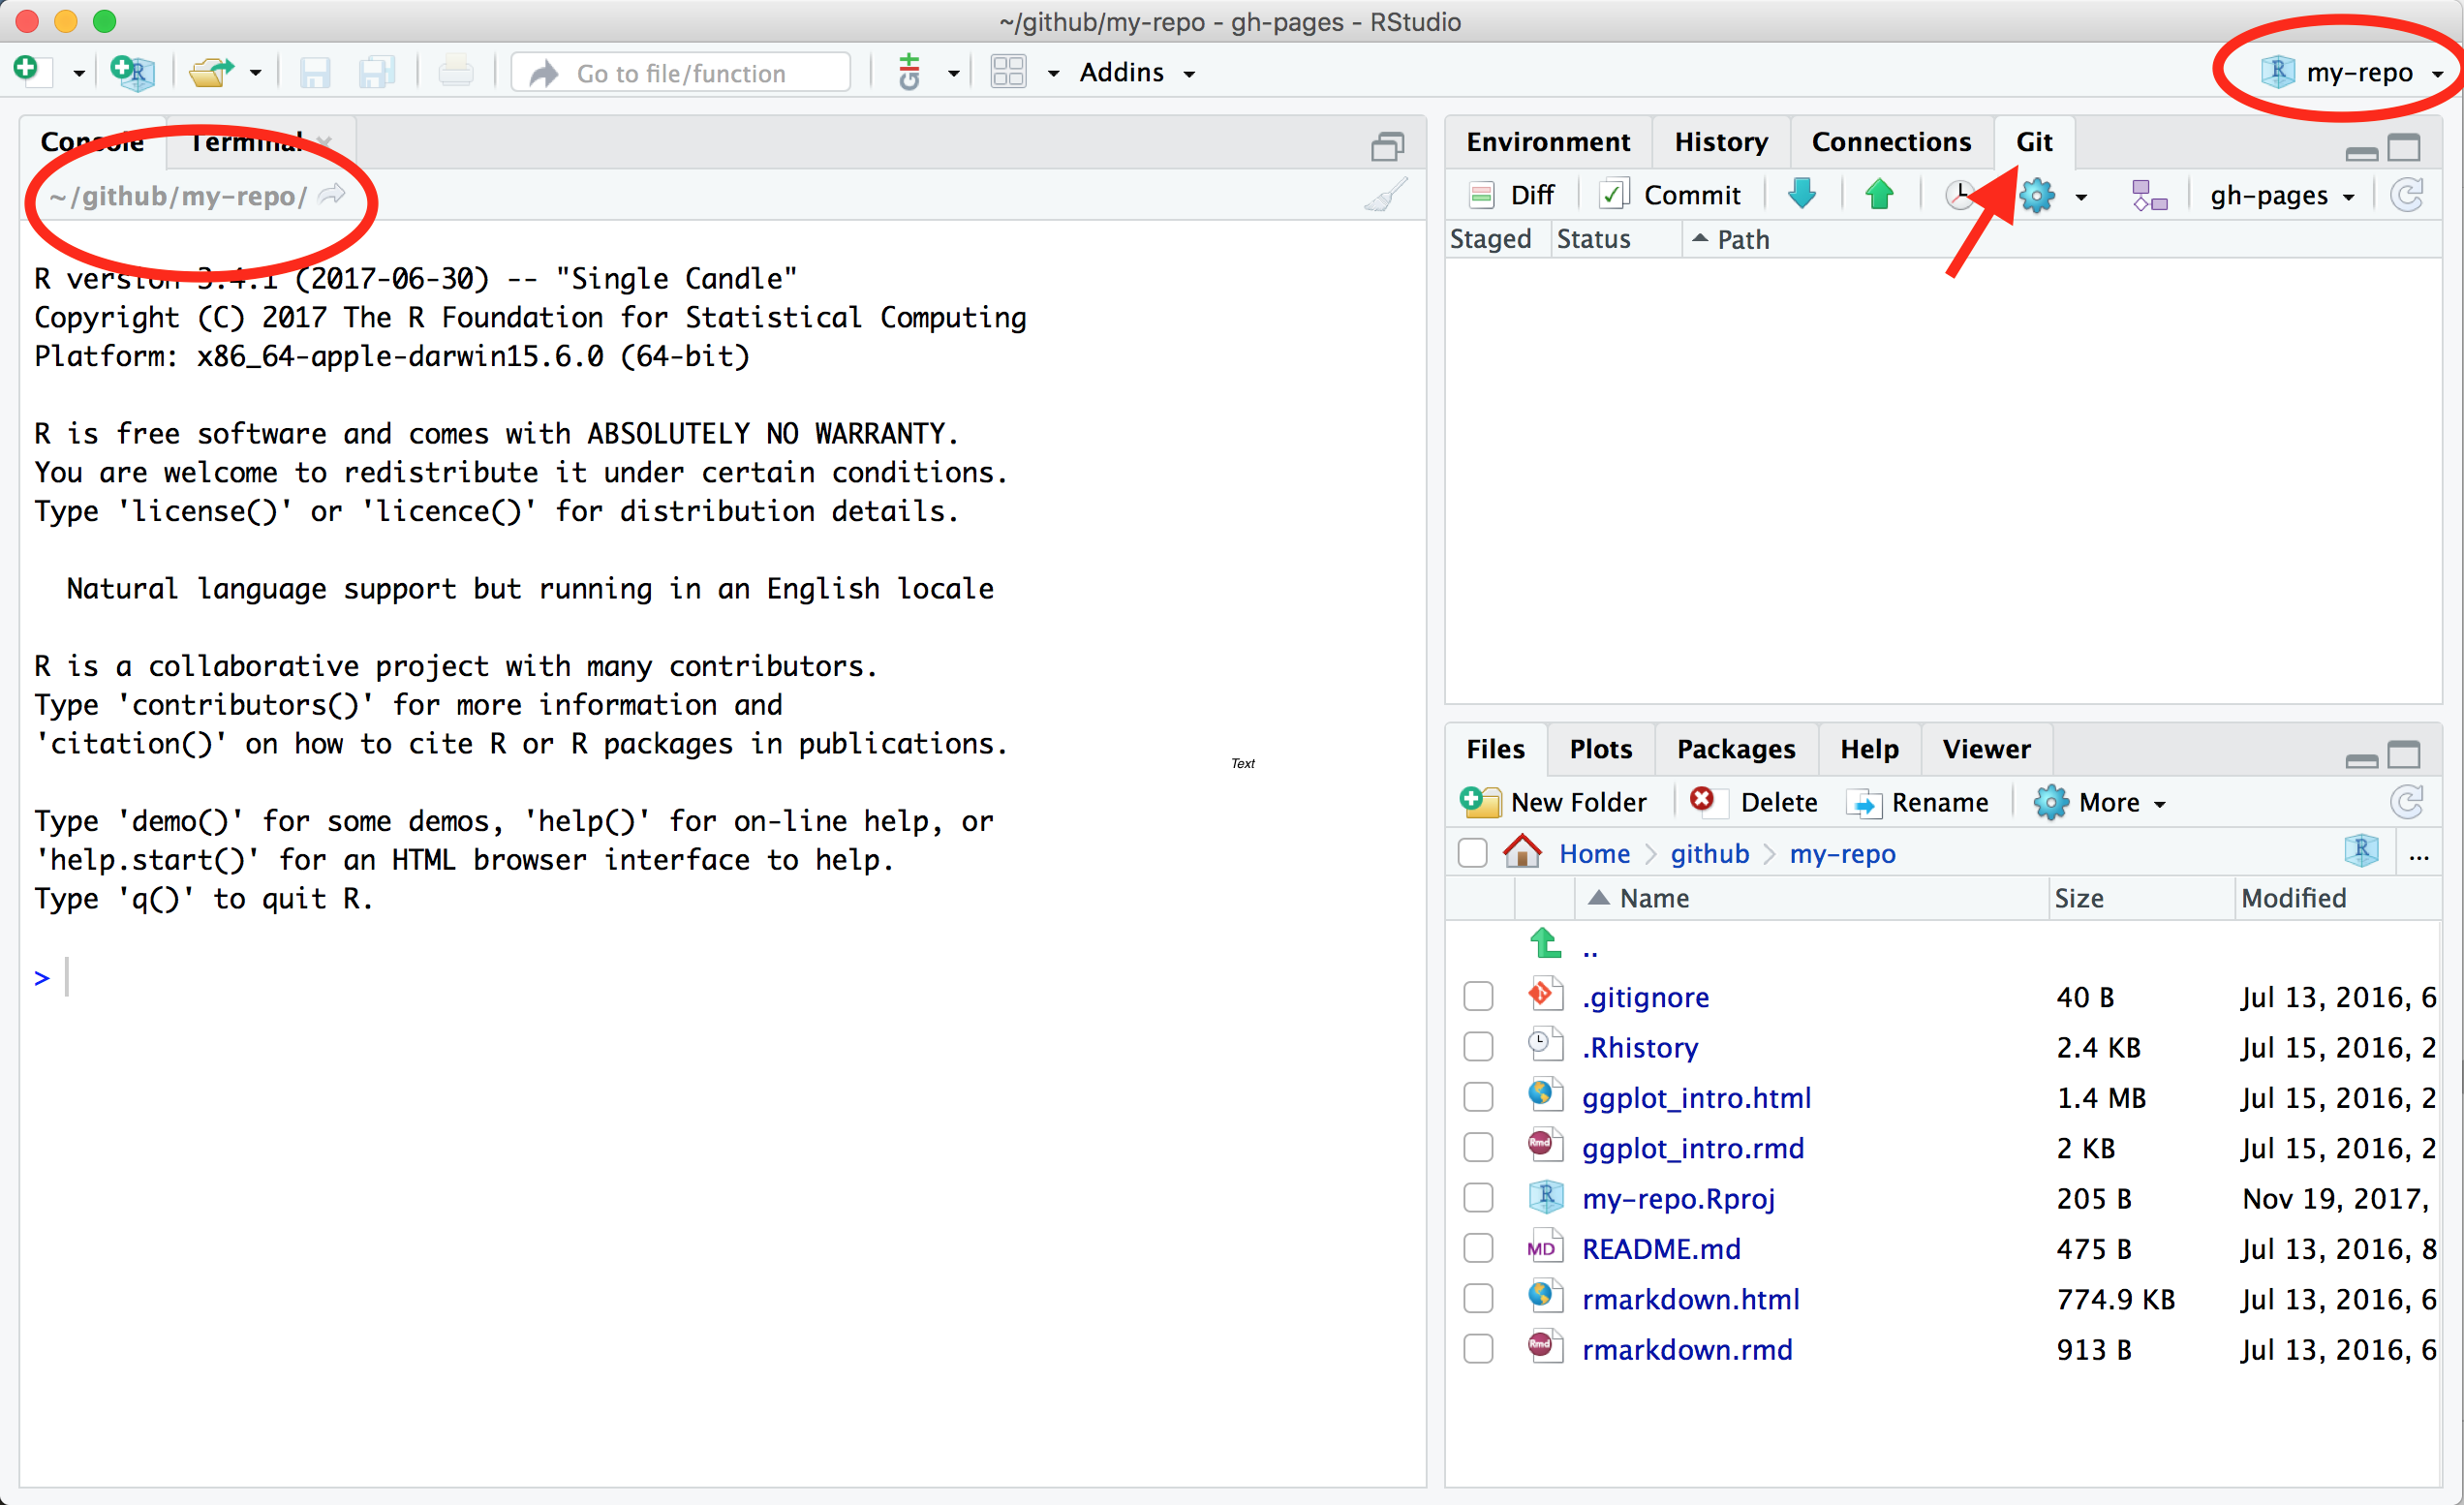
\includegraphics{img/RStudio_IDE_git.png}
\caption{}
\end{figure}

\section{Add files to our local repo}\label{add-files-to-our-local-repo}

The repository will contain:

\begin{itemize}
\tightlist
\item
  .gitignore file
\item
  README.md
\item
  Rproj
\end{itemize}

And, I typically create the following:

\begin{itemize}
\tightlist
\item
  folders for ``data'' and ``figures''\\
\item
  R scripts
\item
  etc.
\end{itemize}

I'm going to copy-paste a small from my desktop into the folder.

To make changes to the repository, you will work from your computer
(``local Github'').

When files are changed in the local repository, these changes will be
reflected in the Git tab of RStudio:

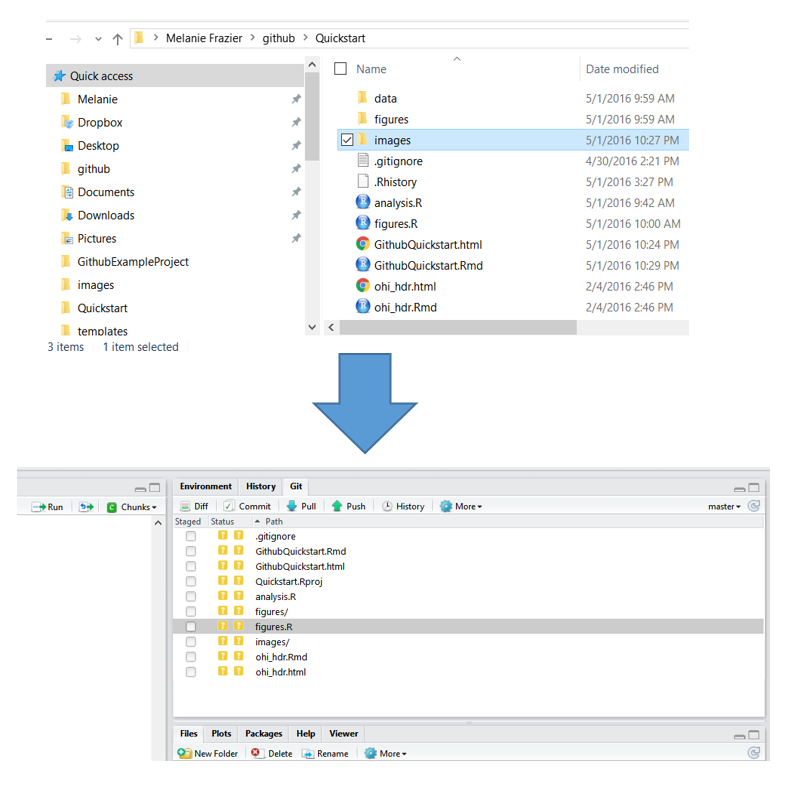
\includegraphics{img/modify_files.png}

\subsection{Inspect what has changed}\label{inspect-what-has-changed}

These are the codes RStudio uses to describe how the files are changed,
(from the RStudio
\href{http://www.rstudio.com/wp-content/uploads/2016/01/rstudio-IDE-cheatsheet.pdf}{cheatsheet}):
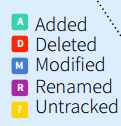
\includegraphics{img/modified.png}

\section{Sync from RStudio to GitHub}\label{sync-from-rstudio-to-github}

When you are ready to commit your changes, you follow these steps:

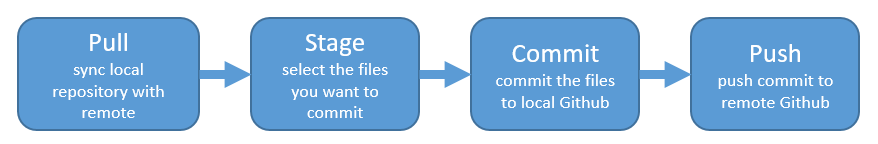
\includegraphics{img/commit_overview.png}

We walk through this process below:

\subsection{Pull}\label{pull}

From the Git tab, ``Pull'' the repository. This makes sure your local
repository is synced with the remote repository. This is very important
if other people are making changes to the repository or if you are
working from multiple computers.

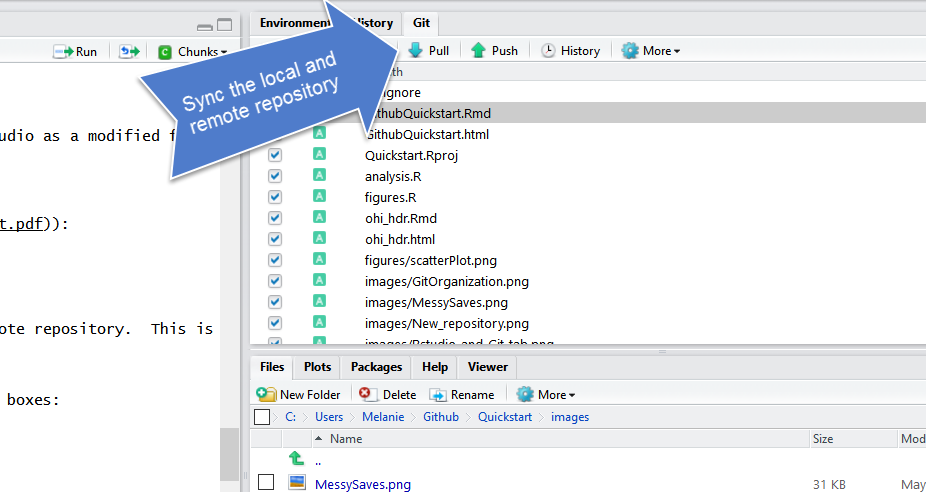
\includegraphics{img/pull.png}

\subsection{Stage}\label{stage}

Stage the files you want to commit. In RStudio, this involves checking
the ``Staged'' boxes:

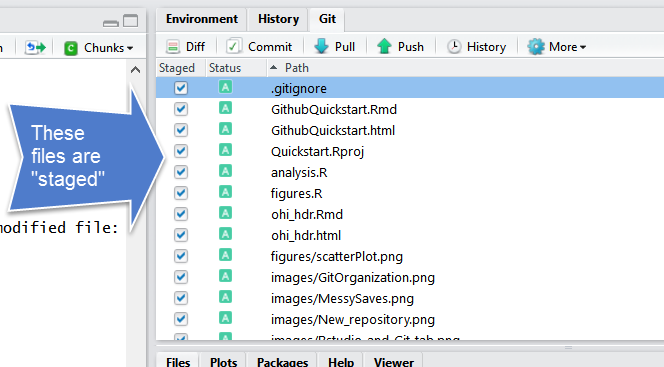
\includegraphics{img/staged.png}

\subsection{Commit}\label{commit}

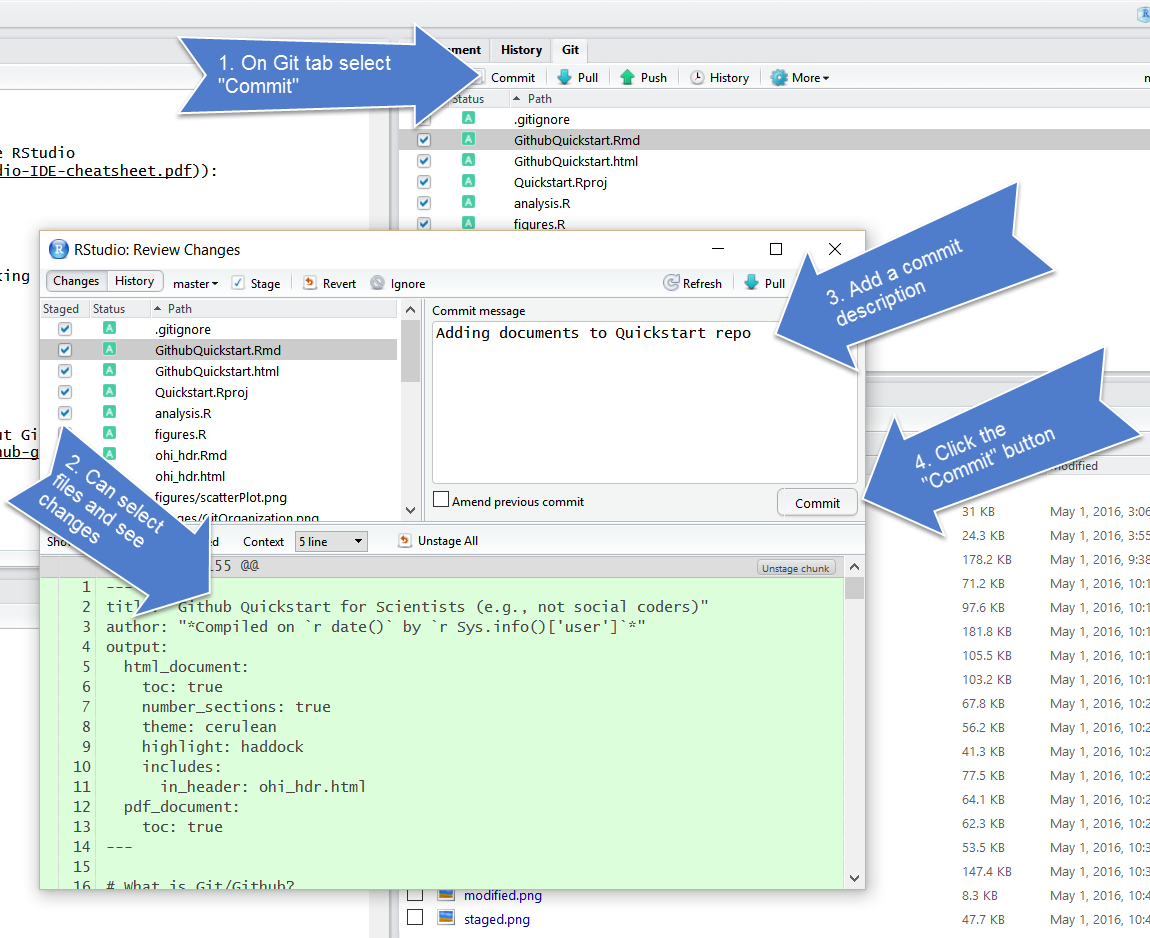
\includegraphics{img/commit.png}

\subsection{Push}\label{push}

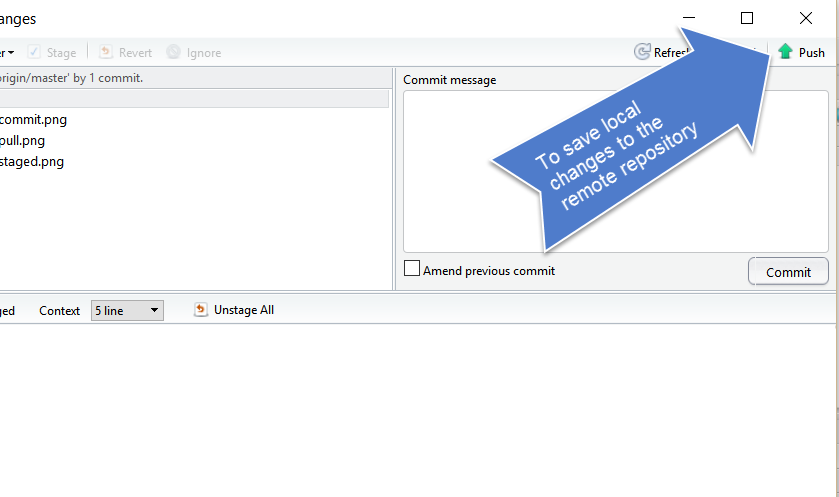
\includegraphics{img/push.png}

\section{Explore remote Github}\label{explore-remote-github}

The files you added should be on github.com:

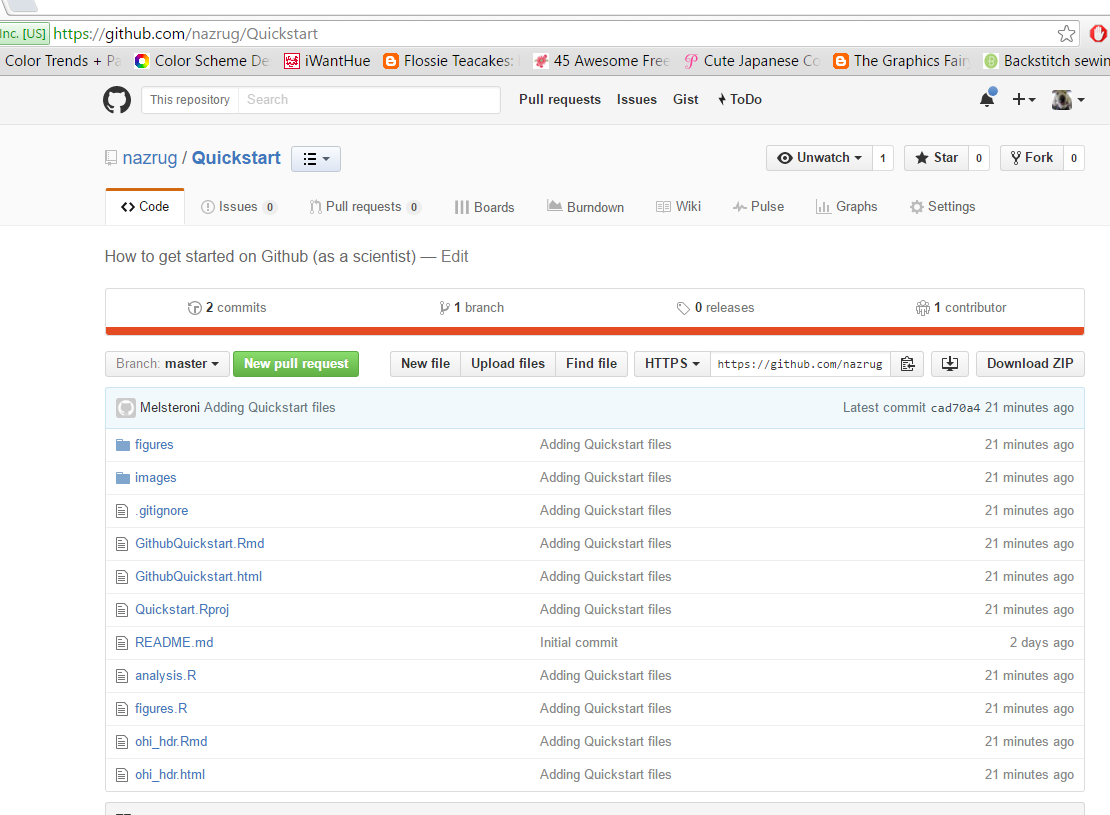
\includegraphics{img/Github_remote.png}

Let's also explore commit history, file history.

\subsection{Your turn!}\label{your-turn-3}

This time let's edit an existing file instead of adding something new.
Open your README file by clicking on it in the Files pane (lower right
corner). Write a few lines of text, save, and see what happens in your
Git Tab. Sync it to your remote repository (Github.com).

Also, go to your Finder/Windows Explorer, and copy-paste something into
your local GitHub repo. Then go back to RStudio and confirm that git
tracked it. Remember, git will track anything within that folder (the
way Dropbox does), it's not specific to RStudio!

\section{Create a new R Markdown
file}\label{create-a-new-r-markdown-file}

OK, now, let's go back to RStudio, and get ourselves back into learning
R. We are going to use R Markdown so that you can write notes to
yourself in Markdown, and have a record of all your R code. Writing R
commands in the console like we did this morning is great, but limited;
it's hard to keep track of and hard to efficiently share with others.
Plus, as your analyses get more complicated, you need to be able to see
them all in one place.

Go to File \textgreater{} New File \textgreater{} R Markdown \ldots{}
(or click the green plus in the top left corner).

Let's set up this file so we can use it for the rest of the day. I'm
going to delete all the text that is already there and write some new
text.

Here's what I'm going to write in my R Markdown file to begin:

\begin{verbatim}
---
title: "My Project"
author: "Julie"
date: "11/21/2017"
output: html_document
---

# Data wrangling with dplyr

We are going use "gapminder" data to learn `dplyr`. It's going to be amazing. 
\end{verbatim}

Now, let's save it. I'm going to call my file
\texttt{wrangle-dplyr.Rmd}.

OK. Now let's practice with some of those commands that we were working
on this morning.

Create a new chunk in your RMarkdown first in one of these ways:

\begin{itemize}
\tightlist
\item
  click ``Insert \textgreater{} R'' at the top of the editor pane
\item
  type by hand ```\{r\} ```
\item
  if you haven't deleted a chunk that came with the new file, edit that
  one
\end{itemize}

Now, let's write some R code.

\begin{verbatim}
x <- seq(1:15)
\end{verbatim}

Now, hitting return does not execute this command; remember, it's just a
text file. To execute it, we need to get what we typed in the script
down into the console. How do we do it? There are several ways (let's do
each of them):

\begin{enumerate}
\def\labelenumi{\arabic{enumi}.}
\tightlist
\item
  copy-paste this line into the console.
\item
  select the line (or simply put the cursor there), and click `Run'.
  This is available from

  \begin{enumerate}
  \def\labelenumii{\alph{enumii}.}
  \tightlist
  \item
    the bar above the script (green arrow)
  \item
    the menu bar: Code \textgreater{} Run Selected Line(s)
  \item
    keyboard shortcut: command-return
  \end{enumerate}
\item
  click the green arrow at the right of the code chunk
\end{enumerate}

\subsection{Your turn}\label{your-turn-4}

Add a few more commands to your file from this morning. Execute them by
trying the three ways above.

Then, sync your script to GitHub.

\section{Committing - how often? Tracking changes in your
files}\label{committing---how-often-tracking-changes-in-your-files}

Whenever you make changes to the files in Github, you will walk through
the Pull -\textgreater{} Stage -\textgreater{} Commit -\textgreater{}
Push steps.

I tend to do this every time I finish a task (basically when I start
getting nervous that I will lose my work). Once something is committed,
it is very difficult to lose it.

One thing that I love about about Github is that it is easy to see how
files have changed over time. Usually I compare commits through
github.com:

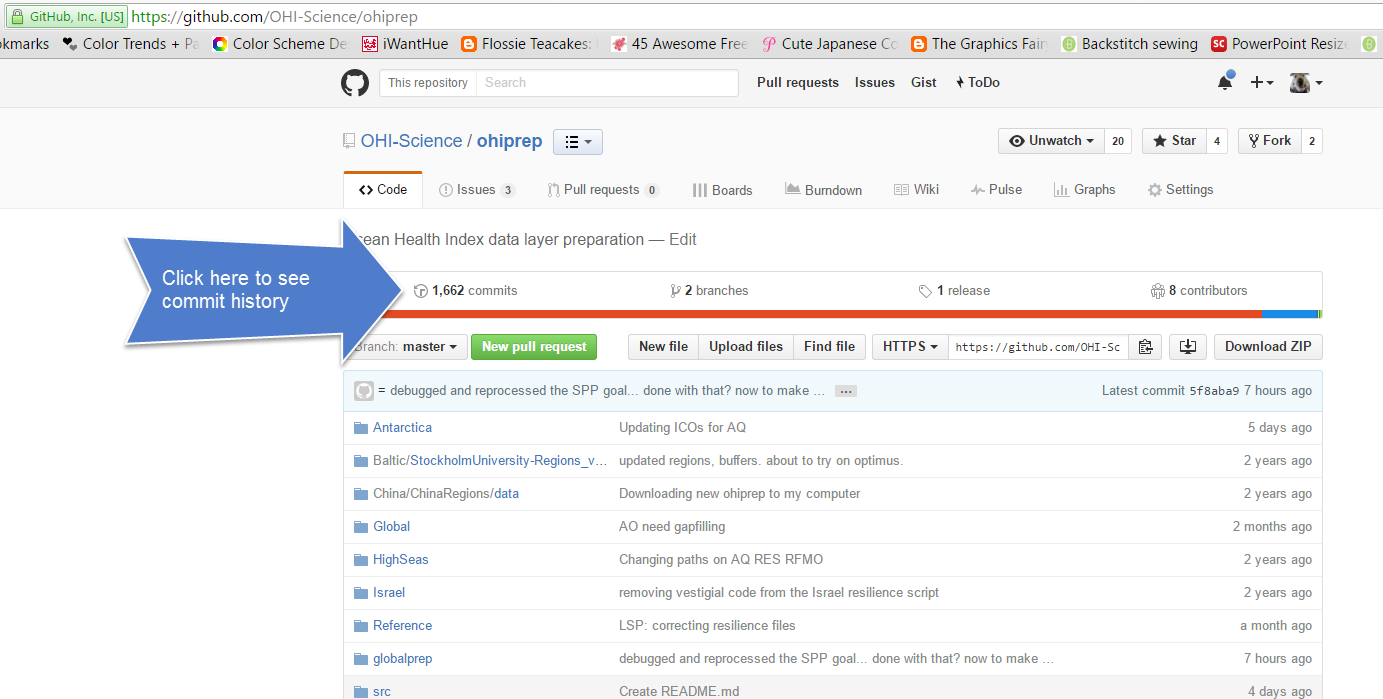
\includegraphics{img/commit_history.png}

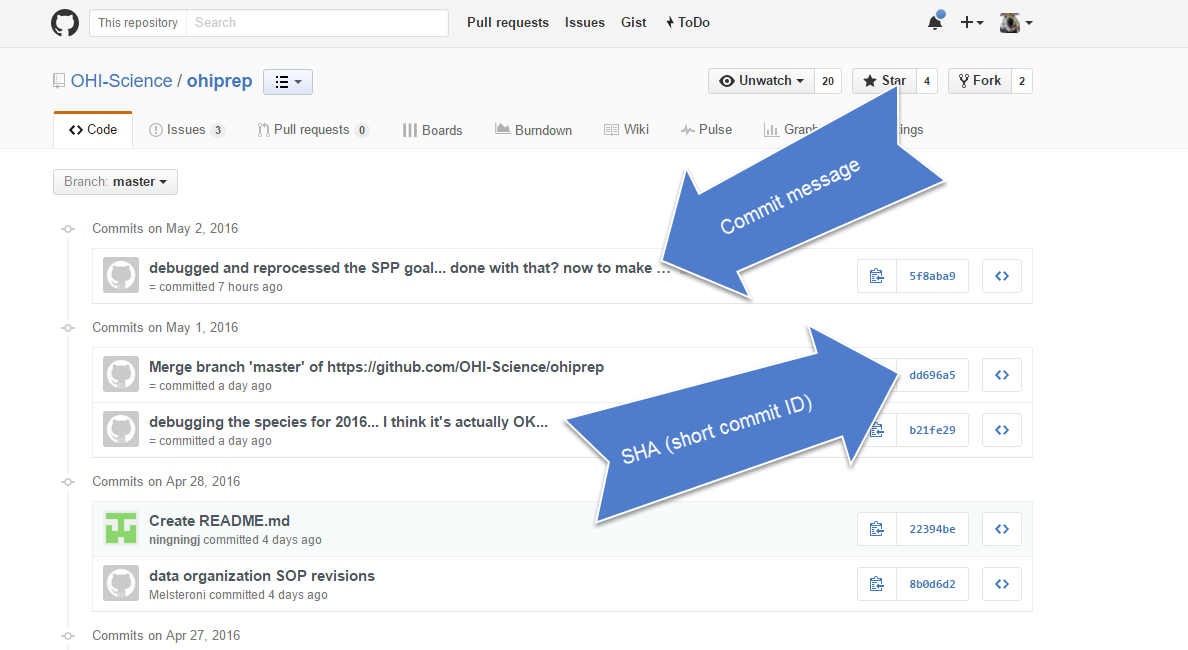
\includegraphics{img/commit_compare_2.png}

You can click on the commits to see how the files changed from the
previous commit:

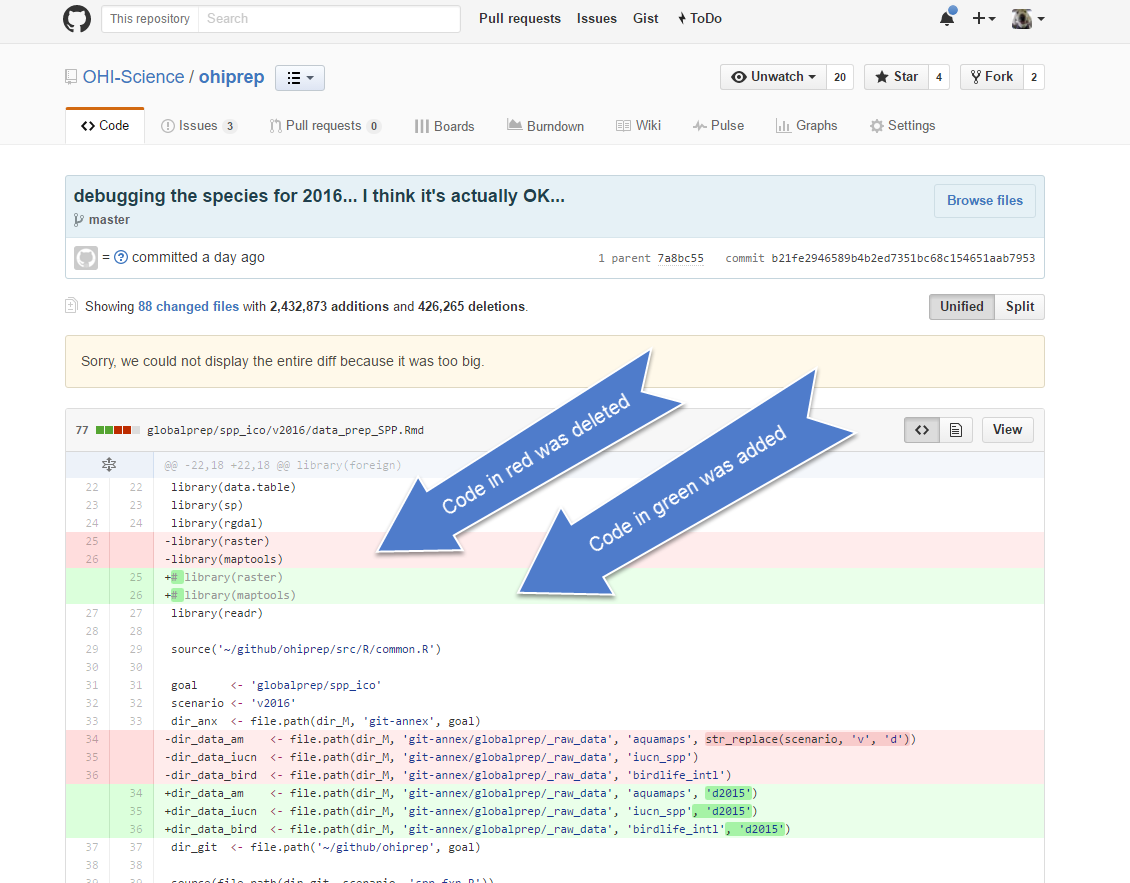
\includegraphics{img/commit_compare_3.png}

\section{Troubleshooting}\label{troubleshooting-1}

If you have problems, we'll help you out using Jenny Bryan's
\href{http://happygitwithr.com}{HappyGitWithR}, particularly the
sections on \href{http://happygitwithr.com/rstudio-see-git.html}{Detect
Git from RStudio} and
\href{http://happygitwithr.com/troubleshooting.html}{RStudio, Git,
GitHub Hell (troubleshooting)}.

You can follow along this morning with the Desktop App:
\href{https://www.youtube.com/watch?v=XdhuWDdu-rk}{3-minute youtube
video}

\chapter{Visualizing data}\label{viz}

\textbf{In development.}

\section{Objectives \& Resources}\label{objectives-resources-2}

\subsubsection{Objectives}\label{objectives-1}

\begin{itemize}
\tightlist
\item
  install our first package, \texttt{ggplot2}, by installing
  \texttt{tidyverse}
\item
  learn ggplot2 with \texttt{mpg} dataframe (important to play with
  other data than your own, you'll learn something.)
\item
  practice writing a script (maybe call it mpg\_viz.R?)
\item
  practice rstudio-github workflow
\item
  use and credit \url{http://r4ds.had.co.nz/data-visualisation.html}
\end{itemize}

Why do we start with data viz? Not only is data viz a big part of
analysis, it's a way to SEE your progress as you learn to code.
``ggplot2 implements the grammar of graphics, a coherent system for
describing and building graphs. With ggplot2, you can do more faster by
learning one system and applying it in many places.'' -
\href{http://r4ds.had.co.nz/data-visualisation.html}{R4DS}

\begin{itemize}
\item
  Conceptual and building, cheatsheet images
\item
  \url{http://r4ds.had.co.nz/data-visualisation.html}
\item
  \url{https://pdfs.semanticscholar.org/d779/6f85dabccd18673f382c100fc06f55e8b501.pdf}
\end{itemize}

\subsubsection{Resources}\label{resources-1}

Here are some resources that helped make this tutorial: -
\href{http://r4ds.had.co.nz/data-visualisation.html}{R for Data Science}
-
\href{../cheatsheets/ggplot2-cheatsheet-2.0.pdf}{ggplot2-cheatsheet-2.0.pdf}
-
\href{http://ucsb-bren.github.io/env-info/wk06_widgets.html}{Interactive
Plots and Maps - Environmental Informatics} -
\href{http://www.cookbook-r.com/Graphs/\#graphs-with-ggplot2}{Graphs
with ggplot2 - Cookbook for R} -
\href{http://www.sthda.com/english/wiki/ggplot2-essentials}{ggplot2
Essentials - STHDA}

D Robinson: - \url{http://varianceexplained.org/r/why-I-use-ggplot2/};
add screenshot of ggplot2 cheatsheet -
\url{http://varianceexplained.org/RData/}

\section{\texorpdfstring{Install our first package:
\texttt{tidyverse}}{Install our first package: tidyverse}}\label{install-our-first-package-tidyverse}

Packages are bundles of functions, along with help pages and other
goodies that make them easier for others to use, (ie. vignettes).

So far we've been using packages included in `base R'; they are
`out-of-the-box' functions. You can also install packages from online
created by the vast and growing R user community. The most traditional
place to download packages is from
\href{https://cran.r-project.org/}{CRAN, the Comprehensive R Archive
Network}. This is where you went to download R originally, and will go
again to look for updates. You can also install packages directly from
GitHub, which we'll do tomorrow.

You don't need to go to CRAN's website to install packages, we can do it
from within R with the command
\texttt{install.packages("package-name-in-quotes")}.

We are going to be using the package \texttt{ggplot2}, which is actually
bundled into a huge package called \texttt{tidyverse}. We will install
\texttt{tidyverse} now, and use a few functions from the packages
within. Also, check out
\href{https://www.tidyverse.org}{tidyverse.org/}.

\begin{Shaded}
\begin{Highlighting}[]
\NormalTok{## from CRAN:}
\KeywordTok{install.packages}\NormalTok{(}\StringTok{"tidyverse"}\NormalTok{) ## do this once only to install the package on your computer.}
\end{Highlighting}
\end{Shaded}

\begin{Shaded}
\begin{Highlighting}[]
\KeywordTok{library}\NormalTok{(tidyverse) ## do this every time you restart R and need it }
\end{Highlighting}
\end{Shaded}

When you do this, it will tell you which packages are inside of
\texttt{tidyverse} that have also been installed. Note that there are a
few name conflicts; it is alerting you that we'll be using two functions
from dplyr instead of the built-in stats package.

What's the difference between \texttt{install.packages()} and
\texttt{library()}? Why do you need both? Here's my analogy:

\begin{itemize}
\tightlist
\item
  \texttt{install.packages()} is setting up electricity for your house.
  Just need to do this once (let's ignore monthly bills).
\item
  \texttt{library()} is turning on the lights. You only turn them on
  when you need them, otherwise it wouldn't be efficient. And when you
  quit R, it turns the lights off, but the electricity lines are still
  there. So when you come back, you'll have to turn them on again with
  \texttt{library()}, but you already have your electricity set up.
\end{itemize}

You can also install packages by going to the Packages tab in the bottom
right pane. You can see the packages that you have installed (listed)
and loaded (checkbox). You can also install packages using the install
button, or check to see if any of your installed packages have updates
available (update button). You can also click on the name of the package
to see all the functions inside it --- this is a super helpful feature
that I use all the time.

\section{Aesthetic mappings}\label{aesthetic-mappings}

\begin{figure}[htbp]
\centering
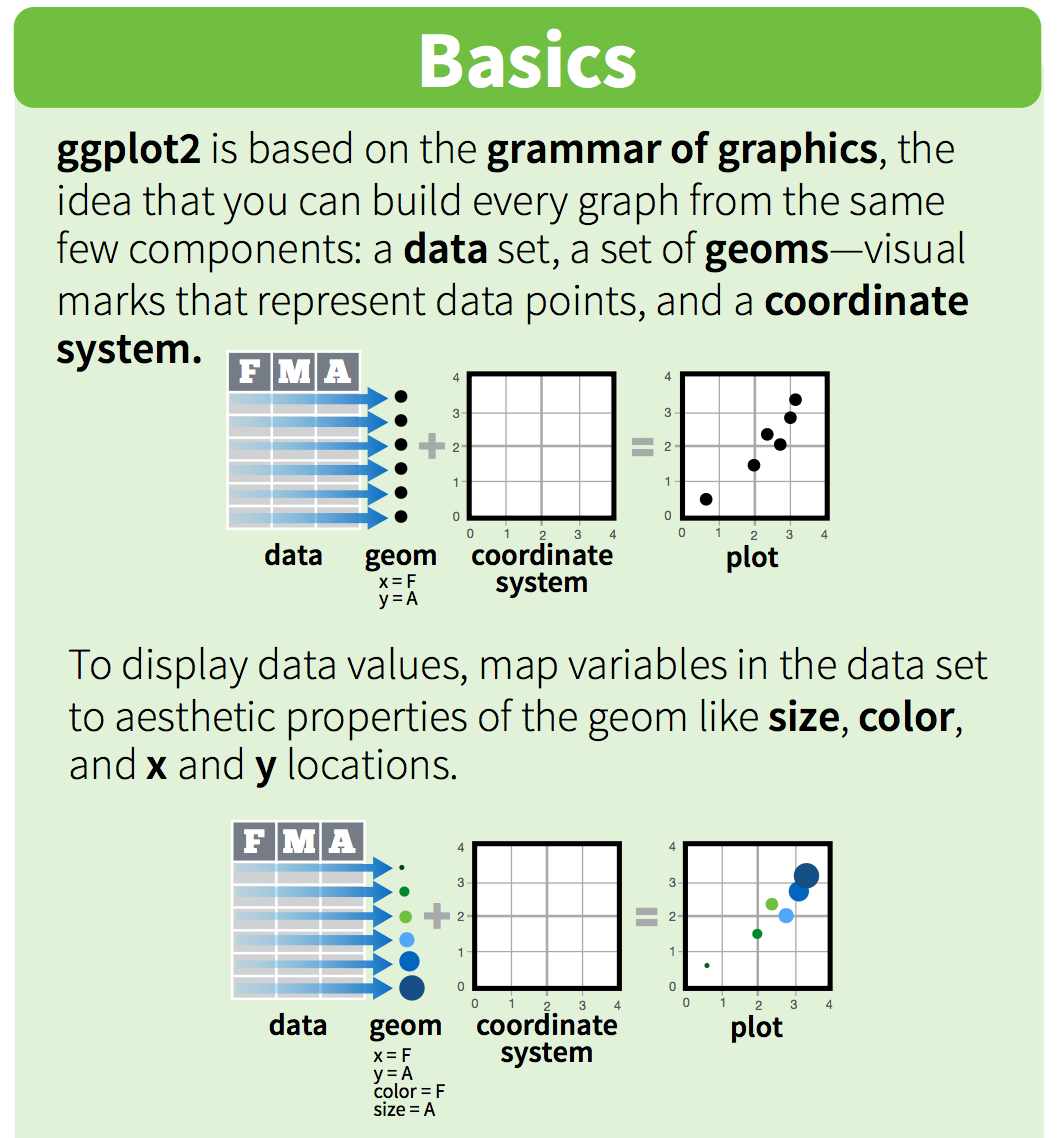
\includegraphics{img/rstudio-cheatsheet-ggplot.png}
\caption{}
\end{figure}

\section{push to GitHub}\label{push-to-github}

\subsection{Your turn}\label{your-turn-5}

\section{Common problems}\label{common-problems}

\ldots{}

\subsection{Your turn}\label{your-turn-6}

\section{The Layered Grammar of
Graphics}\label{the-layered-grammar-of-graphics}

\section{push to GitHub}\label{push-to-github-1}

Explore GitHub; show that your fig has a URL you could share with
someone

\section{end of the day: intro to Markdown
(README)?}\label{end-of-the-day-intro-to-markdown-readme}

so they can post a figure on a readme?

\section{Troubleshooting}\label{troubleshooting-2}

\chapter{Wrangling (dplyr)}\label{dplyr}

\section{\texorpdfstring{Overview of
\texttt{dplyr}}{Overview of dplyr}}\label{overview-of-dplyr}

We are going to introduce you to data wrangling in R first with the
tidyverse. The tidyverse is a new suite of packages that match a
philosophy of data science developed by Hadley Wickham and the RStudio
team. I find it to be a more straight-forward way to learn R. We will
also show you by comparison what code will look like in ``Base R'',
which means, in R without any additional packages (like the
``tidyverse'' package) installed. I like David Robinson's blog post on
the topic of
\href{http://varianceexplained.org/r/teach-hard-way}{teaching the
tidyverse first}.

For some things, base-R is more straight forward, and we'll show you
that too. Whenever we use a function that is from the tidyverse, we will
prefix it so you'll know for sure.

\textbf{Objectives}

\begin{itemize}
\tightlist
\item
  learn about tidy data
\item
  learn \texttt{dplyr} with \texttt{gapminder} data
\item
  practice RStudio-GitHub workflow
\end{itemize}

\textbf{Resources}

Today's materials are again borrowing from some excellent sources,
including:

\begin{itemize}
\tightlist
\item
  Jenny Bryan's lectures from STAT545 at UBC:
  \href{http://stat545.com/block009_dplyr-intro.html}{Introduction to
  dplyr}
\item
  Hadley Wickham and Garrett Grolemund's \href{http://r4ds.had.co.nz/}{R
  for Data Science}
\item
  Software Carpentry's R for reproducible scientific analysis materials:
  \href{http://swcarpentry.github.io/r-novice-gapminder/13-dplyr.html}{Dataframe
  manipulation with dplyr}
\item
  First developed for
  \href{http://remi-daigle.github.io/2016-04-15-UCSB/dplyr/}{Software
  Carpentry at UCSB}
\item
  \href{http://www.rstudio.com/wp-content/uploads/2015/02/data-wrangling-cheatsheet.pdf}{RStudio's
  data wrangling cheatsheet}
\item
  \href{https://www.rstudio.com/resources/webinars/data-wrangling-with-r-and-rstudio/}{RStudio's
  data wrangling webinar}
\end{itemize}

\section{Prerequisites}\label{prerequisites-1}

\textbf{R Skill Level}: Beginner - you've got basics of R down and are
ready to wrangle your data.

We will use the \texttt{dplyr} package, which will have been installed
with:

\begin{Shaded}
\begin{Highlighting}[]
\KeywordTok{install.packages}\NormalTok{(}\StringTok{'tidyverse'}\NormalTok{)}
\end{Highlighting}
\end{Shaded}

\section{Tidy Data}\label{tidy-data}

Hadley Wickham, RStudio's Chief Scientist, has been building R packages
for data wrangling and visualization based on the idea of \textbf{tidy
data}.

Tidy data has a simple convention: put variables in the columns and
observations in the rows.

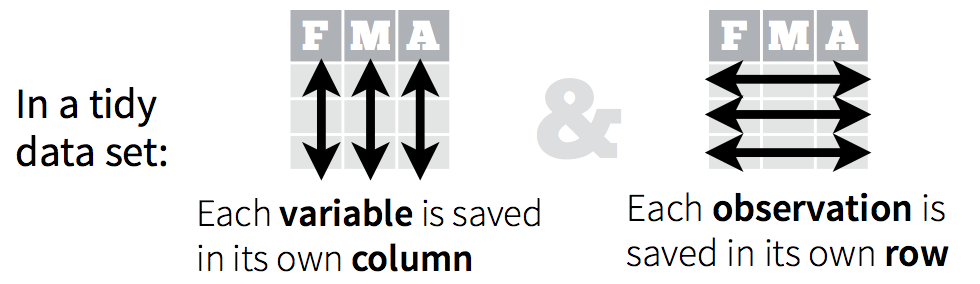
\includegraphics{img/tidy_data.png} The \texttt{mpg} dataset we were
working with this morning was an example of tidy data. When data are
tidy, you are set up to work with it for your analyses, plots, etc.
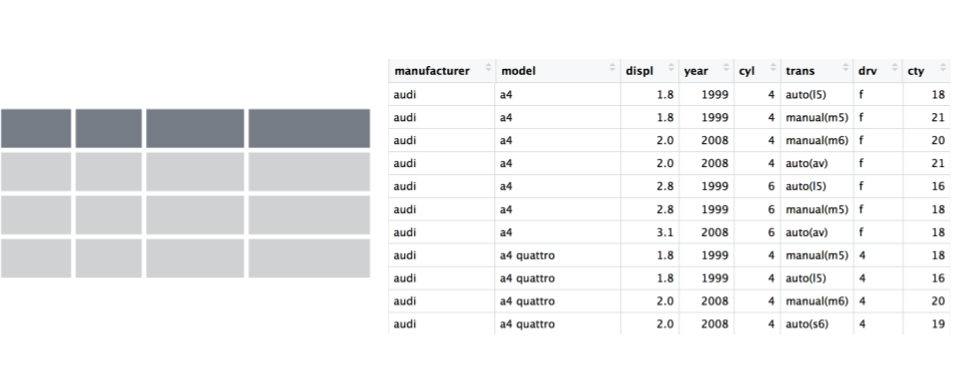
\includegraphics{img/tidy_img_mpg.png}

Right now we are going to use \texttt{dplyr} to wrangle this tidyish
data set (the transform part of the cycle), and then come back to
tidying messy data using \texttt{tidyr} once we've had some fun
wrangling. These are both part of the \texttt{tidyverse} package that
we've already installed:

\begin{figure}[htbp]
\centering
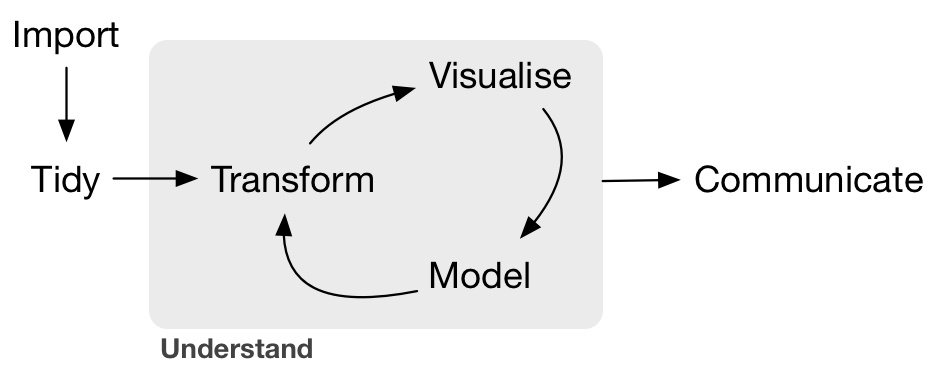
\includegraphics{img/r4ds_data-science.png}
\caption{}
\end{figure}

And actually, Hadley Wickham and RStudio have created a ton of packages
that help you at every step of the way here. This is from one of
Hadley's recent presentations:

\begin{figure}[htbp]
\centering
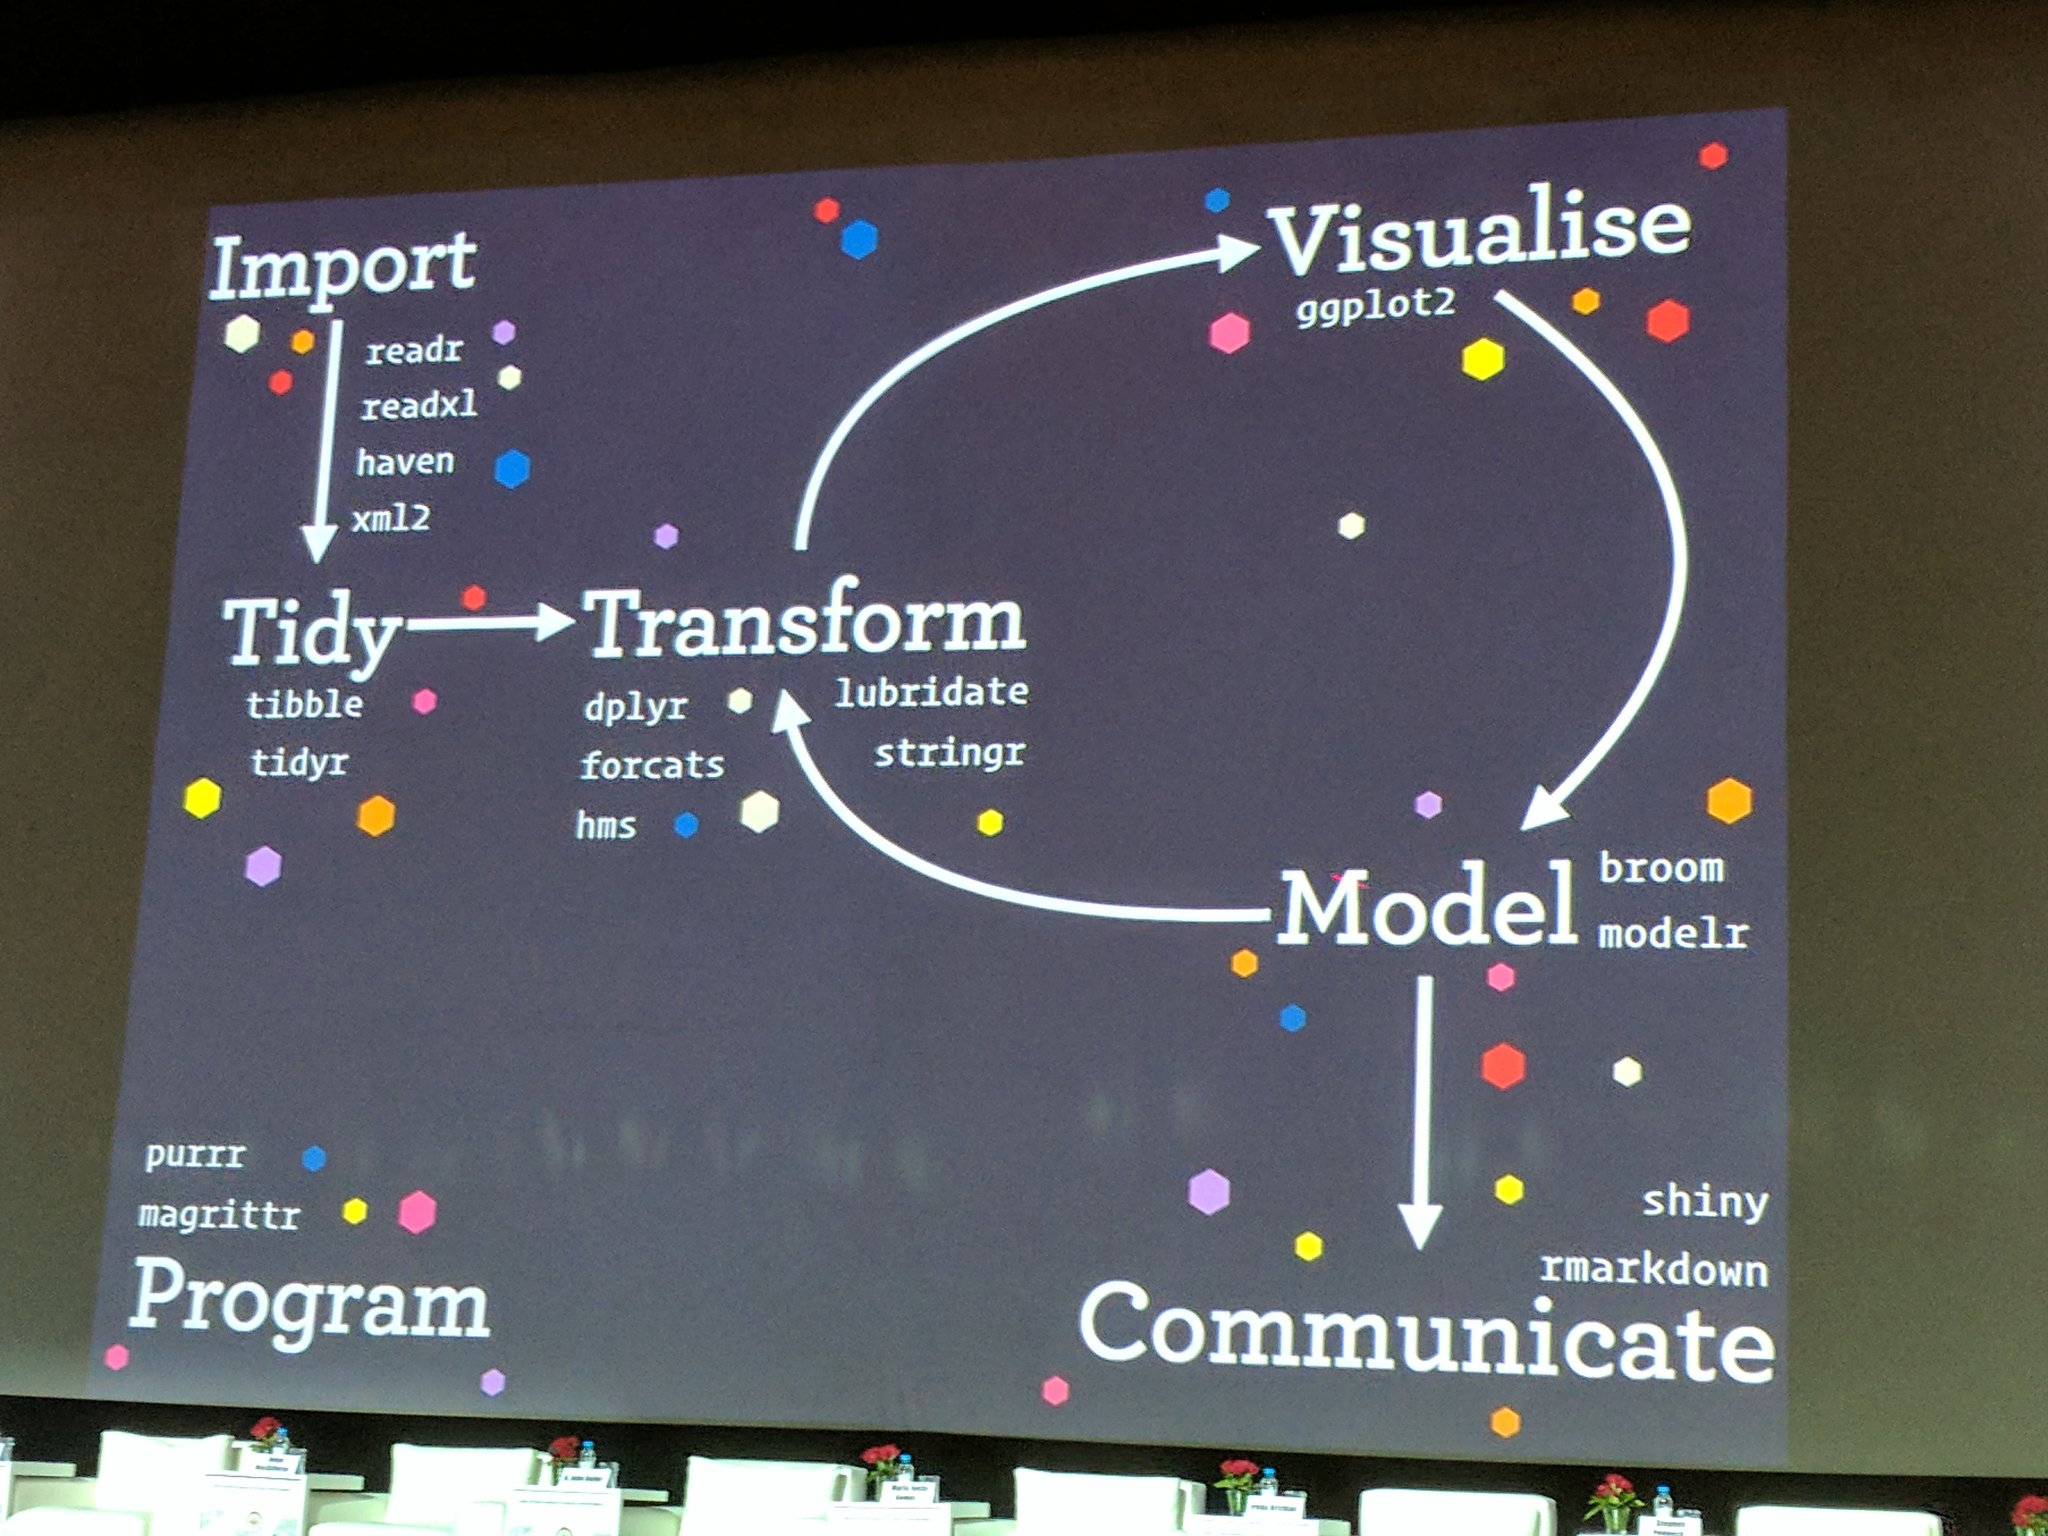
\includegraphics{img/tidyverse_wickham_pres.jpg}
\caption{}
\end{figure}

\subsection{setup}\label{setup}

We'll do this in a new RMarkdown file.

\textbf{Here's what to do:}

\begin{enumerate}
\def\labelenumi{\arabic{enumi}.}
\tightlist
\item
  Clear your workspace (Session \textgreater{} Restart R)
\item
  New File \textgreater{} R Markdown\ldots{}
\item
  Save as \texttt{gapminder-wrangle.Rmd}
\item
  Delete the irrelevant text and write a little note to yourself about
  how we'll be warngling gapminder data using dplyr. You can edit the
  title too if you need to.
\end{enumerate}

\section{Explore the gapminder
data.frame}\label{explore-the-gapminder-data.frame}

We will work with some of the data from the
\href{http://www.gapminder.org}{Gapminder project}.

The data are on GitHub, in our course webite. Navigate there by going
to:

github.com \textgreater{} ohi-science \textgreater{}
data-science-training \textgreater{} data \textgreater{} gapminder.csv

or by copy-pasting this in the browser:
\texttt{https://github.com/OHI-Science/data-science-training/blob/master/data/gapminder.csv}

Have a look at the data. It's a .csv file, which you've probably
encountered before, but GitHub has formatted it nicely so it's easy to
look at. You can see that for every country and year, there are several
columns with data in them.

\begin{figure}[htbp]
\centering
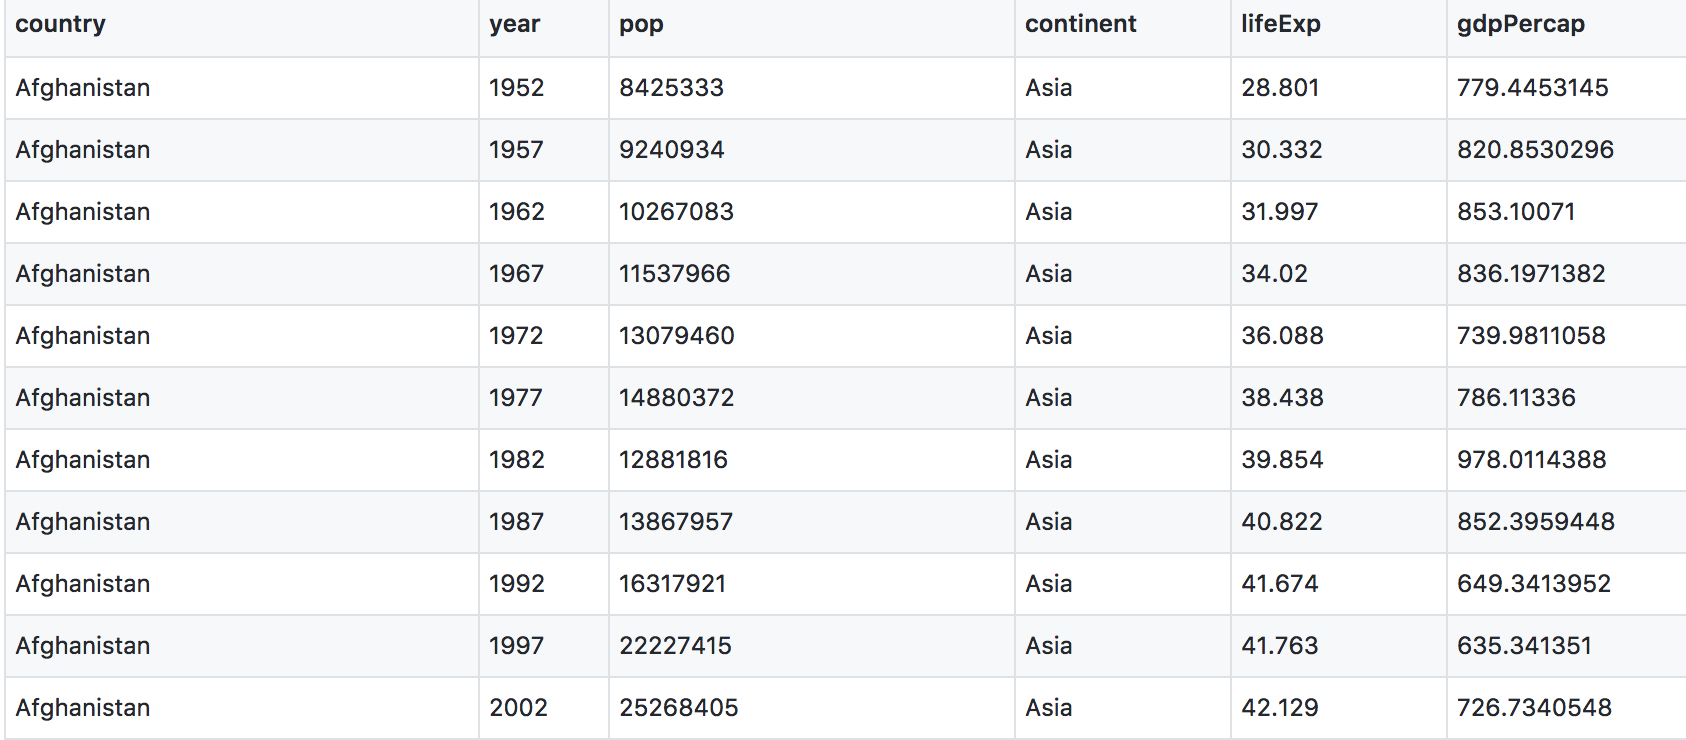
\includegraphics{img/gapminder_gh.png}
\caption{}
\end{figure}

\subsection{\texorpdfstring{read data with
\texttt{readr::read\_csv()}}{read data with readr::read\_csv()}}\label{read-data-with-readrread_csv}

We can read this data into R directly from GitHub, without downloading
it. We can do that by clicking on the Raw button on the top-right of the
data. This displays it as the raw csv file, without formatting. Copy the
url:

\url{https://raw.githubusercontent.com/jules32/2017-11-30-MBARI/gh-pages/data/gapminder.csv}

Now, let's go back to RStudio. In our R Markdown, let's read this csv
file and name the variable ``gapminder''. We will use the read\_csv
function from the readr package (part of the tidyverse, so it's already
installed!). And for comparison, you could also do it in base-R.

\begin{Shaded}
\begin{Highlighting}[]
\NormalTok{## read gapminder csv. Note the readr:: prefix identifies which package it's in}
\NormalTok{gapminder <-}\StringTok{ }\NormalTok{readr::}\KeywordTok{read_csv}\NormalTok{(}\StringTok{'https://raw.githubusercontent.com/jules32/2017-11-30-MBARI/gh-pages/data/gapminder.csv'}\NormalTok{) }
\end{Highlighting}
\end{Shaded}

Let's inspect:

\begin{Shaded}
\begin{Highlighting}[]
\NormalTok{## explore the gapminder dataset}
\NormalTok{gapminder }\CommentTok{# this is super long! Let's inspect in different ways}
\end{Highlighting}
\end{Shaded}

Let's use \texttt{head} and \texttt{tail}:

\begin{Shaded}
\begin{Highlighting}[]
\KeywordTok{head}\NormalTok{(gapminder) }\CommentTok{# shows first 6}
\KeywordTok{tail}\NormalTok{(gapminder) }\CommentTok{# shows last 6}

\KeywordTok{head}\NormalTok{(gapminder, }\DecValTok{10}\NormalTok{) }\CommentTok{# shows first X that you indicate}
\KeywordTok{tail}\NormalTok{(gapminder, }\DecValTok{12}\NormalTok{) }\CommentTok{# guess what this does!}
\end{Highlighting}
\end{Shaded}

\texttt{str()} will provide a sensible description of almost anything:
when in doubt, just \texttt{str()} some of the recently created objects
to get some ideas about what to do next.

\begin{Shaded}
\begin{Highlighting}[]
\KeywordTok{str}\NormalTok{(gapminder) }\CommentTok{# ?str - displays the structure of an object}
\end{Highlighting}
\end{Shaded}

\texttt{gapminder} is a \texttt{data.frame}. We aren't going to get into
the other types of data receptacles today (`arrays', `matrices'),
because working with data.frames is what you should primarily use. Why?

\begin{itemize}
\tightlist
\item
  data.frames package related variables neatly together, great for
  analysis
\item
  most functions, including the latest and greatest packages actually
  \textbf{require} that your data be in a data.frame
\item
  data.frames can hold variables of different flavors such as

  \begin{itemize}
  \tightlist
  \item
    character data (country or continent names; ``Characters (chr)'')
  \item
    quantitative data (years, population; ``Integers (int)'' or
    ``Numeric (num)'')
  \item
    categorical information (male vs.~female)
  \end{itemize}
\end{itemize}

We can also see the \texttt{gapminder} variable in RStudio's Environment
pane (top right)

More ways to learn basic info on a data.frame.

\begin{Shaded}
\begin{Highlighting}[]
\KeywordTok{names}\NormalTok{(gapminder)}
\KeywordTok{dim}\NormalTok{(gapminder)    }\CommentTok{# ?dim dimension}
\KeywordTok{ncol}\NormalTok{(gapminder)   }\CommentTok{# ?ncol number of columns}
\KeywordTok{nrow}\NormalTok{(gapminder)   }\CommentTok{# ?nrow number of rows}
\end{Highlighting}
\end{Shaded}

We can combine using \texttt{c()} to reverse-engineer \texttt{dim()}!
Just a side-note here, but I wanted to introduce you to \texttt{c()}:
we'll use it later.

\begin{Shaded}
\begin{Highlighting}[]
\KeywordTok{c}\NormalTok{(}\KeywordTok{nrow}\NormalTok{(gapminder), }\KeywordTok{ncol}\NormalTok{(gapminder)) }\CommentTok{# ?c combines values into a vector or list. }
\end{Highlighting}
\end{Shaded}

A statistical overview can be obtained with \texttt{summary()}

\begin{Shaded}
\begin{Highlighting}[]
\KeywordTok{summary}\NormalTok{(gapminder)}
\end{Highlighting}
\end{Shaded}

\subsection{Look at the variables inside a
data.frame}\label{look-at-the-variables-inside-a-data.frame}

To specify a single variable from a data.frame, use the dollar sign
\texttt{\$}. The \texttt{\$} operator is a way to extract of replace
parts of an object--check out the help menu for \texttt{\$}. It's a
common operator you'll see in R.

\begin{Shaded}
\begin{Highlighting}[]
\NormalTok{gapminder$lifeExp }\CommentTok{# very long! hard to make sense of...}
\KeywordTok{head}\NormalTok{(gapminder$lifeExp) }\CommentTok{# can do the same tests we tried before}
\KeywordTok{str}\NormalTok{(gapminder$lifeExp) }\CommentTok{# it is a single numeric vector}
\KeywordTok{summary}\NormalTok{(gapminder$lifeExp) }\CommentTok{# same information, just formatted slightly differently}
\end{Highlighting}
\end{Shaded}

\section{\texorpdfstring{\texttt{dplyr}
overview}{dplyr overview}}\label{dplyr-overview}

OK, so let's start wrangling with dplyr.

There are five \texttt{dplyr} functions that you will use to do the vast
majority of data manipulations:

\begin{itemize}
\tightlist
\item
  \textbf{\texttt{filter()}}: pick observations by their values
\end{itemize}

\begin{itemize}
\tightlist
\item
  \textbf{\texttt{select()}}: pick variables by their names
\end{itemize}

\begin{itemize}
\tightlist
\item
  \textbf{\texttt{mutate()}}: create new variables with functions of
  existing variables
\end{itemize}

\begin{itemize}
\tightlist
\item
  \textbf{\texttt{summarise()}}: collapse many values down to a single
  summary
\end{itemize}

\begin{itemize}
\tightlist
\item
  \textbf{\texttt{arrange()}}: reorder the rows
\end{itemize}

These can all be used in conjunction with \texttt{group\_by()} which
changes the scope of each function from operating on the entire dataset
to operating on it group-by-group. These six functions provide the verbs
for a language of data manipulation.

All verbs work similarly:

\begin{enumerate}
\def\labelenumi{\arabic{enumi}.}
\tightlist
\item
  The first argument is a data frame.
\item
  The subsequent arguments describe what to do with the data frame. You
  can refer to columns in the data frame directly without using
  \texttt{\$}.
\item
  The result is a new data frame.
\end{enumerate}

Together these properties make it easy to chain together multiple simple
steps to achieve a complex result.

\subsection{\texorpdfstring{install \texttt{tidyverse} (which has
\texttt{dplyr}
inside)}{install tidyverse (which has dplyr inside)}}\label{install-tidyverse-which-has-dplyr-inside}

In your R Markdow file, let's make sure we've got our libraries loaded.
Write the following:

\begin{Shaded}
\begin{Highlighting}[]
\KeywordTok{library}\NormalTok{(tidyverse)     ## install.packages("tidyverse")}
\end{Highlighting}
\end{Shaded}

This is becoming standard practice for how to load a library in a file,
and if you get an error that the library doesn't exist, you can install
the package easily by running the code within the comment (highlight
\texttt{install.packages("tidyverse")} and run it).

\section{\texorpdfstring{Use \texttt{dplyr::filter()} to subset data
row-wise
(observations).}{Use dplyr::filter() to subset data row-wise (observations).}}\label{use-dplyrfilter-to-subset-data-row-wise-observations.}

You will want to isolate bits of your data; maybe you want to just look
at a single country or a few years. R calls this subsetting.

\texttt{filter()} is a function in \texttt{dplyr} that takes logical
expressions and returns the rows for which all are \texttt{TRUE}.

Visually, we are doing this (thanks RStudio for your
\href{http://www.rstudio.com/wp-content/uploads/2015/02/data-wrangling-cheatsheet.pdf}{cheatsheet}):

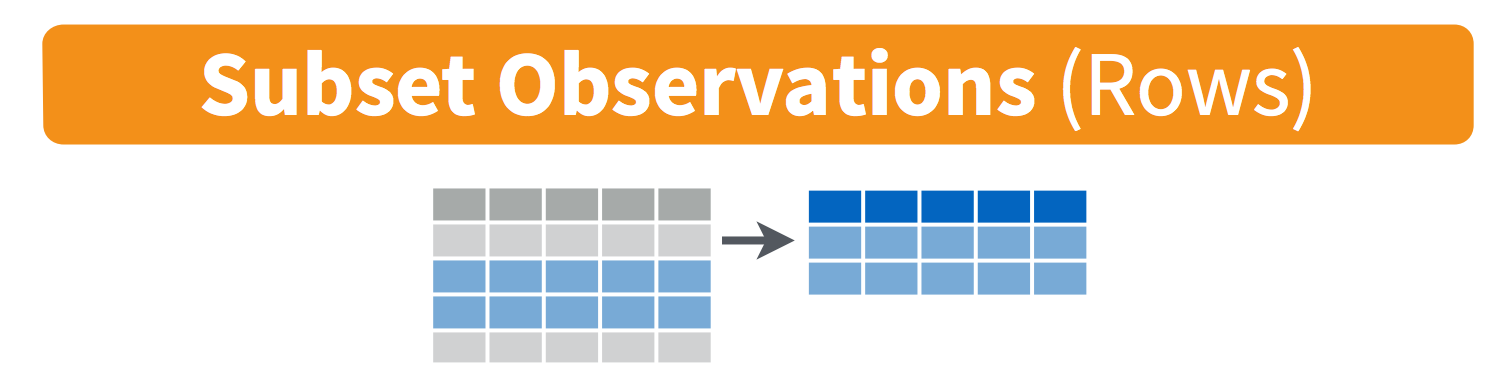
\includegraphics{img/rstudio-cheatsheet-filter.png} Remember your
logical expressions from this morning? We'll use \texttt{\textless{}}
and \texttt{==} here.

\begin{Shaded}
\begin{Highlighting}[]
\KeywordTok{filter}\NormalTok{(gapminder, lifeExp <}\StringTok{ }\DecValTok{29}\NormalTok{)}
\end{Highlighting}
\end{Shaded}

You can say this out loud: ``Filter the gapminder data for life
expectancy less than 29''. Notice that when we do this, all the columns
are returned, but just the rows that have the life expectancy less than
29. We've subsetted by row.

Let's try another: ``Filter the gapminder data for the country Mexico''.

\begin{Shaded}
\begin{Highlighting}[]
\KeywordTok{filter}\NormalTok{(gapminder, country ==}\StringTok{ "Mexico"}\NormalTok{)}
\end{Highlighting}
\end{Shaded}

How about if we want two country names? We can't use the \texttt{==}
operator here, because it can only operate on one thing at a time. We
will use the \texttt{\%in\%} operator:

\begin{Shaded}
\begin{Highlighting}[]
\KeywordTok{filter}\NormalTok{(gapminder, country %in%}\StringTok{ }\KeywordTok{c}\NormalTok{(}\StringTok{"Mexico"}\NormalTok{, }\StringTok{"Peru"}\NormalTok{))}
\end{Highlighting}
\end{Shaded}

How about if we want Mexico in 2002? You can pass filter different
criteria:

\begin{Shaded}
\begin{Highlighting}[]
\KeywordTok{filter}\NormalTok{(gapminder, country ==}\StringTok{ "Mexico"}\NormalTok{, year ==}\StringTok{ }\DecValTok{2002}\NormalTok{)}
\end{Highlighting}
\end{Shaded}

\section{Your turn}\label{your-turn-7}

What is the mean life expenctancy of Sweden? Hint: do this in 2 steps by
assigning a variable and then using the \texttt{mean()} function.

Then, sync to Github.com (pull, stage, commit, push).

\subsection{Answer}\label{answer}

\begin{Shaded}
\begin{Highlighting}[]
\NormalTok{x <-}\StringTok{ }\KeywordTok{filter}\NormalTok{(gapminder, country ==}\StringTok{ "Sweden"}\NormalTok{)  }
\KeywordTok{mean}\NormalTok{(x$lifeExp)  }
\end{Highlighting}
\end{Shaded}

\section{Meet the new pipe operator}\label{meet-the-new-pipe-operator}

Before we go any further, we should exploit the new pipe operator that
\texttt{dplyr} imports from the
\href{https://github.com/smbache/magrittr}{\texttt{magrittr}} package by
Stefan Bache. \textbf{This is going to change your data analytical
life}. You no longer need to enact multi-operation commands by nesting
them inside each other. And we won't need to make temporary variables
like we did in the Sweden example above. This new syntax leads to code
that is much easier to write and to read: it actually tells the story of
your analysis.

Here's what it looks like: \texttt{\%\textgreater{}\%}. The RStudio
keyboard shortcut: Ctrl + Shift + M (Windows), Cmd + Shift + M (Mac).

Let's demo then I'll explain:

\begin{Shaded}
\begin{Highlighting}[]
\NormalTok{gapminder %>%}\StringTok{ }\KeywordTok{head}\NormalTok{()}
\end{Highlighting}
\end{Shaded}

This is equivalent to \texttt{head(gapminder)}. This pipe operator takes
the thing on the left-hand-side and \textbf{pipes} it into the function
call on the right-hand-side -- literally, drops it in as the first
argument.

Never fear, you can still specify other arguments to this function! To
see the first 3 rows of Gapminder, we could say
\texttt{head(gapminder,\ 3)} or this:

\begin{Shaded}
\begin{Highlighting}[]
\NormalTok{gapminder %>%}\StringTok{ }\KeywordTok{head}\NormalTok{(}\DecValTok{3}\NormalTok{)}
\end{Highlighting}
\end{Shaded}

\textbf{I've advised you to think ``gets'' whenever you see the
assignment operator, \texttt{\textless{}-}. Similary, you should think
``and then'' whenever you see the pipe operator,
\texttt{\%\textgreater{}\%}.}

You are probably not impressed yet, but the magic will soon happen.

Fun break: check out
\href{https://twitter.com/backerman150/status/926479565869993984}{this
gif about \%\textgreater{}\% from Twitter}.

\section{\texorpdfstring{Use \texttt{dplyr::select()} to subset data
column-wise
(variables)}{Use dplyr::select() to subset data column-wise (variables)}}\label{use-dplyrselect-to-subset-data-column-wise-variables}

Back to \texttt{dplyr} \ldots{}

Use \texttt{select()} to subset the data on variables or columns.

Visually, we are doing this (thanks RStudio for your
\href{http://www.rstudio.com/wp-content/uploads/2015/02/data-wrangling-cheatsheet.pdf}{cheatsheet}):

\begin{figure}[htbp]
\centering
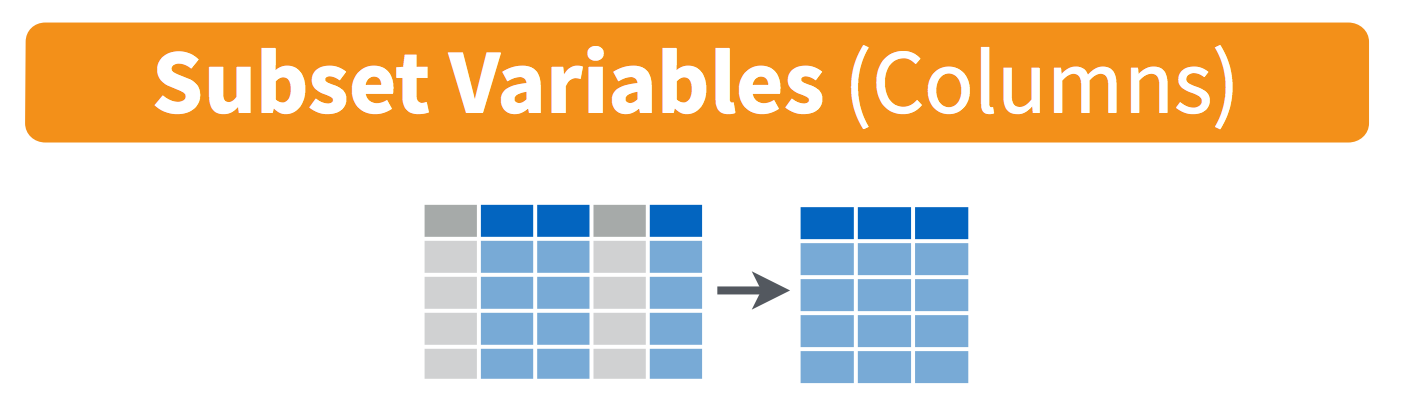
\includegraphics{img/rstudio-cheatsheet-select.png}
\caption{}
\end{figure}

Here's a conventional call. Again, see that we can select multiple
columns just with a comma, after we specify the data frame (gapminder).

\begin{Shaded}
\begin{Highlighting}[]
\KeywordTok{select}\NormalTok{(gapminder, year, lifeExp) }
\end{Highlighting}
\end{Shaded}

But using what we just learned, with a pipe, we can do this:

\begin{Shaded}
\begin{Highlighting}[]
\NormalTok{gapminder %>%}\StringTok{ }\KeywordTok{select}\NormalTok{(year, lifeExp)}
\end{Highlighting}
\end{Shaded}

Let's write it again but using multiple lines so it's nicer to read. And
let's add a second pipe operator to pipe through \texttt{head}:

\begin{Shaded}
\begin{Highlighting}[]
\NormalTok{gapminder %>%}
\StringTok{  }\KeywordTok{select}\NormalTok{(year, lifeExp) %>%}
\StringTok{  }\KeywordTok{head}\NormalTok{(}\DecValTok{4}\NormalTok{)}
\end{Highlighting}
\end{Shaded}

Think: ``Take \texttt{gapminder}, then select the variables year and
lifeExp, then show the first 4 rows.''

Being able to read a story out of code like this is really
game-changing.

\subsection{Revel in the convenience}\label{revel-in-the-convenience}

Let's take the gapminder data and filter for the country Cambodia, and
select 4 of the columns: country, year, pop, gdpPercap.

\begin{Shaded}
\begin{Highlighting}[]
\NormalTok{gapminder %>%}
\StringTok{  }\KeywordTok{filter}\NormalTok{(country ==}\StringTok{ "Cambodia"}\NormalTok{) %>%}
\StringTok{  }\KeywordTok{select}\NormalTok{(country, year, pop, gdpPercap) }
\end{Highlighting}
\end{Shaded}

But entering each column by hand can be tedious, especially since there
are fewer columns we \emph{don't} want. So instead, we can do:

\begin{Shaded}
\begin{Highlighting}[]
\NormalTok{gapminder %>%}
\StringTok{  }\KeywordTok{filter}\NormalTok{(country ==}\StringTok{ "Cambodia"}\NormalTok{) %>%}
\StringTok{  }\KeywordTok{select}\NormalTok{(-continent, -lifeExp) }\CommentTok{# you can use - to deselect columns}
\end{Highlighting}
\end{Shaded}

\section{\texorpdfstring{Use \texttt{dplyr::mutate()} to add new
variables}{Use dplyr::mutate() to add new variables}}\label{use-dplyrmutate-to-add-new-variables}

Alright, let's keep going.

Let's say we needed to add an index column so we know which order these
data came in. Let's not make a new variable, let's add a column to our
gapminder data frame. How do we do that? With the \texttt{mutate()}
function.

Visually, we are doing this (thanks RStudio for your
\href{http://www.rstudio.com/wp-content/uploads/2015/02/data-wrangling-cheatsheet.pdf}{cheatsheet}):

\begin{figure}[htbp]
\centering
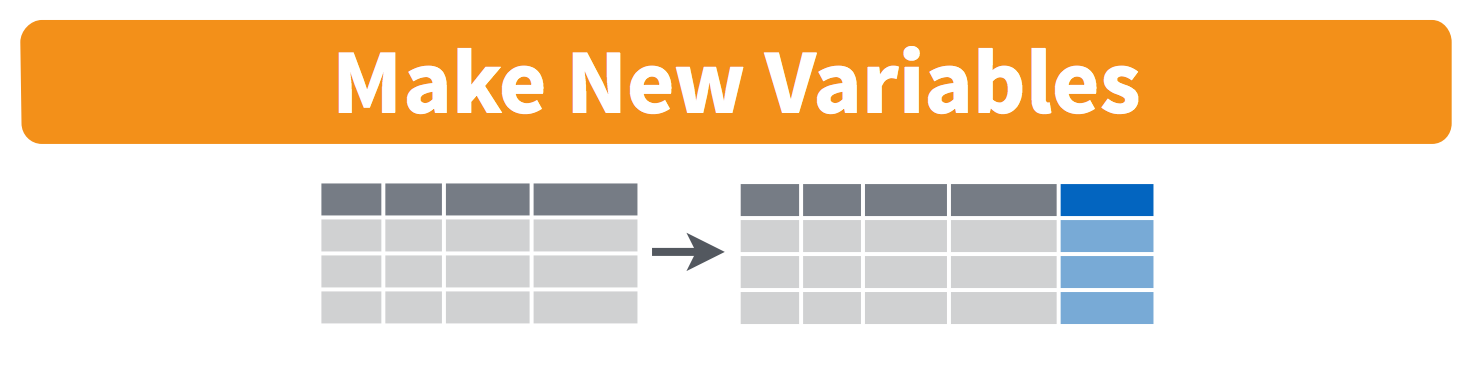
\includegraphics{img/rstudio-cheatsheet-mutate.png}
\caption{}
\end{figure}

We will name our new column index. We will name the new column `index';
and we assign it with a single \texttt{=}. Notice that we can use the
\texttt{nrow} function \emph{within} our mutate call:

\begin{Shaded}
\begin{Highlighting}[]
\NormalTok{gapminder %>%}\StringTok{ }
\StringTok{  }\KeywordTok{mutate}\NormalTok{(}\DataTypeTok{index =} \DecValTok{1}\NormalTok{:}\KeywordTok{nrow}\NormalTok{(gapminder))}
\end{Highlighting}
\end{Shaded}

OK, let's do another example. Imagine we wanted to recover each
country's GDP. After all, the Gapminder data has a variable for
population and GDP per capita.

\begin{Shaded}
\begin{Highlighting}[]
\NormalTok{gapminder %>%}
\StringTok{  }\KeywordTok{mutate}\NormalTok{(}\DataTypeTok{gdp =} \NormalTok{pop *}\StringTok{ }\NormalTok{gdpPercap)}
\end{Highlighting}
\end{Shaded}

\section{Your turn}\label{your-turn-8}

Find the maximum gdpPercap of Egypt and Vietnam Create a new column.

Then, sync to Github.com (pull, stage, commit, push).

\subsection{Answer}\label{answer-1}

\begin{Shaded}
\begin{Highlighting}[]
\NormalTok{gapminder %>%}
\StringTok{  }\KeywordTok{select}\NormalTok{(-continent, -lifeExp) %>%}\StringTok{ }\CommentTok{# not super necessary but to simplify}
\StringTok{  }\KeywordTok{filter}\NormalTok{(country ==}\StringTok{ "Egypt"}\NormalTok{) %>%}
\StringTok{  }\KeywordTok{mutate}\NormalTok{(}\DataTypeTok{gdp =} \NormalTok{pop *}\StringTok{ }\NormalTok{gdpPercap) %>%}
\StringTok{  }\KeywordTok{mutate}\NormalTok{(}\DataTypeTok{max_gdp =} \KeywordTok{max}\NormalTok{(gdp))}

\NormalTok{## you can also create multiple variables within the same mutate(), and line them up so they are easier to read:}
\NormalTok{gapminder %>%}
\StringTok{  }\KeywordTok{select}\NormalTok{(-continent, -lifeExp) %>%}\StringTok{ }\CommentTok{# not super necessary but to simplify}
\StringTok{  }\KeywordTok{filter}\NormalTok{(country ==}\StringTok{ "Vietnam"}\NormalTok{) %>%}\StringTok{ }
\StringTok{  }\KeywordTok{mutate}\NormalTok{(}\DataTypeTok{gdp     =} \NormalTok{pop *}\StringTok{ }\NormalTok{gdpPercap,}
         \DataTypeTok{max_gdp =} \KeywordTok{max}\NormalTok{(gdp))}
\end{Highlighting}
\end{Shaded}

With the things we know so far, the answers you have are maybe a bit
limiting. First, We had to act on Egypt and Vietnam separately, and
repeat the same code. Copy-pasting like this is also super error prone.

And second, this \texttt{max\_gdpPercap} column is pretty redundant,
because it's a repeated value a ton of times. Sometimes this is exactly
what you want! You are now set up nicely to maybe take a proportion of
gdpPercap/max\_gdpPercap for each year or something. But maybe you just
wanted that max\_gdpPercap for something else. Let's keep going\ldots{}

\section{\texorpdfstring{\texttt{dplyr::group\_by()} to operate on
groups}{dplyr::group\_by() to operate on groups}}\label{dplyrgroup_by-to-operate-on-groups}

Let's tackle that first issue first. So how do we less painfully
calculate the max gdpPercap for all countries?

Visually, we are doing this (thanks RStudio for your
\href{http://www.rstudio.com/wp-content/uploads/2015/02/data-wrangling-cheatsheet.pdf}{cheatsheet}):

\begin{figure}[htbp]
\centering
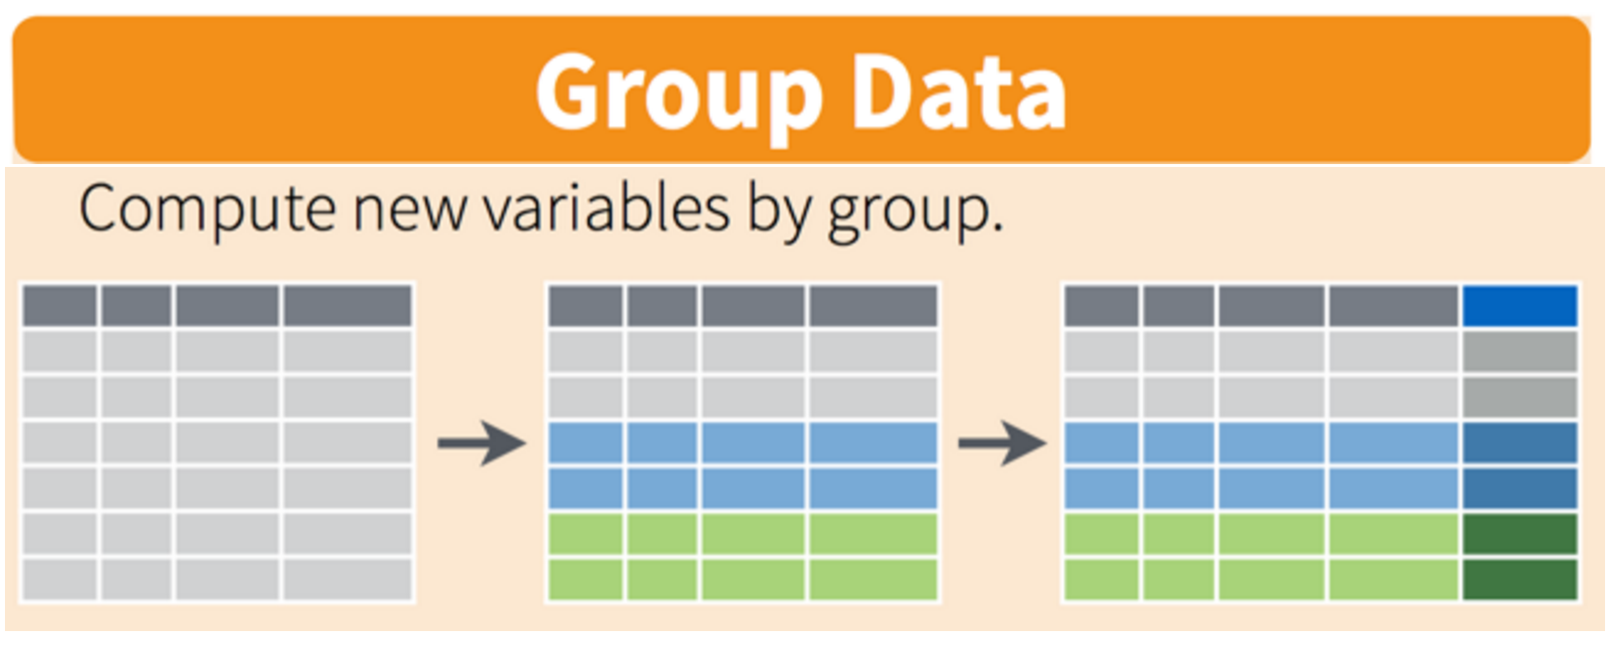
\includegraphics{img/rstudio-cheatsheet-group_by.png}
\caption{}
\end{figure}

\begin{Shaded}
\begin{Highlighting}[]
\NormalTok{gapminder %>%}
\StringTok{  }\KeywordTok{group_by}\NormalTok{(country) %>%}
\StringTok{  }\KeywordTok{mutate}\NormalTok{(}\DataTypeTok{gdp     =} \NormalTok{pop *}\StringTok{ }\NormalTok{gdpPercap,}
         \DataTypeTok{max_gdp =} \KeywordTok{max}\NormalTok{(gdp)) %>%}
\StringTok{  }\KeywordTok{ungroup}\NormalTok{() }\CommentTok{# if you use group_by, also use ungroup() to save heartache later}
\end{Highlighting}
\end{Shaded}

So instead of filtering for a specific country, we've grouped by
country, and then done the same operations. It's hard to see; let's look
at a bunch at the tail:

\begin{Shaded}
\begin{Highlighting}[]
\NormalTok{gapminder %>%}
\StringTok{  }\KeywordTok{group_by}\NormalTok{(country) %>%}
\StringTok{  }\KeywordTok{mutate}\NormalTok{(}\DataTypeTok{gdp     =} \NormalTok{pop *}\StringTok{ }\NormalTok{gdpPercap,}
         \DataTypeTok{max_gdp =} \KeywordTok{max}\NormalTok{(gdp)) %>%}
\StringTok{  }\KeywordTok{ungroup}\NormalTok{() %>%}\StringTok{ }
\StringTok{  }\KeywordTok{tail}\NormalTok{(}\DecValTok{30}\NormalTok{)}
\end{Highlighting}
\end{Shaded}

OK, this is great. But what if this what we needed, a max\_gdp value for
each country. We don't need that kind of repeated value for each of the
max\_gdp values. Here's the next function:

\subsection{\texorpdfstring{\texttt{dplyr::summarize()} with
\texttt{group\_by()}}{dplyr::summarize() with group\_by()}}\label{dplyrsummarize-with-group_by}

We want to operate on a group, but actually collapse or distill the
output from that group. The \texttt{summarize()} function will do that
for us.

Visually, we are doing this (thanks RStudio for your
\href{http://www.rstudio.com/wp-content/uploads/2015/02/data-wrangling-cheatsheet.pdf}{cheatsheet}):


\includegraphics{img/rstudio-cheatsheet-summarise.png} Here we go:

\begin{Shaded}
\begin{Highlighting}[]
\NormalTok{gapminder %>%}
\StringTok{  }\KeywordTok{group_by}\NormalTok{(country) %>%}
\StringTok{  }\KeywordTok{mutate}\NormalTok{(}\DataTypeTok{gdp =} \NormalTok{pop *}\StringTok{ }\NormalTok{gdpPercap) %>%}
\StringTok{  }\KeywordTok{summarize}\NormalTok{(}\DataTypeTok{max_gdp =} \KeywordTok{max}\NormalTok{(gdp)) %>%}
\StringTok{  }\KeywordTok{ungroup}\NormalTok{()}
\end{Highlighting}
\end{Shaded}

How cool is that! \texttt{summarize()} will actually only keep the
columns that are grouped\_by or summarized. So if we wanted to keep
other columns, we'd have to do it another way (we'll get into it
tomorrow).

\section{\texorpdfstring{\texttt{dplyr::arrange()} to
order}{dplyr::arrange() to order}}\label{dplyrarrange-to-order}

This is ordered alphabetically, which is cool. But let's say we wanted
to order it in ascending order for \texttt{max\_gdp}. The dplyr function
is \texttt{arrange()}.

\begin{Shaded}
\begin{Highlighting}[]
\NormalTok{gapminder %>%}
\StringTok{  }\KeywordTok{group_by}\NormalTok{(country) %>%}
\StringTok{  }\KeywordTok{mutate}\NormalTok{(}\DataTypeTok{gdp =} \NormalTok{pop *}\StringTok{ }\NormalTok{gdpPercap) %>%}
\StringTok{  }\KeywordTok{summarize}\NormalTok{(}\DataTypeTok{max_gdp =} \KeywordTok{max}\NormalTok{(gdp)) %>%}
\StringTok{  }\KeywordTok{ungroup}\NormalTok{() %>%}
\StringTok{  }\KeywordTok{arrange}\NormalTok{(max_gdp)}
\end{Highlighting}
\end{Shaded}

\section{Your turn}\label{your-turn-9}

Find the maximum gdpPercap of Egypt and Vietnam Create a new column.

Then, sync to Github.com (pull, stage, commit, push).

Do the following:

\begin{enumerate}
\def\labelenumi{\arabic{enumi}.}
\tightlist
\item
  arrange your data frame in descending order (opposite of what we've
  done). Expect that this is possible: use the Help pages.
\item
  save your data frame as a variable
\item
  Knit your RMarkdown file
\item
  Sync your .Rmd and .html to GitHub (pull, stage, commit, push)
\end{enumerate}

\subsection{Answer}\label{answer-2}

\ldots{}

\section{All together now}\label{all-together-now}

We have done a pretty incredible amount of work in a few lines. Our
whole analysis is this. Imagine the possibilities from here. It's very
readable: you see the data as the first thing, it's not nested. Then,
you can read the verbs. This is the whole thing, with explicit package
calls from \texttt{readr::} and \texttt{dplyr::}:

\begin{Shaded}
\begin{Highlighting}[]
\NormalTok{## gapminder-wrangle.R}
\NormalTok{## J. Lowndes lowndes@nceas.ucsb.edu}


\NormalTok{## load libraries}
\KeywordTok{library}\NormalTok{(tidyverse) ## install.packages('tidyverse')}

\NormalTok{## read in data}
\NormalTok{gapminder <-}\StringTok{ }\NormalTok{readr::}\KeywordTok{read_csv}\NormalTok{(}\StringTok{'https://raw.githubusercontent.com/jules32/2017-11-30-MBARI/gh-pages/data/gapminder.csv'}\NormalTok{) }

\NormalTok{## summarize}
\NormalTok{max_gdp <-}\StringTok{ }\NormalTok{gapminder %>%}\StringTok{ }
\StringTok{  }\NormalTok{dplyr::}\KeywordTok{select}\NormalTok{(-continent, -lifeExp) %>%}\StringTok{ }\CommentTok{# or select(country, year, pop, gdpPercap)}
\StringTok{  }\NormalTok{dplyr::}\KeywordTok{group_by}\NormalTok{(country) %>%}
\StringTok{  }\NormalTok{dplyr::}\KeywordTok{mutate}\NormalTok{(}\DataTypeTok{gdp =} \NormalTok{pop *}\StringTok{ }\NormalTok{gdpPercap) %>%}
\StringTok{  }\NormalTok{dplyr::}\KeywordTok{summarize}\NormalTok{(}\DataTypeTok{max_gdp =} \KeywordTok{max}\NormalTok{(gdp)) %>%}
\StringTok{  }\NormalTok{dplyr::}\KeywordTok{ungroup}\NormalTok{() }
\end{Highlighting}
\end{Shaded}

I actually am borrowing this ``All together now'' from Tony Fischetti's
blog post
\href{http://www.statsblogs.com/2014/02/10/how-dplyr-replaced-my-most-common-r-idioms/}{How
dplyr replaced my most common R idioms}). With that as inspiration, this
is how what we have just done would look like in Base R.

\subsection{Compare to base R}\label{compare-to-base-r}

Let's compare with some base R code to accomplish the same things. Base
R requires subsetting with the \texttt{{[}rows,\ columns{]}} notatation.
This notation is something you'll see a lot in base R. the brackets
\texttt{{[}\ {]}} allow you to extract parts of an object. Within the
brackets, the comma separates rows from columns.

If we don't write anything after the comma, that means ``all columns''.
And if we don't write anything before the comma, that means ``all
rows''.

Also, the \texttt{\$} operator is how you access specific columns of
your dataframe. You can also add new columns like we do with
\texttt{mex\$gdp}.

Here we will just calculate the max for one country, Mexico. Tomorrow we
will learn how to do it for all the countries, like we did with
\texttt{dplyr::group\_by()}.

\begin{Shaded}
\begin{Highlighting}[]
\NormalTok{## gapminder-wrangle.R --- baseR}
\NormalTok{## J. Lowndes lowndes@nceas.ucsb.edu}

\NormalTok{## Note the stringAsFactors = FALSE variable to avoid factors!}
\NormalTok{gapminder <-}\StringTok{ }\KeywordTok{read.csv}\NormalTok{(}\StringTok{'https://raw.githubusercontent.com/jules32/2017-11-30-MBARI/gh-pages/data/gapminder.csv'}\NormalTok{, }\DataTypeTok{stringsAsFactors =} \OtherTok{FALSE}\NormalTok{) }

\NormalTok{## subsetting columns. Compare to `dplyr::select()`}
\NormalTok{x1  <-}\StringTok{ }\NormalTok{gapminder[ , }\KeywordTok{c}\NormalTok{(}\StringTok{'country'}\NormalTok{, }\StringTok{'year'}\NormalTok{, }\StringTok{'pop'}\NormalTok{, }\StringTok{'gdpPercap'}\NormalTok{) ]}

\NormalTok{## subsetting rows. Compare to `dplyr::filter()`}
\NormalTok{mex <-}\StringTok{ }\NormalTok{x1[x1$country ==}\StringTok{ "Mexico"}\NormalTok{, ]}

\NormalTok{## adding new columns. Compare to `dplyr::mutate()`. }
\NormalTok{mex$gdp <-}\StringTok{ }\NormalTok{mex$pop *}\StringTok{ }\NormalTok{mex$gdpPercap}
\NormalTok{mex$max_gdp <-}\StringTok{ }\KeywordTok{max}\NormalTok{(mex$gdp)}
\end{Highlighting}
\end{Shaded}

Note too that the chain operator \texttt{\%\textgreater{}\%} that we
used with the \texttt{tidyverse} lets us get away from the temporary
variable x1.

\section{Your Turn}\label{your-turn-10}

Get your RMarkdown file cleaned up and sync it for the last time today!

\subsection{Answers}\label{answers}

\ldots{}

\section{Key Points}\label{key-points}

\begin{itemize}
\tightlist
\item
  Data manipulation functions in \texttt{dplyr} allow you to
  \texttt{filter()} by rows and \texttt{select()} by columns, create new
  columns with \texttt{mutate()}, and \texttt{group\_by()} unique column
  values to apply \texttt{summarize()} for new columns that define
  aggregate values across groupings.
\item
  The ``then'' operator \texttt{\%\textgreater{}\%} allows you to chain
  successive operations without needing to define intermediary variables
  for creating the most parsimonious, easily read analysis.
\end{itemize}

\chapter{Wrangling (tidyr)}\label{tidyr}

\section{Objectives \& Resources}\label{objectives-resources-3}

\textbf{Objectives}

\begin{itemize}
\tightlist
\item
  learn tidyr with gapminder package
\item
  other wrangling: joins, bind\_cols (see
  \url{http://r4ds.had.co.nz/relational-data})
\item
  practice RStudio-GitHub workflow
\item
  your turn: use the data wrangling cheat sheet to explore window
  functions
\end{itemize}

\textbf{Resources}

\section{\texorpdfstring{\texttt{tidyr}
overview}{tidyr overview}}\label{tidyr-overview}

Often, data must be reshaped for it to become tidy data. What does that
mean? There are four main verbs we'll use, which are essentially pairs
of opposites:

\begin{itemize}
\tightlist
\item
  turn columns into rows (\texttt{gather()}),
\item
  turn rows into columns (\texttt{spread()}),
\item
  turn a character column into multiple columns (\texttt{separate()}),
\item
  turn multiple character columns into a single column
  (\texttt{unite()})
\end{itemize}

\begin{figure}[htbp]
\centering
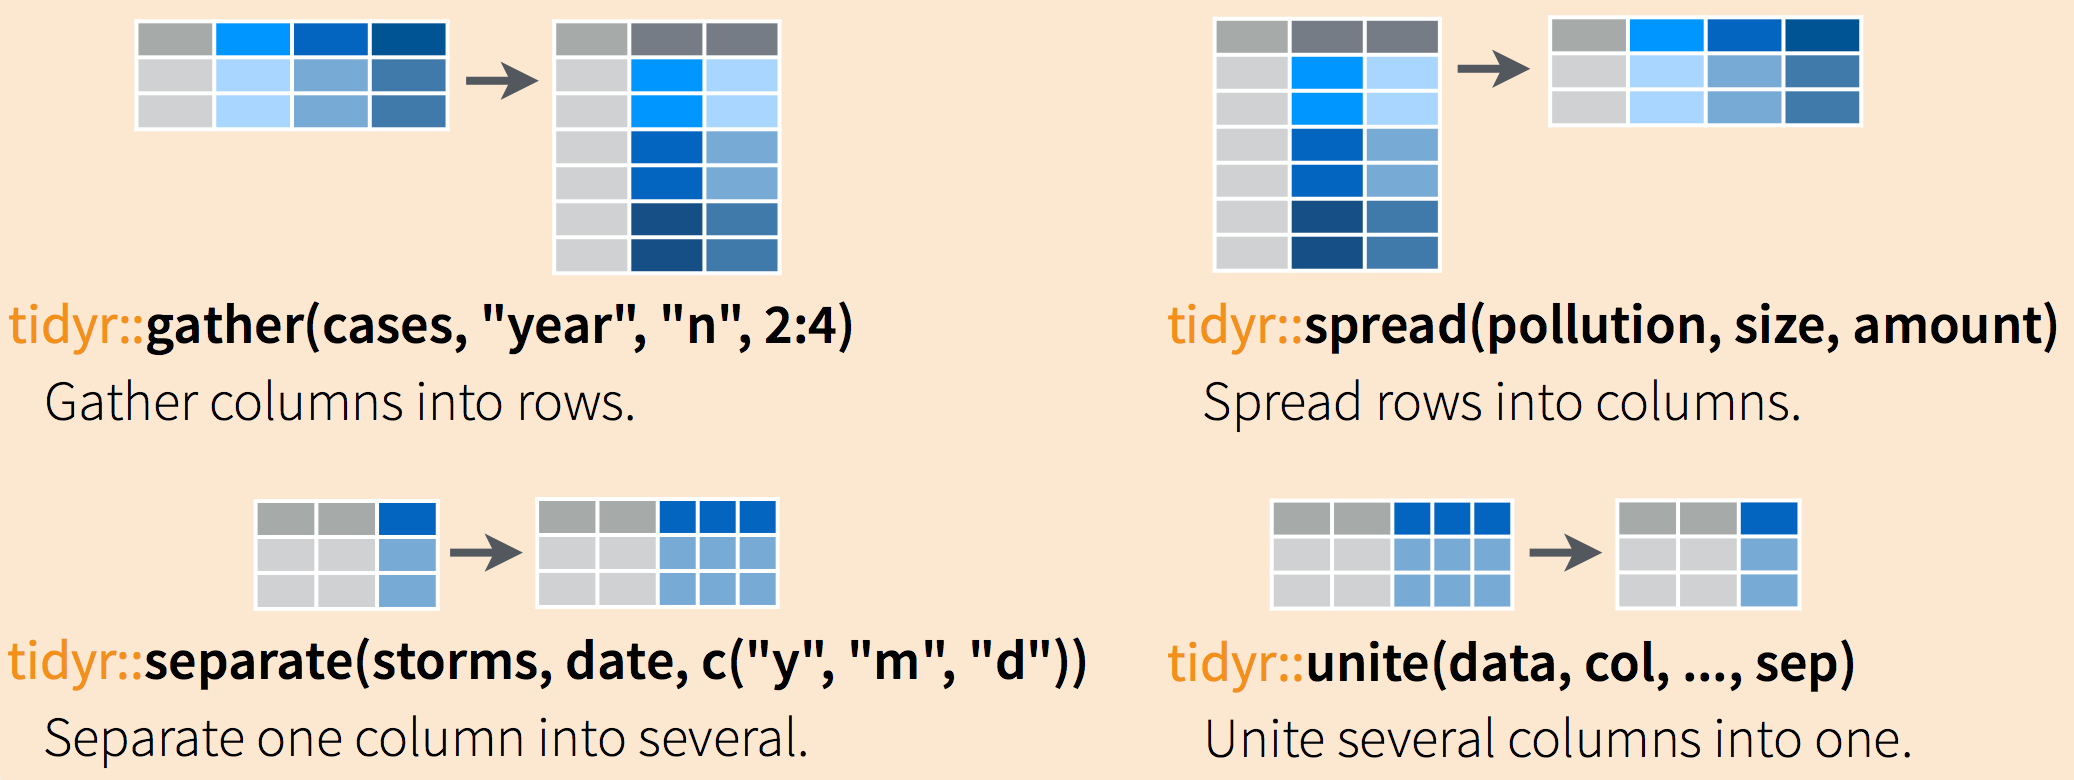
\includegraphics{img/rstudio-cheatsheet-spread-gather-sep-unite.png}
\caption{}
\end{figure}

You use \texttt{spread()} and \texttt{gather()} to transform or reshape
data between `wide' to `long' formats. `long' format is the tidy data we
are after, where:

\begin{itemize}
\tightlist
\item
  each column is a variable
\item
  each row is an observation
\end{itemize}

In the `long' format, you usually have 1 column for the observed
variable and the other columns are ID variables.

For the `wide' format each row is often a site/subject/patient and you
have multiple observation variables containing the same type of data.
These can be either repeated observations over time, or observation of
multiple variables (or a mix of both). Data input may be simpler or some
other applications may prefer the `wide' format. However, many of
\texttt{R}`s functions have been designed assuming you have 'long'
format data.

These data formats mainly affect readability. For humans, the wide
format is often more intuitive since we can often see more of the data
on the screen due to it's shape. However, the long format is more
machine readable and is closer to the formatting of databases. The ID
variables in our dataframes are similar to the fields in a database and
observed variables are like the database values.

\begin{quote}
Question: Is gapminder a purely long, purely wide, or some intermediate
format?
\end{quote}

Sometimes, as with the gapminder dataset, we have multiple types of
observed data. It is somewhere in between the purely `long' and `wide'
data formats:

\begin{itemize}
\tightlist
\item
  3 ``ID variables'' (\texttt{continent}, \texttt{country},
  \texttt{year})
\item
  3 ``Observation variables''
  (\texttt{pop},\texttt{lifeExp},\texttt{gdpPercap}).
\end{itemize}

It's pretty common to have data in this intermediate format in most
cases despite not having ALL observations in 1 column, since all 3
observation variables have different units. But we can play with
switching it to long format and wide to show what that means (i.e.~long
would be 4 ID variables and 1 Observation variable).

\textbf{Note:} Generally, mathematical operations are better in long
format, although some plotting functions actually work better with wide
format.

\subsection{\texorpdfstring{Install \texttt{tidyr}, investigate
gapminder
data}{Install tidyr, investigate gapminder data}}\label{install-tidyr-investigate-gapminder-data}

First install and load \texttt{tidyr}:

\begin{Shaded}
\begin{Highlighting}[]
\CommentTok{#install.packages("tidyr")}
\KeywordTok{library}\NormalTok{(}\StringTok{"tidyr"}\NormalTok{) }\CommentTok{# warning messages are OK}
\end{Highlighting}
\end{Shaded}

\section{\texorpdfstring{From wide to long format with
\texttt{gather()}}{From wide to long format with gather()}}\label{from-wide-to-long-format-with-gather}

We've been working with pretty tidy data. So for practice, now let's
work with these data in a wider format, maybe the way you or your
colleague entered it in a spreadsheet. We'll work with it to get it back
to the way we like it.

\begin{Shaded}
\begin{Highlighting}[]
\NormalTok{gap_wide <-}\StringTok{ }\KeywordTok{read.csv}\NormalTok{(}\StringTok{'data/gapminder_wide.csv'}\NormalTok{)}
\end{Highlighting}
\end{Shaded}

\begin{Shaded}
\begin{Highlighting}[]
\KeywordTok{head}\NormalTok{(gap_wide)}
\KeywordTok{str}\NormalTok{(gap_wide)}
\end{Highlighting}
\end{Shaded}

While wide format is nice for data entry, it's not nice for
calculations. What if you were asked for the mean population after 1990
in Algeria? Possible, but ugly. Let's tidy it back to the intermediate
format we've been using.

\begin{quote}
Question: let's talk this through together. If we're trying to turn the
\texttt{gap\_wide} format into \texttt{gapminder} format, what structure
does it have that we like? And that we want to change?
\end{quote}

\begin{itemize}
\tightlist
\item
  We like the continent and country columns. We won't want to change
  those.
\item
  For long format, we'd want just 1 column identifying the variable name
  (\texttt{tidyr} calls this a \textbf{`key'}), and 1 column for the
  data (\texttt{tidyr} calls this the '\textbf{value'}).
\item
  For intermediate format, we'd want 3 columns for \texttt{gdpPercap},
  \texttt{lifeExp}, and \texttt{pop}.
\item
  We would like year as a separate column.
\end{itemize}

Let's get it to long format. We'll have to do this in 2 steps. The first
step is to take all of those column names and make them a variable in a
new column, and transfer the values into another column.

Let's have a look at \texttt{gather()}'s help:

\begin{Shaded}
\begin{Highlighting}[]
\NormalTok{?gather}
\end{Highlighting}
\end{Shaded}

\begin{quote}
Question: What is our \textbf{key-value pair}?
\end{quote}

We need to name two new variables in the key-value pair, one for the
key, one for the value. Let's name them \texttt{obstype\_year} and
\texttt{obs\_value}.

Here's the start of what we'll do:

\begin{Shaded}
\begin{Highlighting}[]
\NormalTok{gap_long <-}\StringTok{ }\NormalTok{gap_wide %>%}\StringTok{ }
\StringTok{  }\KeywordTok{gather}\NormalTok{(}\DataTypeTok{key   =} \NormalTok{obstype_year,}
         \DataTypeTok{value =} \NormalTok{obs_values)}
\end{Highlighting}
\end{Shaded}

\begin{Shaded}
\begin{Highlighting}[]
\KeywordTok{str}\NormalTok{(gap_long)}
\KeywordTok{head}\NormalTok{(gap_long)}
\KeywordTok{tail}\NormalTok{(gap_long)}
\end{Highlighting}
\end{Shaded}

So this has reshaped our dataframe, but really not how we wanted. Very
important to check, and listen to that warning message--dropping
attributes seems very suspicious. Like suspenders.

What went wrong? Notice that it didn't know that we wanted to keep
\texttt{continent} and \texttt{country} untouched; we need to give it
more information about which columns we want reshaped. We can do this in
several ways.

One way: identify the column numbers you want to use. Not ideal because
column numbers could change, but it does exactly what we want! And
illustrates it nicely.

\begin{Shaded}
\begin{Highlighting}[]
\NormalTok{gap_long <-}\StringTok{ }\NormalTok{gap_wide %>%}\StringTok{ }
\StringTok{  }\KeywordTok{gather}\NormalTok{(}\DataTypeTok{key   =} \NormalTok{obstype_year,}
         \DataTypeTok{value =} \NormalTok{obs_values,}
         \DecValTok{3}\NormalTok{:}\DecValTok{38}\NormalTok{)  }\CommentTok{# could also do -1, -2: 'not column one, not column two}
\KeywordTok{str}\NormalTok{(gap_long)}
\KeywordTok{head}\NormalTok{(gap_long)}
\KeywordTok{tail}\NormalTok{(gap_long)}
\end{Highlighting}
\end{Shaded}

Better way: identify the columns by name. Listing them out by explicit
name can be a good approach if there are a few. But I'm not going to
list them out here, and way too much potential for error if you tried
gdpPercap\_1952, gdpPercap\_1957, gdpPercap\_1962\ldots{} So let's use
some of \texttt{dplyr}'s awesome helper functions.

\begin{Shaded}
\begin{Highlighting}[]
\NormalTok{gap_long <-}\StringTok{ }\NormalTok{gap_wide %>%}\StringTok{ }
\StringTok{  }\KeywordTok{gather}\NormalTok{(}\DataTypeTok{key   =} \NormalTok{obstype_year,}
         \DataTypeTok{value =} \NormalTok{obs_values,}
         \NormalTok{dplyr::}\KeywordTok{starts_with}\NormalTok{(}\StringTok{'pop'}\NormalTok{),}
         \NormalTok{dplyr::}\KeywordTok{starts_with}\NormalTok{(}\StringTok{'lifeExp'}\NormalTok{),}
         \NormalTok{dplyr::}\KeywordTok{starts_with}\NormalTok{(}\StringTok{'gdpPercap'}\NormalTok{))}
\KeywordTok{str}\NormalTok{(gap_long)}
\KeywordTok{head}\NormalTok{(gap_long)}
\KeywordTok{tail}\NormalTok{(gap_long)}
\end{Highlighting}
\end{Shaded}

Success! And you could also do it this way.

\begin{Shaded}
\begin{Highlighting}[]
\NormalTok{gap_long <-}\StringTok{ }\NormalTok{gap_wide %>%}\StringTok{ }
\StringTok{  }\KeywordTok{gather}\NormalTok{(}\DataTypeTok{key   =} \NormalTok{obstype_year,}
         \DataTypeTok{value =} \NormalTok{obs_values,}
         \NormalTok{-continent, -country)}
\KeywordTok{str}\NormalTok{(gap_long)}
\KeywordTok{head}\NormalTok{(gap_long)}
\KeywordTok{tail}\NormalTok{(gap_long)}
\end{Highlighting}
\end{Shaded}

To recap:

Inside \texttt{gather()} we first name the new column for the new ID
variable (\texttt{obstype\_year}), the name for the new amalgamated
observation variable (\texttt{obs\_value}), then the names of the old
observation variable. We could have typed out all the observation
variables, but as in the \texttt{select()} function (see \texttt{dplyr}
lesson), we can use the \texttt{starts\_with()} argument to select all
variables that starts with the desired character string. Gather also
allows the alternative syntax of using the \texttt{-} symbol to identify
which variables are not to be gathered (i.e.~ID variables)

OK, but we're not done yet. \texttt{obstype\_year} actually contains 2
pieces of information, the observation type
(\texttt{pop},\texttt{lifeExp}, or \texttt{gdpPercap}) and the
\texttt{year}. We can use the \texttt{separate()} function to split the
character strings into multiple variables

\texttt{?separate} --\textgreater{} we'll tell it which column we want
separated, name new columns that we want to create, and tell it what we
want it to separate by. Since the \texttt{obstype\_year} variable has
observation types and years separated by a \texttt{\_}, we'll use that.

\begin{Shaded}
\begin{Highlighting}[]
\NormalTok{gap_long <-}\StringTok{ }\NormalTok{gap_wide %>%}\StringTok{ }
\StringTok{  }\KeywordTok{gather}\NormalTok{(}\DataTypeTok{key   =} \NormalTok{obstype_year,}
         \DataTypeTok{value =} \NormalTok{obs_values,}
         \NormalTok{-continent, -country) %>%}
\StringTok{  }\KeywordTok{separate}\NormalTok{(obstype_year,}
           \DataTypeTok{into =} \KeywordTok{c}\NormalTok{(}\StringTok{'obs_type'}\NormalTok{,}\StringTok{'year'}\NormalTok{),}
           \DataTypeTok{sep=}\StringTok{"_"}\NormalTok{)}
\end{Highlighting}
\end{Shaded}

\begin{Shaded}
\begin{Highlighting}[]
\KeywordTok{str}\NormalTok{(gap_long)}
\KeywordTok{head}\NormalTok{(gap_long)}
\KeywordTok{tail}\NormalTok{(gap_long)}
\end{Highlighting}
\end{Shaded}

Excellent. This is long format: every row is a unique observation. Yay!

\begin{quote}
Exercise: Using \texttt{gap\_long}, calculate the mean life expectancy,
population, and gdpPercap for each continent. \textbf{Hint:} use the
\texttt{group\_by()} and \texttt{summarize()} functions we learned in
the \texttt{dplyr} lesson
\end{quote}

\begin{Shaded}
\begin{Highlighting}[]
\CommentTok{# solution (no peeking!)}
\NormalTok{gap_long %>%}\StringTok{ }
\StringTok{  }\KeywordTok{group_by}\NormalTok{(continent, obs_type) %>%}
\StringTok{    }\KeywordTok{summarize}\NormalTok{(}\DataTypeTok{means =} \KeywordTok{mean}\NormalTok{(obs_values))}
\end{Highlighting}
\end{Shaded}

\section{\texorpdfstring{From long to intermediate format with
\texttt{spread()}}{From long to intermediate format with spread()}}\label{from-long-to-intermediate-format-with-spread}

\begin{figure}[htbp]
\centering
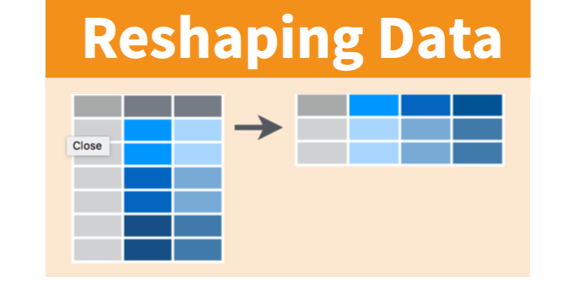
\includegraphics{img/rstudio-cheatsheet-reshaping-data-spread.png}
\caption{}
\end{figure}

Now just to double-check our work, let's use the opposite of
\texttt{gather()} to spread our observation variables back to the
original format with the aptly named \texttt{spread()}. You pass
\texttt{spread()} the key and value pair, which is now
\texttt{obs\_type} and \texttt{obs\_values}.

\begin{Shaded}
\begin{Highlighting}[]
\NormalTok{gap_normal <-}\StringTok{ }\NormalTok{gap_long %>%}\StringTok{ }
\StringTok{  }\KeywordTok{spread}\NormalTok{(obs_type, obs_values)}
\end{Highlighting}
\end{Shaded}

\begin{Shaded}
\begin{Highlighting}[]
\KeywordTok{dim}\NormalTok{(gap_normal)}
\KeywordTok{dim}\NormalTok{(gapminder)}
\KeywordTok{names}\NormalTok{(gap_normal)}
\KeywordTok{names}\NormalTok{(gapminder)}
\end{Highlighting}
\end{Shaded}

Now we've got an intermediate dataframe \texttt{gap\_normal} with the
same dimensions as the original \texttt{gapminder}, but the order of the
variables is different. Let's fix that before checking if they are
\texttt{all.equal()}.

\begin{quote}
Exercise: reorder the columns in gap\_normal to match gapminder.
\end{quote}

\begin{Shaded}
\begin{Highlighting}[]
\CommentTok{# Solution, no peeking!}

\CommentTok{# one way with dplyr (also nice because can chain this from gap_normal creation)}
\NormalTok{gap_normal <-}\StringTok{ }\NormalTok{gap_normal %>%}
\StringTok{  }\KeywordTok{select}\NormalTok{(country, continent, year, lifeExp, pop, gdpPercap)}

\CommentTok{# another way with base R}
\NormalTok{gap_normal <-}\StringTok{ }\NormalTok{gap_normal[,}\KeywordTok{names}\NormalTok{(gapminder)]}
\end{Highlighting}
\end{Shaded}

Now let's check if they are all.equal (\texttt{?all.equal}) is a handy
test

\begin{Shaded}
\begin{Highlighting}[]
\KeywordTok{all.equal}\NormalTok{(gap_normal,gapminder)}
\end{Highlighting}
\end{Shaded}

\begin{Shaded}
\begin{Highlighting}[]
\KeywordTok{head}\NormalTok{(gap_normal)}
\KeywordTok{head}\NormalTok{(gapminder)}
\end{Highlighting}
\end{Shaded}

We're almost there, the original was sorted by \texttt{country},
\texttt{continent}, then \texttt{year}.

\begin{Shaded}
\begin{Highlighting}[]
\NormalTok{gap_normal <-}\StringTok{ }\NormalTok{gap_normal %>%}\StringTok{ }\KeywordTok{arrange}\NormalTok{(country,continent,year)}
\KeywordTok{all.equal}\NormalTok{(gap_normal,gapminder)}
\end{Highlighting}
\end{Shaded}

\begin{Shaded}
\begin{Highlighting}[]
\KeywordTok{str}\NormalTok{(gap_normal)}
\KeywordTok{str}\NormalTok{(gapminder)}
\end{Highlighting}
\end{Shaded}

Mine shows a slight difference because one is a data.frame and one is a
tbl\_df, which is similar to a data.frame. We won't get into this
difference now, I'm feeling good about these data sets! We've gone from
the longest format back to the intermediate and we didn't introduce any
errors in our code.

\begin{quote}
Exercise: convert gap\_long all the way back to gap\_wide. Hint: you'll
need to create appropriate labels for all our new variables (time*metric
combinations) with \texttt{tidyr::unite()}.
\end{quote}

\begin{Shaded}
\begin{Highlighting}[]
\CommentTok{# Solution, no peeking: }
\KeywordTok{head}\NormalTok{(gap_long) }\CommentTok{# remember the columns}

\NormalTok{gap_wide_new <-}\StringTok{ }\NormalTok{gap_long %>%}\StringTok{ }
\StringTok{  }\CommentTok{# first unite obs_type and year into a new column called var_names. Separate by _}
\StringTok{  }\KeywordTok{unite}\NormalTok{(}\DataTypeTok{col =} \NormalTok{var_names, obs_type, year, }\DataTypeTok{sep =} \StringTok{"_"}\NormalTok{) %>%}\StringTok{ }
\StringTok{  }\CommentTok{# then spread var_names out by key-value pair.}
\StringTok{  }\KeywordTok{spread}\NormalTok{(}\DataTypeTok{key =} \NormalTok{var_names, }\DataTypeTok{value =} \NormalTok{obs_values)}
\KeywordTok{str}\NormalTok{(gap_wide_new)}
\end{Highlighting}
\end{Shaded}

\subsection{clean up and save your .r
script}\label{clean-up-and-save-your-.r-script}

Spend some time cleaning up and saving \texttt{gapminder-wrangle.r}
Restart R. In RStudio, use \emph{Session \textgreater{} Restart R}.
Otherwise, quit R with \texttt{q()} and re-launch it.

Your final R script could look something like this:

\begin{Shaded}
\begin{Highlighting}[]
\NormalTok{## install, load dplyr}
\CommentTok{#install.packages("dplyr") ## do this once only to install the package on your computer.}
\KeywordTok{library}\NormalTok{(dplyr)}

\NormalTok{## load gapminder}
\KeywordTok{library}\NormalTok{(gapminder) }\CommentTok{# this is the package name}
\KeywordTok{str}\NormalTok{(gapminder) }\CommentTok{# there's still a data frame named 'gapminder'}

\NormalTok{## practice dplyr::filter()}
\KeywordTok{filter}\NormalTok{(gapminder, lifeExp <}\StringTok{ }\DecValTok{29}\NormalTok{)}
\KeywordTok{filter}\NormalTok{(gapminder, country ==}\StringTok{ "Mexico"}\NormalTok{)}
\KeywordTok{filter}\NormalTok{(gapminder, country %in%}\StringTok{ }\KeywordTok{c}\NormalTok{(}\StringTok{"Mexico"}\NormalTok{, }\StringTok{"Afghanistan"}\NormalTok{))}

\NormalTok{## base R alternatives to dplyr::filter()}
\NormalTok{gapminder[gapminder$lifeExp <}\StringTok{ }\DecValTok{29}\NormalTok{, ] ## repeat `gapminder`, [i, j] indexing is distracting}
\KeywordTok{subset}\NormalTok{(gapminder, country ==}\StringTok{ "Mexico"}\NormalTok{) ## almost same as filter ... but wait ...}

\NormalTok{## pipe operator %>%}
\NormalTok{gapminder %>%}\StringTok{ }\NormalTok{head }\CommentTok{# this...}
\KeywordTok{head}\NormalTok{(gapminder) }\CommentTok{# ...is the same as this!}
\NormalTok{gapminder %>%}\StringTok{ }\KeywordTok{head}\NormalTok{(}\DecValTok{3}\NormalTok{) }\CommentTok{# can pass arguments! this...}
\KeywordTok{head}\NormalTok{(gapminder, }\DecValTok{3}\NormalTok{) }\CommentTok{# ...is the same as this!}

\NormalTok{## practice dplyr::select() with %>%}
\KeywordTok{select}\NormalTok{(gapminder, year, lifeExp) }\CommentTok{# this...}
\NormalTok{gapminder %>%}\StringTok{ }\KeywordTok{select}\NormalTok{(year, lifeExp) }\CommentTok{# ...is the same as this!}

\NormalTok{## practice with %>% chains}
\NormalTok{gapminder %>%}
\StringTok{  }\KeywordTok{select}\NormalTok{(year, lifeExp) %>%}\StringTok{ }
\StringTok{  }\KeywordTok{head}\NormalTok{(}\DecValTok{4}\NormalTok{) }\CommentTok{# doesn't have to be a dplyr function}

\NormalTok{gapminder %>%}
\StringTok{  }\KeywordTok{filter}\NormalTok{(country ==}\StringTok{ "Cambodia"}\NormalTok{) %>%}
\StringTok{  }\KeywordTok{select}\NormalTok{(-continent, -lifeExp) }\CommentTok{# same as select(country, year, pop, gdpPercap) }

\CommentTok{# compare to base R, hard to read!}
\NormalTok{gapminder[gapminder$country ==}\StringTok{ "Cambodia"}\NormalTok{, }\KeywordTok{c}\NormalTok{(}\StringTok{"country"}\NormalTok{, }\StringTok{"year"}\NormalTok{, }\StringTok{"pop"}\NormalTok{, }\StringTok{"gdpPercap"}\NormalTok{)]}
\KeywordTok{subset}\NormalTok{(gapminder, country ==}\StringTok{ "Cambodia"}\NormalTok{, }\DataTypeTok{select =} \KeywordTok{c}\NormalTok{(country, year, pop, gdpPercap))}

\NormalTok{## dplyr::mutate() adds new columns}
\NormalTok{gapminder %>%}
\StringTok{  }\KeywordTok{filter}\NormalTok{(country ==}\StringTok{ "Cambodia"}\NormalTok{) %>%}
\StringTok{  }\KeywordTok{select}\NormalTok{(-continent, -lifeExp) %>%}
\StringTok{  }\KeywordTok{mutate}\NormalTok{(}\DataTypeTok{gdp =} \NormalTok{pop *}\StringTok{ }\NormalTok{gdpPercap)}

\NormalTok{## dplyr::summarize() or summarise() adds new column when grouping}
\NormalTok{gapminder %>%}
\StringTok{  }\KeywordTok{filter}\NormalTok{(country ==}\StringTok{ "Cambodia"}\NormalTok{) %>%}
\StringTok{  }\KeywordTok{select}\NormalTok{(-continent, -lifeExp) %>%}
\StringTok{  }\KeywordTok{mutate}\NormalTok{(}\DataTypeTok{gdp =} \NormalTok{pop *}\StringTok{ }\NormalTok{gdpPercap) %>%}
\StringTok{  }\KeywordTok{group_by}\NormalTok{(country) %>%}
\StringTok{  }\KeywordTok{summarize}\NormalTok{(}\DataTypeTok{mean_gdp =} \KeywordTok{mean}\NormalTok{(gdp)) %>%}
\StringTok{  }\KeywordTok{ungroup}\NormalTok{() }\CommentTok{# if you use group_by, also use ungroup() to save heartache later}

\NormalTok{## summarize for all countries (replaces our for loop!)}
\NormalTok{gapminder %>%}
\StringTok{  }\KeywordTok{select}\NormalTok{(-continent, -lifeExp) %>%}
\StringTok{  }\KeywordTok{mutate}\NormalTok{(}\DataTypeTok{gdp =} \NormalTok{pop *}\StringTok{ }\NormalTok{gdpPercap) %>%}
\StringTok{  }\KeywordTok{group_by}\NormalTok{(country) %>%}
\StringTok{  }\KeywordTok{summarize}\NormalTok{(}\DataTypeTok{mean_gdp =} \KeywordTok{mean}\NormalTok{(gdp)) %>%}
\StringTok{  }\KeywordTok{ungroup}\NormalTok{() }\CommentTok{# if you use group_by, also use ungroup() to save heartache later}

\NormalTok{## install tidyr}
\KeywordTok{install.packages}\NormalTok{(}\StringTok{"tidyr"}\NormalTok{)}
\KeywordTok{library}\NormalTok{(tidyr)}

\NormalTok{## load wide data}
\NormalTok{gap_wide <-}\StringTok{ }\KeywordTok{read.csv}\NormalTok{(}\StringTok{'data/gapminder_wide.csv'}\NormalTok{)}
\KeywordTok{head}\NormalTok{(gap_wide)}
\KeywordTok{str}\NormalTok{(gap_wide)}

\NormalTok{## practice tidyr::gather() wide to long}
\NormalTok{gap_long <-}\StringTok{ }\NormalTok{gap_wide %>%}\StringTok{ }
\StringTok{  }\KeywordTok{gather}\NormalTok{(}\DataTypeTok{key   =} \NormalTok{obstype_year,}
         \DataTypeTok{value =} \NormalTok{obs_values,}
         \NormalTok{-continent, -country) }
\CommentTok{# or }
\NormalTok{gap_long <-}\StringTok{ }\NormalTok{gap_wide %>%}\StringTok{ }
\StringTok{  }\KeywordTok{gather}\NormalTok{(}\DataTypeTok{key   =} \NormalTok{obstype_year,}
         \DataTypeTok{value =} \NormalTok{obs_values,}
         \NormalTok{dplyr::}\KeywordTok{starts_with}\NormalTok{(}\StringTok{'pop'}\NormalTok{),}
         \NormalTok{dplyr::}\KeywordTok{starts_with}\NormalTok{(}\StringTok{'lifeExp'}\NormalTok{),}
         \NormalTok{dplyr::}\KeywordTok{starts_with}\NormalTok{(}\StringTok{'gdpPercap'}\NormalTok{))}
\CommentTok{# or (but always be wary of numerics because they could change silently)}
\NormalTok{gap_long <-}\StringTok{ }\NormalTok{gap_wide %>%}\StringTok{ }
\StringTok{  }\KeywordTok{gather}\NormalTok{(}\DataTypeTok{key   =} \NormalTok{obstype_year,}
         \DataTypeTok{value =} \NormalTok{obs_values,}
         \DecValTok{3}\NormalTok{:}\DecValTok{38}\NormalTok{)  }\CommentTok{# could also do -1, -2: 'not column one, not column two}


\NormalTok{## gather() and separate() to create our original gapminder}
\NormalTok{gap_long <-}\StringTok{ }\NormalTok{gap_wide %>%}\StringTok{ }
\StringTok{  }\KeywordTok{gather}\NormalTok{(}\DataTypeTok{key   =} \NormalTok{obstype_year,}
         \DataTypeTok{value =} \NormalTok{obs_values,}
         \NormalTok{-continent, -country) %>%}
\StringTok{  }\KeywordTok{separate}\NormalTok{(obstype_year,}
           \DataTypeTok{into =} \KeywordTok{c}\NormalTok{(}\StringTok{'obs_type'}\NormalTok{,}\StringTok{'year'}\NormalTok{),}
           \DataTypeTok{sep=}\StringTok{"_"}\NormalTok{)}

\NormalTok{## practice: can still do calculations in long format}
\NormalTok{gap_long %>%}\StringTok{ }
\StringTok{  }\KeywordTok{group_by}\NormalTok{(continent, obs_type) %>%}
\StringTok{  }\KeywordTok{summarize}\NormalTok{(}\DataTypeTok{means =} \KeywordTok{mean}\NormalTok{(obs_values))}

\NormalTok{## spread() from normal to wide}
\NormalTok{gap_normal <-}\StringTok{ }\NormalTok{gap_long %>%}\StringTok{ }
\StringTok{  }\KeywordTok{spread}\NormalTok{(obs_type, obs_values) %>%}
\StringTok{  }\KeywordTok{select}\NormalTok{(country, continent, year, lifeExp, pop, gdpPercap)}
\CommentTok{# or }
\NormalTok{gap_normal <-}\StringTok{ }\NormalTok{gap_long %>%}\StringTok{ }
\StringTok{  }\KeywordTok{spread}\NormalTok{(obs_type, obs_values)}
\NormalTok{gap_normal <-}\StringTok{ }\NormalTok{gap_normal[,}\KeywordTok{names}\NormalTok{(gapminder)]}

\NormalTok{## check that all.equal()}
\KeywordTok{all.equal}\NormalTok{(gap_normal,gapminder)}

\NormalTok{## unite() and spread(): convert gap_long to gap_wide}
\KeywordTok{head}\NormalTok{(gap_long) }\CommentTok{# remember the columns}

\NormalTok{gap_wide_new <-}\StringTok{ }\NormalTok{gap_long %>%}\StringTok{ }
\StringTok{  }\CommentTok{# first unite obs_type and year into a new column called var_names. Separate by _}
\StringTok{  }\KeywordTok{unite}\NormalTok{(}\DataTypeTok{col =} \NormalTok{var_names, obs_type, year, }\DataTypeTok{sep =} \StringTok{"_"}\NormalTok{) %>%}\StringTok{ }
\StringTok{  }\CommentTok{# then spread var_names out by key-value pair.}
\StringTok{  }\KeywordTok{spread}\NormalTok{(}\DataTypeTok{key =} \NormalTok{var_names, }\DataTypeTok{value =} \NormalTok{obs_values)}
\KeywordTok{str}\NormalTok{(gap_wide_new)}
\end{Highlighting}
\end{Shaded}

\subsection{Other tidyr awesomeness}\label{other-tidyr-awesomeness}

\begin{itemize}
\tightlist
\item
  \texttt{complete()}
\end{itemize}

\begin{center}\rule{0.5\linewidth}{\linethickness}\end{center}

\section{Other links}\label{other-links}

\begin{itemize}
\tightlist
\item
  \href{http://ucsb-bren.github.io/env-info/wk04_tidyr.html}{Tidying up
  Data - Env Info} -
  \href{https://github.com/ucsb-bren/env-info/blob/gh-pages/wk04_tidyr.Rmd}{Rmd}
\item
  \href{http://bbest.github.io/dplyr-tidyr-tutorial/}{Data wrangling
  with dplyr and tidyr - Tyler Clavelle \& Dan Ovando} -
  \href{https://github.com/bbest/dplyr-tidyr-tutorial/blob/gh-pages/index.Rmd}{Rmd}
\end{itemize}

\section{Your turn}\label{your-turn-11}

ggplot2

\section{Troubleshooting}\label{troubleshooting-3}

\chapter{Analysis, continued}\label{analysis}

\section{Objectives and Resources}\label{objectives-and-resources}

\textbf{Objectives}

exposure and lots of practice:

Do a little analysis: for a continent, loop through and make figs, save
them each.

\begin{itemize}
\item
  importing and writing data

  \begin{itemize}
  \tightlist
  \item
    write a local copy of gapminder data to data/ folder
  \end{itemize}
\item
  strings and filenames:

  \begin{itemize}
  \tightlist
  \item
    Jenny Bryan pres, list.files(), file.path()
  \item
    stringr() \url{http://r4ds.had.co.nz/strings.html}
  \end{itemize}
\item
  for loops introduce R Script

  \begin{itemize}
  \tightlist
  \item
    save ggplot figs (also using stringr, paste())
    \url{http://r4ds.had.co.nz/iteration.html}
  \end{itemize}
\item
  if statements (conditionals)

  \begin{itemize}
  \tightlist
  \item
    write message() to yourself
  \end{itemize}
\item
  installing packages from github
\item
  also mention: lubridate, purrr (don't get into them)
\item
  end with a ton of resources:
  \url{https://peerj.com/collections/50-practicaldatascistats/}
\end{itemize}

FINISH: organization and workflows source, set up a folder for figs,
intermediate analyses, final outputs (could even do an R package, etc).

\textbf{Resources}

When trying to see if a number or text is equal to some \emph{single}
value, use \texttt{==}. To check it against \emph{multiple} values, use
\texttt{\%in\%}. mine's ``\%!in\%'' \textless{}- Negate(``\%in\%'')

list.files file.path() message() (with an if statement maybe) get file
extensions
\url{https://stat.ethz.ch/R-manual/R-devel/library/tools/html/fileutils.html}

\begin{itemize}
\tightlist
\item
  installing packages from github
\item
  left\_join
\end{itemize}

You'll soon have questions that are outside the scope of this workshop,
how do you find answers?

\section{Create an R script}\label{create-an-r-script}

OK, now, let's go back to RStudio, and get ourselves back into learning
R. We are going to create an R script. What is an R script? It's a text
file with a .R extension. Writing R commands in the console like we did
this morning is great, but limited; it's hard to keep track of and hard
to efficiently share with others. Plus, as your analyses get more
complicated, you need to be able to see them all in one place.

Go to File \textgreater{} New File \textgreater{} R Script (or click the
green plus in the top left corner).

Let's set up this script for the rest of the day. Let's start off with a
few comments so that we know what it is for, and save it.

By creating a script, we are seeing the 4th pane of the RStudio console,
which is essentially a text editor.

\begin{verbatim}
## swc-mbari.R
## learning R
## J Lowndes lowndes@nceas.uscb.edu
\end{verbatim}

Now, let's save it. I'm going to call my file \texttt{swc-mbari.R}.

OK. Now let's practice with some of those commands that we were working
on this morning.

Below your comments, type:

\begin{verbatim}
x <- seq(1:15)
\end{verbatim}

Now, hitting return does not execute this command; remember, it's just a
text file. To execute it, we need to get what we typed in the script
down into the console. How do we do it? There are several ways (let's do
each of them):

\begin{enumerate}
\def\labelenumi{\arabic{enumi}.}
\tightlist
\item
  copy-paste this line into the console.
\item
  select the line (or simply put the cursor there), and click `Run'.
  This is available from

  \begin{enumerate}
  \def\labelenumii{\alph{enumii}.}
  \tightlist
  \item
    the bar above the script (green arrow)
  \item
    the menu bar: Code \textgreater{} Run Selected Line(s)
  \item
    keyboard shortcut: command-return
  \end{enumerate}
\item
  source the script, which means running the whole thing. This is also
  great for to see if there are any typos in your code that you've
  missed. You can do this by:

  \begin{enumerate}
  \def\labelenumii{\alph{enumii}.}
  \tightlist
  \item
    clicking Source (blue arrow in the bar above the script).
  \item
    typing
    \texttt{source(\textquotesingle{}swc-mbari.R\textquotesingle{})} in
    the console (or from another R file!!!).
  \end{enumerate}
\end{enumerate}

\section{Importing data}\label{importing-data}

TODO

Remember you'll use \texttt{install.packages("package-name-in-quotes")}
and then \texttt{library(package-name)}, and then you can explore the
help or vignettes. And also, of course, Google to see how to use them!

\begin{itemize}
\tightlist
\item
  \texttt{readr} to read in .csv files
\item
  \texttt{readxl} to read in Excel files
\item
  \texttt{stringr} to work with strings
\item
  \texttt{lubridate} to work with dates
\end{itemize}

purrr:: LOVE LISTS - more efficient than for loops - plays nicely with
pipes repurrsive

Show how piping can be used in normal model fitting too (get away from
nested stuff)

\section{Repeating operations with for
loops}\label{repeating-operations-with-for-loops}

Let's say we want to subset a few countries and plot pop through time.
We could do it the way above, which would look like the following:

\begin{Shaded}
\begin{Highlighting}[]
\NormalTok{## plot population of some countries}
\NormalTok{mexico <-}\StringTok{ }\KeywordTok{subset}\NormalTok{(gapminder, }\DataTypeTok{subset =} \NormalTok{country ==}\StringTok{ "Mexico"}\NormalTok{)}
\KeywordTok{plot}\NormalTok{(mexico$year, mexico$pop)}
\KeywordTok{dev.print}\NormalTok{(pdf, }\StringTok{"mexico.pdf"}\NormalTok{)}

\NormalTok{panama <-}\StringTok{ }\KeywordTok{subset}\NormalTok{(gapminder, }\DataTypeTok{subset =} \NormalTok{country ==}\StringTok{ "Panama"}\NormalTok{) }
\KeywordTok{plot}\NormalTok{(panama$year, panama$pop)}
\KeywordTok{dev.print}\NormalTok{(pdf, }\StringTok{"panama.pdf"}\NormalTok{)}

\NormalTok{ecuador <-}\StringTok{ }\KeywordTok{subset}\NormalTok{(gapminder, }\DataTypeTok{subset =} \NormalTok{country ==}\StringTok{ "Ecuador"}\NormalTok{)}
\KeywordTok{plot}\NormalTok{(ecuador$year, ecuador$pop)}
\KeywordTok{dev.print}\NormalTok{(pdf, }\StringTok{"ecuador"}\NormalTok{)}
\end{Highlighting}
\end{Shaded}

But you can see already it's a lot of text, which means typo-prone and
hard to read. Even if you copy-paste each one, there's a lot of
copy-paste, and is very typo-prone. Plus, what if you wanted to instead
plot lifeExp? You'd have to remember to change it each time\ldots{}it
gets messy quick. And we're just doing it with 3 countries here; what if
we wanted to do it to all 142 countries? Eek.

Better with a for loop. This will let us cycle through and do what we
want to each thing in turn. If you want to iterate over a set of values,
and perform the same operation on each, a \texttt{for} loop will do the
job.

The basic structure of a \texttt{for} loop is:

\begin{Shaded}
\begin{Highlighting}[]
\NormalTok{for(iterator in set of values)\{}
  \NormalTok{do a thing}
\NormalTok{\}}
\end{Highlighting}
\end{Shaded}

Let's paste from what we had before, and modify it. Also, the
\texttt{set\ of\ values} is the list of countries
(\texttt{country\_list}), and we want to iterate through each country
(let's spell it \texttt{cntry} so it's distinctive).

\begin{Shaded}
\begin{Highlighting}[]
\NormalTok{for (cntry in country_list) \{}
  \NormalTok{mexico <-}\StringTok{ }\KeywordTok{subset}\NormalTok{(gapminder, }\DataTypeTok{subset =} \NormalTok{country ==}\StringTok{ "Mexico"}\NormalTok{) }
  \KeywordTok{plot}\NormalTok{(mexico$year, mexico$pop)}
\NormalTok{\} }
\end{Highlighting}
\end{Shaded}

We can't call it mexico anymore, but we could call it something more
general. And let's comment the plot() line out while we build this, and
add a print statement to see if it's behaving like we think it is.

\begin{Shaded}
\begin{Highlighting}[]
\NormalTok{for (cntry in country_list) \{}
  \NormalTok{cntry_subset <-}\StringTok{ }\KeywordTok{subset}\NormalTok{(gapminder, }\DataTypeTok{subset =} \NormalTok{country ==}\StringTok{ }\NormalTok{cntry)  }
  \CommentTok{# plot(mexico$year, mexico$pop)}
  \KeywordTok{print}\NormalTok{(cntry_subset)}
\NormalTok{\} }
\end{Highlighting}
\end{Shaded}

\begin{quote}
Question: what is the variable \texttt{cntry\_subset} right now, after
running the for loop?
\end{quote}

Is this doing what we think it's doing? Let's create the country list
and print the results each time to test our progress:

\begin{Shaded}
\begin{Highlighting}[]
\NormalTok{country_list <-}\StringTok{ }\KeywordTok{c}\NormalTok{(}\StringTok{"Mexico"}\NormalTok{, }\StringTok{"Panama"}\NormalTok{, }\StringTok{"Ecuador"}\NormalTok{) }\CommentTok{# identify the thing to loop through}
\NormalTok{for (cntry in country_list) \{}
  \NormalTok{cntry_subset <-}\StringTok{ }\KeywordTok{subset}\NormalTok{(gapminder, }\DataTypeTok{subset =} \NormalTok{country ==}\StringTok{ }\NormalTok{cntry)  }
  \CommentTok{# plot(mexico$year, mexico$pop)}
  \KeywordTok{print}\NormalTok{(cntry_subset)}
\NormalTok{\} }
\end{Highlighting}
\end{Shaded}

Excellent. Let's move on with the plot.

\begin{Shaded}
\begin{Highlighting}[]
\NormalTok{country_list <-}\StringTok{ }\KeywordTok{c}\NormalTok{(}\StringTok{"Mexico"}\NormalTok{, }\StringTok{"Panama"}\NormalTok{, }\StringTok{"Ecuador"}\NormalTok{) }
\NormalTok{for (cntry in country_list) \{}
  \NormalTok{cntry_subset <-}\StringTok{ }\KeywordTok{subset}\NormalTok{(gapminder, }\DataTypeTok{subset =} \NormalTok{country ==}\StringTok{ }\NormalTok{cntry) }
  \KeywordTok{plot}\NormalTok{(cntry_subset$year, cntry_subset$pop)}
  \KeywordTok{dev.print}\NormalTok{(pdf, }\KeywordTok{paste0}\NormalTok{(cntry,}\StringTok{".pdf"}\NormalTok{)) }\CommentTok{# ?paste0() will paste a string}
\NormalTok{\} }
\end{Highlighting}
\end{Shaded}

Great! And it doesn't matter if we just use these three countries or all
the countries--let's try it.

First let's create a figure directory and make sure it saves there since
it's going to get out of hand quickly:

\begin{Shaded}
\begin{Highlighting}[]
\KeywordTok{dir.create}\NormalTok{(}\StringTok{'figures'}\NormalTok{) }\CommentTok{# this will be: software-carpentry/figures}

\NormalTok{country_list <-}\StringTok{ }\KeywordTok{unique}\NormalTok{(gapminder$country) }\CommentTok{# ?unique() returns the unique values}
\NormalTok{for (cntry in country_list) \{}
  \NormalTok{cntry_subset <-}\StringTok{ }\KeywordTok{subset}\NormalTok{(gapminder, }\DataTypeTok{subset =} \NormalTok{country ==}\StringTok{ }\NormalTok{cntry) }
  \KeywordTok{plot}\NormalTok{(cntry_subset$year, cntry_subset$pop)}
  \KeywordTok{dev.print}\NormalTok{(pdf, }\KeywordTok{paste0}\NormalTok{(}\StringTok{"figures/"}\NormalTok{, cntry,}\StringTok{".pdf"}\NormalTok{)) }\CommentTok{# don't forget the `/`: it's a path!}
\NormalTok{\} }
\end{Highlighting}
\end{Shaded}

So that took a little longer than just the 3, but still super fast. For
loops are sometimes just the thing you need to iterate over many things
in your analyses.

Now let's say we also want to record the mean population of each
country. We'd add a line to the for loop, and comment out all the
plotting for now (to save time, you could also just leave it):

\begin{Shaded}
\begin{Highlighting}[]
\KeywordTok{dir.create}\NormalTok{(}\StringTok{'figures'}\NormalTok{) }\CommentTok{# this will be: software-carpentry/figures}

\NormalTok{country_list <-}\StringTok{ }\KeywordTok{unique}\NormalTok{(gapminder$country) }
\NormalTok{for (cntry in country_list) \{}
  \NormalTok{cntry_subset <-}\StringTok{ }\KeywordTok{subset}\NormalTok{(gapminder, }\DataTypeTok{subset =} \NormalTok{country ==}\StringTok{ }\NormalTok{cntry) }
  \CommentTok{# plot(cntry_subset$year, cntry_subset$pop)}
  \CommentTok{# dev.print(pdf, paste0("figures/", cntry,".pdf"))}
  
  \NormalTok{pop_mean <-}\StringTok{ }\KeywordTok{mean}\NormalTok{(cntry_subset$pop)}
  \KeywordTok{print}\NormalTok{(}\KeywordTok{paste}\NormalTok{(}\StringTok{'mean pop for'}\NormalTok{, cntry, }\StringTok{'is'}\NormalTok{, pop_mean))}
\NormalTok{\} }
\end{Highlighting}
\end{Shaded}

We know it worked since it printed correctly. But we didn't capture it:
\texttt{cntry\_subset} is just Zimbabwe. Let's create an object outside
the loop and add to it each time.

\begin{Shaded}
\begin{Highlighting}[]
\KeywordTok{dir.create}\NormalTok{(}\StringTok{'figures'}\NormalTok{) }\CommentTok{# this will be: software-carpentry/figures}

\NormalTok{country_list <-}\StringTok{ }\KeywordTok{unique}\NormalTok{(gapminder$country) }\CommentTok{# ?unique() returns the unique values}
\NormalTok{country_pop_mean <-}\StringTok{ }\KeywordTok{data.frame}\NormalTok{()}

\NormalTok{for (cntry in country_list) \{}
  \NormalTok{cntry_subset <-}\StringTok{ }\KeywordTok{subset}\NormalTok{(gapminder, }\DataTypeTok{subset =} \NormalTok{country ==}\StringTok{ }\NormalTok{cntry) }
  \CommentTok{# plot(cntry_subset$year, cntry_subset$pop)}
  \CommentTok{# dev.print(pdf, paste0("figures/", cntry,".pdf")) }
  
  \NormalTok{pop_mean <-}\StringTok{ }\KeywordTok{mean}\NormalTok{(cntry_subset$pop)}
  \CommentTok{# print(paste('mean pop for', cntry, 'is', pop_mean))}
  \NormalTok{country_pop_mean <-}\StringTok{ }\KeywordTok{rbind}\NormalTok{(country_pop_mean, }\KeywordTok{data.frame}\NormalTok{(cntry, pop_mean))}
\NormalTok{\} }
\end{Highlighting}
\end{Shaded}

This approach can be useful, but `growing your results' (building the
result object incrementally) is computationally inefficient, so avoid it
when you are iterating through a lot of values.

For loops can also lead to temporary variables that you don't need. But
they can be really useful at times.

\section{\texorpdfstring{conditional statements with \texttt{if} and
\texttt{else}}{conditional statements with if and else}}\label{conditional-statements-with-if-and-else}

Often when we're coding we want to control the flow of our actions. This
can be done by setting actions to occur only if a condition or a set of
conditions are met.

\begin{Shaded}
\begin{Highlighting}[]
\CommentTok{# if}
\NormalTok{if (condition is true) \{}
  \NormalTok{do something}
\NormalTok{\}}

\CommentTok{# if ... else}
\NormalTok{if (condition is true) \{}
  \NormalTok{do something}
\NormalTok{\} else \{  }\CommentTok{# that is, if the condition is false,}
  \NormalTok{do something different}
\NormalTok{\}}
\end{Highlighting}
\end{Shaded}

Say, for example, that in addition to saving population figures for all
countries, we want to save life expectancy figures for countries in Asia
only.

\begin{Shaded}
\begin{Highlighting}[]
\KeywordTok{dir.create}\NormalTok{(}\StringTok{'figures'}\NormalTok{) }\CommentTok{# this will be: software-carpentry/figures}

\NormalTok{country_list <-}\StringTok{ }\KeywordTok{unique}\NormalTok{(gapminder$country) }\CommentTok{# ?unique() returns the unique values}
\NormalTok{country_pop_mean <-}\StringTok{ }\KeywordTok{data.frame}\NormalTok{()}
\NormalTok{for (cntry in country_list) \{}
  \NormalTok{cntry_subset <-}\StringTok{ }\KeywordTok{subset}\NormalTok{(gapminder, }\DataTypeTok{subset =} \NormalTok{country ==}\StringTok{ }\NormalTok{cntry) }
  \CommentTok{# plot(cntry_subset$year, cntry_subset$pop)}
  \CommentTok{# dev.print(pdf, paste0("figures/", cntry,".pdf")) }
  
  \NormalTok{pop_mean <-}\StringTok{ }\KeywordTok{mean}\NormalTok{(cntry_subset$pop)}
  \CommentTok{# print(paste('mean pop for', cntry, 'is', pop_mean))}
  \NormalTok{country_pop_mean <-}\StringTok{ }\KeywordTok{rbind}\NormalTok{(country_pop_mean, }\KeywordTok{data.frame}\NormalTok{(cntry, pop_mean))}
  
  \NormalTok{## if Asia, calculate mean(lifeExp)}
  \NormalTok{if (}\KeywordTok{unique}\NormalTok{(cntry_subset$continent) ==}\StringTok{ "Asia"}\NormalTok{) \{ }\CommentTok{# read: if (the continent is Asia) \{then\}}
    \KeywordTok{plot}\NormalTok{(cntry_subset$year, cntry_subset$lifeExp) }
    \KeywordTok{dev.print}\NormalTok{(pdf, }\KeywordTok{paste0}\NormalTok{(}\StringTok{"figures/"}\NormalTok{, cntry, }\StringTok{"_lifeExp.pdf"}\NormalTok{)) }\CommentTok{# change the filename}
  \NormalTok{\}}
\NormalTok{\} }
\end{Highlighting}
\end{Shaded}

And if the country is in Africa, let's plot the mean GDP.

\begin{Shaded}
\begin{Highlighting}[]
\KeywordTok{dir.create}\NormalTok{(}\StringTok{'figures'}\NormalTok{) }\CommentTok{# this will be: software-carpentry/figures}

\NormalTok{country_list <-}\StringTok{ }\KeywordTok{unique}\NormalTok{(gapminder$country) }\CommentTok{# ?unique() returns the unique values}
\NormalTok{country_pop_mean <-}\StringTok{ }\KeywordTok{data.frame}\NormalTok{()}
\NormalTok{for (cntry in country_list) \{}
  \NormalTok{cntry_subset <-}\StringTok{ }\KeywordTok{subset}\NormalTok{(gapminder, }\DataTypeTok{subset =} \NormalTok{country ==}\StringTok{ }\NormalTok{cntry) }
  \CommentTok{# plot(cntry_subset$year, cntry_subset$pop)}
  \CommentTok{# dev.print(pdf, paste0("figures/", cntry,".pdf")) }
  
  \NormalTok{pop_mean <-}\StringTok{ }\KeywordTok{mean}\NormalTok{(cntry_subset$pop)}
  \CommentTok{# print(paste('mean pop for', cntry, 'is', pop_mean))}
  \NormalTok{country_pop_mean <-}\StringTok{ }\KeywordTok{rbind}\NormalTok{(country_pop_mean, }\KeywordTok{data.frame}\NormalTok{(cntry, pop_mean))}
  
  \NormalTok{## if Asia, calculate mean(lifeExp)}
  \NormalTok{if (}\KeywordTok{unique}\NormalTok{(cntry_subset$continent) ==}\StringTok{ "Asia"}\NormalTok{) \{ }\CommentTok{# read: if (the continent is Asia) \{then\}}
    \KeywordTok{plot}\NormalTok{(cntry_subset$year, cntry_subset$lifeExp) }
    \KeywordTok{dev.print}\NormalTok{(pdf, }\KeywordTok{paste0}\NormalTok{(}\StringTok{"figures/"}\NormalTok{, cntry, }\StringTok{"_lifeExp.pdf"}\NormalTok{)) }
  \NormalTok{\} else if (}\KeywordTok{unique}\NormalTok{(cntry_subset$continent) ==}\StringTok{ "Africa"}\NormalTok{) \{}
    \KeywordTok{plot}\NormalTok{(cntry_subset$year, cntry_subset$gdpPercap) }
    \KeywordTok{dev.print}\NormalTok{(pdf, }\KeywordTok{paste0}\NormalTok{(}\StringTok{"figures/"}\NormalTok{, cntry, }\StringTok{"_gdpPercap.pdf"}\NormalTok{)) }\CommentTok{# change the filename}
  \NormalTok{\}}
\NormalTok{\} }
\end{Highlighting}
\end{Shaded}

\subsection{TODO: variable classes?}\label{todo-variable-classes}

Let's explore a numeric variable: life expectancy.

\begin{Shaded}
\begin{Highlighting}[]
\NormalTok{## explore numeric variable}
\KeywordTok{summary}\NormalTok{(gapminder$lifeExp)}
\KeywordTok{hist}\NormalTok{(gapminder$lifeExp)}
\end{Highlighting}
\end{Shaded}

Let's explore a categorical variable (stored as a \emph{factor} in R):
continent.

\begin{Shaded}
\begin{Highlighting}[]
\NormalTok{## explore factor variable}
\KeywordTok{summary}\NormalTok{(gapminder$continent)}
\KeywordTok{levels}\NormalTok{(gapminder$continent)}
\KeywordTok{nlevels}\NormalTok{(gapminder$continent)}
\KeywordTok{hist}\NormalTok{(gapminder$continent) }\CommentTok{# whaaaa!?}
\end{Highlighting}
\end{Shaded}

This error is because of what factors are `under the hood': R is really
storing integer codes 1, 2, 3 here, but represent them as text to us.
Factors can be problematic to us because of this, but you can learn to
navigate with them. There are resources to learn how to
\href{http://stat545.com/block014_factors.html}{properly care and feed
for factors}.

One thing you'll learn is how to visualize factors with which
functions/packages.

\begin{Shaded}
\begin{Highlighting}[]
\KeywordTok{class}\NormalTok{(gapminder$continent) }\CommentTok{# ?class returns the class type of the object}
\KeywordTok{table}\NormalTok{(gapminder$continent) }\CommentTok{# ?table builds a table based on factor levels }
\KeywordTok{class}\NormalTok{(}\KeywordTok{table}\NormalTok{(gapminder$continent)) }\CommentTok{# this has morphed the factor...}
\KeywordTok{hist}\NormalTok{(}\KeywordTok{table}\NormalTok{(gapminder$continent)) }\CommentTok{# so we can plot!}
\end{Highlighting}
\end{Shaded}

I don't want us to get too bogged down with what's going on with
\texttt{table()} and plotting factors, but I want to expose you to these
situations because you will encounter them. Googling the error messages
you get, and knowing how to look for good responses is a critical skill.
(I tend to look for responses from stackoverflow.com that are recent and
have green checks, and ignore snarky comments).

\begin{quote}
Exercise with your neighbor: Explore \texttt{gapminder\$gdpPercap}. What
kind of data is it? So which commands do you use?
\end{quote}

\chapter{Analysis with RMarkdown}\label{rmarkdown}

\section{Objectives \& Resources}\label{objectives-resources-4}

\textbf{Objectives}

\begin{itemize}
\tightlist
\item
  intro to Markdown
\item
  intro to RMarkdown
\item
  more practice with GitHub
\item
  more practice with tidyverse
\end{itemize}

\textbf{Resources}

\begin{figure}[htbp]
\centering
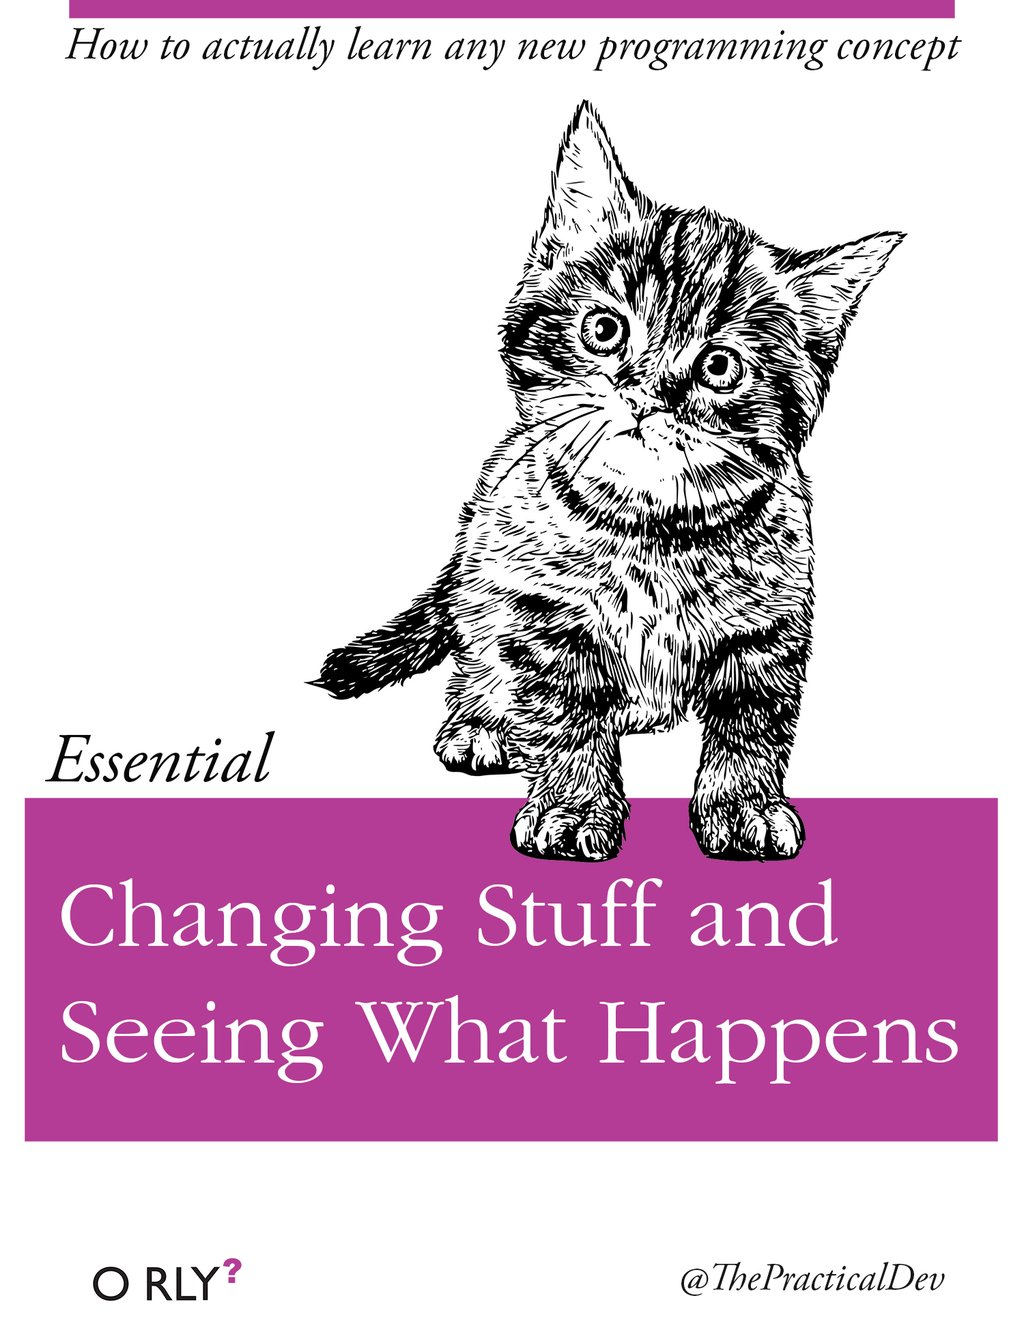
\includegraphics{img/practicalDev_changingstuff.jpg}
\caption{}
\end{figure}

See
\href{https://guides.github.com/features/mastering-markdown/}{Mastering
Markdown · GitHub Guides} and add some more personalized content to the
README of your own, like a bulleted list or blockquote. For on the fly
rendering, the \href{https://atom.io/}{atom} text editor is good.

\section{Intro to Markdown}\label{intro-to-markdown}

\subsection{from GitHub.com}\label{from-github.com}

Let's learn markdown by editing the \texttt{README.md} on github.com for
convenience. A README.md file can be added to every folder in a
repository, and they are automatically displayed when the repository is
opened on github.com

The \texttt{README.md} is in \textbf{markdown}, simple syntax for
conversion to HTML. \texttt{.md} is a kind of text file, so you only
need a text editor to read it. If you were editing this on your
computer, you could do this right in RStudio, which has a built-in text
editor. (You could also do it in another text editor program, but
RStudio is convenient). Copy-paste the following into your
\texttt{README.md}:

\begin{verbatim}
# my-project

This project is based on [Collaborative, Reproducible Science training ](https://ohi-science.org/data-science-training/).

## Introduction

Markdown syntax changes plain text to **bold** and *italics*:

1. **Git**
1. **Github**
1. *Markdown*
1. *Rmarkdown*

## Conclusion

![](https://octodex.github.com/images/labtocat.png)
\end{verbatim}

Notice the syntax for:

\begin{itemize}
\tightlist
\item
  \textbf{headers} get rendered at multiple levels: \texttt{\#},
  \texttt{\#\#}
\item
  \textbf{link}: \texttt{{[}{]}(http://...)}
\item
  \textbf{image}: \texttt{!{[}{]}(http://...)} --- note the \texttt{!}
\item
  \emph{italics}: \texttt{*word*}
\item
  \textbf{bold}: \texttt{**word**}
\item
  \textbf{numbered list} gets automatically sequenced: \texttt{1.},
  \texttt{1.}
\end{itemize}

\subsection{from RStudio}\label{from-rstudio}

Let's go back to RStudio. Pull so that you have the most recent version
of your README locally. Let's open it and have a look. Documentation is
a really important part of coding, so let's look at the README. If we
look at GitHub.com, you can see that the README is displayed nicely like
online. Let's add some more description about what our GitHub repository
is for.

Now click on the Preview button to see the markdown rendered as HTML.

Let's change the image to the plot we made yesterday.

\texttt{!{[}{]}(my\_plot.png)}

There are some good
\href{https://github.com/adam-p/markdown-here/wiki/Markdown-Here-Cheatsheet}{cheatsheets}
to get you started, and here is one built into RStudio:

\begin{figure}[htbp]
\centering
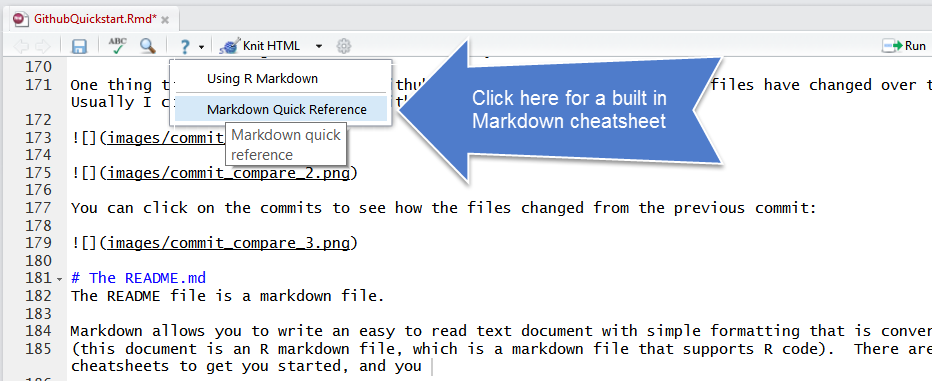
\includegraphics{img/md_cheatsheet.png}
\caption{}
\end{figure}

knit with the button; also \texttt{knitr}

\subsection{Your turn}\label{your-turn-12}

Update the README, push to GitHub

\section{RMarkdown from RStudio}\label{rmarkdown-from-rstudio}

Back in RStudio, let's create a new RMarkdown file, which allows us to
weave markdown text with chunks of R code to be evaluated and output
content like tables and plots.

File -\textgreater{} New File -\textgreater{} RMarkdown\ldots{}
-\textgreater{} Document of output format HTML, OK.

You can give it a Title of ``My Project''. After you click OK, most
importantly File -\textgreater{} Save as \texttt{index} (which will get
named with the filename extension \texttt{index.Rmd}).

Some initial text is already provided for you. Let's go ahead and ``Knit
HTML''.

Notice how the markdown is rendered similar to as before + \textbf{R
code chunks} are surrounded by 3 backticks and \texttt{\{r\ LABEL\}}.
These are evaluated and return the output text in the case of
\texttt{summary(cars)} and the output plot in the case of
\texttt{plot(pressure)}.

Notice how the code \texttt{plot(pressure)} is not shown in the HTML
output because of the R code chunk option \texttt{echo=FALSE}.

\textbf{Before we continue exploring Rmarkdown}, let's sync this the
.rmd and .html to github.com. Enter a message like ``added index'' and
click on ``Commit and Sync gh-pages''. This will update
\url{https://github.com/USER/my-project}, and now you can also see your
project website with a default \texttt{index.html} viewable at
\url{http://USER.github.io/my-project}

\subsection{Your turn}\label{your-turn-13}

\section{Resources}\label{resources-2}

Were you hoping for an RStudio Cheatsheet? Here it is:

\begin{itemize}
\tightlist
\item
  \href{http://www.rstudio.com/wp-content/uploads/2016/03/rmarkdown-cheatsheet-2.0.pdf}{rmarkdown-cheatsheet.pdf}
\item
  \url{http://rmarkdown.rstudio.com}
\item
  \href{http://kbroman.org/knitr_knutshell/}{knitr in a knutshell - Karl
  Broman}
\end{itemize}

save, commit, push

\section{More practice data wrangling, data
viz}\label{more-practice-data-wrangling-data-viz}

let's do it from our RMarkdown now. MORE DPLYR (GROUP BY?), AND TIDYR.
MAYBE MORE GGPLOT2?

\subsection{Your turn}\label{your-turn-14}

\section{Troubleshooting}\label{troubleshooting-4}

\chapter{Collaborate with GitHub}\label{collaborate}

\section{Objectives and Resources}\label{objectives-and-resources-1}

\textbf{Objectives}

\begin{itemize}
\tightlist
\item
  contribute to a repo that you don't own
\item
  give permission to a collaborator
\item
  open as a new RStudio project!
\item
  collaborate with a partner, explore github.com blame, history
\item
  practice more ggplot2 collab
\end{itemize}

\begin{enumerate}
\def\labelenumi{\arabic{enumi}.}
\tightlist
\item
  add their neighbor as a collaborator to their repo
\item
  practice more; make changes to their repo, and to their neighbor's.
\end{enumerate}

\textbf{Resources}

\section{pull request to your friend's
repo}\label{pull-request-to-your-friends-repo}

\section{create gh-pages repo and give someone
permission}\label{create-gh-pages-repo-and-give-someone-permission}

\begin{itemize}
\tightlist
\item
  Rmd analysis
\end{itemize}


\end{document}
